\documentclass[11pt,a4paper]{amsart}
\usepackage[a4paper,landscape,margin=20mm]{geometry}
\usepackage{amsmath,amssymb,amsthm,mathtools,stmaryrd,graphicx,xcolor}
\usepackage[no-math]{fontspec}
\setmainfont{lmroman10-regular.otf}[BoldFont=lmroman10-bold.otf,ItalicFont=lmroman10-italic.otf,BoldItalicFont=lmroman10-bolditalic.otf,SmallCapsFont=lmromancaps10-regular.otf]
\usepackage{hyperref}
\AtBeginDocument{\def\shorttitle{Probabilistic infinite trace equivalence}}
\title{A complete inference system for probabilistic infinite trace equivalence}
\author{Corina Cîrstea, Lawrence S. Moss, Victoria Noquez, Todd Schmid, Alexandra Silva, Ana Sokolova}
\date{doi:10.4230/LIPIcs.CSL.2025.30; CC BY 4.0}
\begin{document}
\maketitle
\noindent\textit{Editorial scope.} One infinite-trace inference-completeness main group. Complete official CC BY4 published HTML/PDF source used; prior soundness/support not additional counts. All original credits retained.\par\medskip
\noindent\textit{Allowed standard prerequisites (editorial).}\begin{itemize}
\item Convex algebras, probability measures and standard trace soundness. All original definitions and cited standard category/probability facts retained. Prior soundness is explicitly author-cited [21, Thm6.9]; new completeness and its final-coalgebra/proper-convex-functor arguments are collected in full, not replaced by a citation.
\end{itemize}\medskip
%
% SOURCE HTML #abstract
\hypertarget{html:abstract}{} \par\noindent\textbf{Abstract}\quad  We present the first sound and complete axiomatization of \emph{infinite} trace semantics for generative probabilistic transition systems. Our approach is categorical, and we build on recent results on proper functors over convex sets. At the core of our proof is a characterization of infinite traces as the final coalgebra of a functor over convex algebras. Somewhat surprisingly, our axiomatization of infinite trace semantics coincides with that of finite trace semantics, even though the techniques used in the completeness proof are significantly different.
\par\medskip
 
 \par\noindent\textbf{Funding:}\quad Corina Cîrstea: partly supported by the Leverhulme Trust Research Project Grant RPG-2020-232. 
 \par\noindent\textbf{Acknowledgements:}\quad We thank Wojtek Rozowski for insightful discussions on related topics and the anonymous reviewers for helpful suggestions that improved the material presented in the paper. We thank the National Science Foundation and the Simons Laufer Mathematical Sciences Institute for their support of our work. 
 \par\noindent\textbf{Funding:}\quad This material is based upon work supported by the National Science Foundation under Grant No. DMS-1928930, while the authors were in residence at the Mathematical Sciences Research Institute in Berkeley, California, during the Summer Research in Mathematics program of 2024. 
%
\par\noindent\textbf{Funding (original publisher PDF page1 and article metadata):} Lawrence S. Moss: Lawrence S. Moss was supported by grant \#586136 from the Simons Foundation. Alexandra Silva: ERC grant Autoprobe (no. 101002697). This work was done in part while the author was visiting the Simons Institute for the Theory of Computing.\par\medskip
% SOURCE HTML #S1
\hypertarget{html:S1}{} \section*{1 Introduction}
 %
% SOURCE HTML #S1.p1
\hypertarget{html:S1.p1}{} Probabilistic transition systems have been studied in the semantics and verification literature for decades. There are many variants, from the simplest Rabin model [\hyperlink{html:bib.bib16}{16}] to systems that encompass multiple layers of randomized and non-deterministic choice. A good overview of existing systems and an expressiveness hierarchy was provided in [\hyperlink{html:bib.bib26}{26}, \hyperlink{html:bib.bib3}{3}].
\par\medskip
  %
% SOURCE HTML #S1.p2
\hypertarget{html:S1.p2}{} One important class of probabilistic systems are so-called \emph{generative} probabilistic transition systems (GPTS). These are much like ordinary (nondeterministic) labelled transition systems, but each state is assigned a (sub-)probability distribution over outgoing transitions instead of a set of outgoing transitions. Every state in a GPTS \emph{generates} a probability distribution of traces. The traces generated can be \emph{finite} or \emph{infinite} depending whether the GPTS models \emph{explicit termination}.
\par\medskip
  %
% SOURCE HTML #S1.p3
\hypertarget{html:S1.p3}{} In this paper, we will consider GPTS \emph{without} explicit termination, also widely known in the literature as Labelled Markov Chains (LMCs), and therefore we are only interested in including infinite traces in the semantics. That is, each state of an LMC we consider generates a probability distribution on infinite traces (a.k.a. streams). The main goal of this paper is to provide an axiomatic characterization of when two states in these LMCs generate the same probability distribution on streams. We provide a syntax and an inference system to reason about distributions on streams generated by a state of an LMC, and prove that the axiomatization is both sound and complete.
\par\medskip
  %
% SOURCE HTML #S1.p4
\hypertarget{html:S1.p4}{} Axiomatizing trace distribution semantics is difficult in general, and this is made more challenging by the presence of infinite traces. One of the seminal works on axiomatizing probabilistic behaviours is due to Stark and Smolka [\hyperlink{html:bib.bib29}{29}], but they studied probabilistic bisimilarity (in the sense of [\hyperlink{html:bib.bib11}{11}]), which is a finer equivalence than trace distributions. A decade later [\hyperlink{html:bib.bib25}{25}], Silva and Sokolova showed that adding one extra axiom to Stark and Smolka’s axiomatization of probabilistic bisimilarity was enough to obtain a sound and complete axiomatization of \emph{finite} trace distribution equivalence. At the core of Silva and Sokolova’s completeness result was the observation that finite trace distribution equivalence coincides with bisimilarity after determinization in the category of \emph{convex algebras}, algebraic structures that model the closure of convex sets under convex combinations. Stark and Smolka’s result is the probabilistic analogue of an earlier paper of Milner [\hyperlink{html:bib.bib15}{15}], whereas Silva and Sokolova’s is the probabilistic analogue of an earlier paper of Rabinovich [\hyperlink{html:bib.bib17}{17}], where it is shown that a sound and complete axiomatization of trace semantics of labelled transition systems can be obtained from an axiomatization of bisimilarity. All these works, non-deterministic and probabilistic, restrict themselves to \emph{finite traces}.
\par\medskip
  %
% SOURCE HTML #S1.p5
\hypertarget{html:S1.p5}{} To achieve our goal, we use a categorical perspective on the semantics of LMCs. This is in the spirit of [\hyperlink{html:bib.bib25}{25}], but there are crucial technical hurdles to overcome: First, we need to find an endofunctor on a category that models LMCs as coalgebras and allows the derivation of the stream distribution semantics in a canonical way. More specifically, we need to give a coalgebraic characterization of the map that assigns to every state of an LMC the distribution on streams that the state generates. To this end, we carefully craft the endofunctor %
% SOURCE HTML #S1.p5.m1
\hypertarget{html:S1.p5.m1}{}\({G}\) on the category %
% SOURCE HTML #S1.p5.m2
\hypertarget{html:S1.p5.m2}{}\({\mathsf{CA}}\) of convex algebras and convex algebra homomorphisms in \hyperlink{html:S5}{Section 5}. Second, we show that our endofunctor satisfies a number of desirable properties that enable a sound and complete axiomatization, including the preservation of pullbacks and \emph{properness} [\hyperlink{html:bib.bib14}{14}]. Finally, we need to find a suitable syntax for specifying finite LMCs where stream semantics is of interest. Each of these steps pushes the boundaries of existing work on semantics and decidability of trace equivalence for automata, and they require new technical results that form the core contributions of our paper. We briefly describe our contributions below and give an outline of the paper.
\par\medskip
 %
% SOURCE HTML #S1.I1
\hypertarget{html:S1.I1}{}
\begin{list}{}{\leftmargin=2em}
 %
% SOURCE HTML #S1.I1.i1
\hypertarget{html:S1.I1.i1}{}
\item[]  %
% SOURCE HTML #S1.I1.i1.m1
\hypertarget{html:S1.I1.i1.m1}{}\({\blacksquare}\) %
% SOURCE HTML #S1.I1.i1.p1
\hypertarget{html:S1.I1.i1.p1}{} In \hyperlink{html:S2}{Section 2}, we recall basic definitions on labelled Markov chains and their semantics.
\par\medskip
  
 %
% SOURCE HTML #S1.I1.i2
\hypertarget{html:S1.I1.i2}{}
\item[]  %
% SOURCE HTML #S1.I1.i2.m1
\hypertarget{html:S1.I1.i2.m1}{}\({\blacksquare}\) %
% SOURCE HTML #S1.I1.i2.p1
\hypertarget{html:S1.I1.i2.p1}{} In \hyperlink{html:S3}{Section 3}, we recall the syntax of Stark and Smolka’s process algebra [\hyperlink{html:bib.bib29}{29}] and Silva and Sokolova’s axioms for finite trace equivalence [\hyperlink{html:bib.bib23}{23}], which will form the basis of our inference system and allow us to state our intended soundness and completeness results.
\par\medskip
  
 %
% SOURCE HTML #S1.I1.i3
\hypertarget{html:S1.I1.i3}{}
\item[]  %
% SOURCE HTML #S1.I1.i3.m1
\hypertarget{html:S1.I1.i3.m1}{}\({\blacksquare}\) %
% SOURCE HTML #S1.I1.i3.p1
\hypertarget{html:S1.I1.i3.p1}{} In \hyperlink{html:S4}{Section 4}, we explain our high-level strategy for proving completeness, which follows the \emph{coalgebraic completeness method} described in [\hyperlink{html:bib.bib22}{22}] that originates in [\hyperlink{html:bib.bib8}{8}, \hyperlink{html:bib.bib24}{24}, \hyperlink{html:bib.bib13}{13}].
\par\medskip
  
 %
% SOURCE HTML #S1.I1.i4
\hypertarget{html:S1.I1.i4}{}
\item[]  %
% SOURCE HTML #S1.I1.i4.m1
\hypertarget{html:S1.I1.i4.m1}{}\({\blacksquare}\) %
% SOURCE HTML #S1.I1.i4.p1
\hypertarget{html:S1.I1.i4.p1}{} In \hyperlink{html:S5}{Section 5}, we define the endofunctor %
% SOURCE HTML #S1.I1.i4.p1.m1
\hypertarget{html:S1.I1.i4.p1.m1}{}\({G}\), which forms the basis of all of our developments. The functor %
% SOURCE HTML #S1.I1.i4.p1.m2
\hypertarget{html:S1.I1.i4.p1.m2}{}\({G}\) is defined on the category %
% SOURCE HTML #S1.I1.i4.p1.m3
\hypertarget{html:S1.I1.i4.p1.m3}{}\({\mathsf{CA}}\) of convex algebras and convex algebra homomorphisms (see \hyperlink{html:S4.Thmtheorem1}{Definition 4.1}), and makes use of an important \emph{mass-splitting property} that resembles a side condition present in [\hyperlink{html:bib.bib6}{6}]. Crucially, we characterize stream distribution semantics as a final %
% SOURCE HTML #S1.I1.i4.p1.m4
\hypertarget{html:S1.I1.i4.p1.m4}{}\({G}\)-coalgebra semantics, via a \emph{determinization} construction that turns LMCs into %
% SOURCE HTML #S1.I1.i4.p1.m5
\hypertarget{html:S1.I1.i4.p1.m5}{}\({G}\)-coalgebras. This construction is interesting in its own right, given its simplicity compared to existing finality-based approaches to infinite trace semantics [\hyperlink{html:bib.bib9}{9}, \hyperlink{html:bib.bib5}{5}, \hyperlink{html:bib.bib6}{6}].
\par\medskip
  
 %
% SOURCE HTML #S1.I1.i5
\hypertarget{html:S1.I1.i5}{}
\item[]  %
% SOURCE HTML #S1.I1.i5.m1
\hypertarget{html:S1.I1.i5.m1}{}\({\blacksquare}\) %
% SOURCE HTML #S1.I1.i5.p1
\hypertarget{html:S1.I1.i5.p1}{} In \hyperlink{html:S6}{Section 6}, we define a %
% SOURCE HTML #S1.I1.i5.p1.m1
\hypertarget{html:S1.I1.i5.p1.m1}{}\({G}\)-coalgebra structure on the set of process terms modulo axioms, which endows the terms with an operational semantics. We show that this term coalgebra is universal among the free and finitely generated %
% SOURCE HTML #S1.I1.i5.p1.m2
\hypertarget{html:S1.I1.i5.p1.m2}{}\({G}\)-coalgebras by providing unique solutions to finite systems of equations arising from a coalgebra structure.
\par\medskip
  
 %
% SOURCE HTML #S1.I1.i6
\hypertarget{html:S1.I1.i6}{}
\item[]  %
% SOURCE HTML #S1.I1.i6.m1
\hypertarget{html:S1.I1.i6.m1}{}\({\blacksquare}\) %
% SOURCE HTML #S1.I1.i6.p1
\hypertarget{html:S1.I1.i6.p1}{} In \hyperlink{html:S7}{Section 7}, we conclude our proof of completeness by establishing that %
% SOURCE HTML #S1.I1.i6.p1.m1
\hypertarget{html:S1.I1.i6.p1.m1}{}\({G}\) satisfies a property called \emph{properness}, introduced by Milius in [\hyperlink{html:bib.bib14}{14}]. The proof that %
% SOURCE HTML #S1.I1.i6.p1.m2
\hypertarget{html:S1.I1.i6.p1.m2}{}\({G}\) is proper uses a topological characterization of congruences of finitely generated convex algebras due to Sokolova and Woraceck [\hyperlink{html:bib.bib27}{27}].
\par\medskip
  
 %
% SOURCE HTML #S1.I1.i7
\hypertarget{html:S1.I1.i7}{}
\item[]  %
% SOURCE HTML #S1.I1.i7.m1
\hypertarget{html:S1.I1.i7.m1}{}\({\blacksquare}\) %
% SOURCE HTML #S1.I1.i7.p1
\hypertarget{html:S1.I1.i7.p1}{} We conclude with a discussion of related and future work, and the implications of the completeness theorem in \hyperlink{html:S8}{Section 8}.
\par\medskip
  
 
\end{list}
  %
% SOURCE HTML #S1.p6
\hypertarget{html:S1.p6}{} Our completeness result is remarkable for two reasons: First and foremost, our axiomatization is precisely the same as Silva and Sokolova’s for finite trace semantics. In other words, both the (finite) trace distribution semantics and the stream distribution semantics give rise to the same valid equations between term expressions. Second, the completeness result uses a novel proof of properness [\hyperlink{html:bib.bib14}{14}, \hyperlink{html:bib.bib28}{28}] that appears to hinge on the topology of bisimulations between coalgebras over convex algebras. The latter is a significant point of departure from the properness proof method of Sokolova and Woracek [\hyperlink{html:bib.bib28}{28}].
\par\medskip
  
%
% SOURCE HTML #S2
\hypertarget{html:S2}{} \section*{2 Labelled Markov Chains and Stream Semantics}
 %
% SOURCE HTML #S2.p1
\hypertarget{html:S2.p1}{} In this section, we briefly recall basic definitions of labelled Markov chains, stream semantics, and the framework of universal coalgebra.
\par\medskip
  %
% SOURCE HTML #S2.SS0.SSS0.P0.SPx1
\hypertarget{html:S2.SS0.SSS0.P0.SPx1}{} \par\noindent\textbf{Labelled Markov chains.}\quad  %
% SOURCE HTML #S2.SS0.SSS0.P0.SPx1.p1
\hypertarget{html:S2.SS0.SSS0.P0.SPx1.p1}{} Given a set %
% SOURCE HTML #S2.SS0.SSS0.P0.SPx1.p1.m1
\hypertarget{html:S2.SS0.SSS0.P0.SPx1.p1.m1}{}\({X}\), define %
% SOURCE HTML #S2.SS0.SSS0.P0.SPx1.p1.m2
\hypertarget{html:S2.SS0.SSS0.P0.SPx1.p1.m2}{}\({{\mathcal{D}}(X)}\) to be the set of finitely supported probability distributions on %
% SOURCE HTML #S2.SS0.SSS0.P0.SPx1.p1.m3
\hypertarget{html:S2.SS0.SSS0.P0.SPx1.p1.m3}{}\({X}\). That is, %
% SOURCE HTML #S2.SS0.SSS0.P0.SPx1.p1.m4
\hypertarget{html:S2.SS0.SSS0.P0.SPx1.p1.m4}{}\({\theta\in{\mathcal{D}}(X)}\) if and only if %
% SOURCE HTML #S2.SS0.SSS0.P0.SPx1.p1.m5
\hypertarget{html:S2.SS0.SSS0.P0.SPx1.p1.m5}{}\({\theta\colon X\to[0,1]}\), %
% SOURCE HTML #S2.SS0.SSS0.P0.SPx1.p1.m6
\hypertarget{html:S2.SS0.SSS0.P0.SPx1.p1.m6}{}\({\theta(x)>0}\) for finitely many %
% SOURCE HTML #S2.SS0.SSS0.P0.SPx1.p1.m7
\hypertarget{html:S2.SS0.SSS0.P0.SPx1.p1.m7}{}\({x\in X}\), and %
% SOURCE HTML #S2.SS0.SSS0.P0.SPx1.p1.m8
\hypertarget{html:S2.SS0.SSS0.P0.SPx1.p1.m8}{}\({\theta(X)=\sum_{x\in X}\theta(x)=1}\). Since the support is finite, each %
% SOURCE HTML #S2.SS0.SSS0.P0.SPx1.p1.m9
\hypertarget{html:S2.SS0.SSS0.P0.SPx1.p1.m9}{}\({\theta\in{\mathcal{D}}(X)}\) can be written in the form %
% SOURCE HTML #S2.SS0.SSS0.P0.SPx1.p1.m10
\hypertarget{html:S2.SS0.SSS0.P0.SPx1.p1.m10}{}\({\sum_{i=1}^{n}r_{i}\cdot x_{i}}\) such that %
% SOURCE HTML #S2.SS0.SSS0.P0.SPx1.p1.m11
\hypertarget{html:S2.SS0.SSS0.P0.SPx1.p1.m11}{}\({r_{i}\in(0,1]}\) and %
% SOURCE HTML #S2.SS0.SSS0.P0.SPx1.p1.m12
\hypertarget{html:S2.SS0.SSS0.P0.SPx1.p1.m12}{}\({x_{i}\in X}\) for each %
% SOURCE HTML #S2.SS0.SSS0.P0.SPx1.p1.m13
\hypertarget{html:S2.SS0.SSS0.P0.SPx1.p1.m13}{}\({i\leq n}\). We write %
% SOURCE HTML #S2.SS0.SSS0.P0.SPx1.p1.m14
\hypertarget{html:S2.SS0.SSS0.P0.SPx1.p1.m14}{}\({1\cdot x}\) for the \emph{Dirac delta} at %
% SOURCE HTML #S2.SS0.SSS0.P0.SPx1.p1.m15
\hypertarget{html:S2.SS0.SSS0.P0.SPx1.p1.m15}{}\({x\in X}\).
\par\medskip
  %
% SOURCE HTML #S2.SS0.SSS0.P0.SPx1.p2
\hypertarget{html:S2.SS0.SSS0.P0.SPx1.p2}{} For a fixed finite set %
% SOURCE HTML #S2.SS0.SSS0.P0.SPx1.p2.m1
\hypertarget{html:S2.SS0.SSS0.P0.SPx1.p2.m1}{}\({A}\) of formal symbols called \emph{actions}, a \emph{labelled Markov chain} (or \emph{LMC}) is a pair %
% SOURCE HTML #S2.SS0.SSS0.P0.SPx1.p2.m2
\hypertarget{html:S2.SS0.SSS0.P0.SPx1.p2.m2}{}\({(X,\beta)}\) consisting of a set %
% SOURCE HTML #S2.SS0.SSS0.P0.SPx1.p2.m3
\hypertarget{html:S2.SS0.SSS0.P0.SPx1.p2.m3}{}\({X}\) of \emph{states} and a \emph{transition function} %
% SOURCE HTML #S2.SS0.SSS0.P0.SPx1.p2.m4
\hypertarget{html:S2.SS0.SSS0.P0.SPx1.p2.m4}{}\({\beta\colon X\to{\mathcal{D}}(A\times X)}\). An LMC is said to be \emph{finite} if it has finitely many states.
\par\medskip
  %
% SOURCE HTML #S2.SS0.SSS0.P0.SPx1.p3
\hypertarget{html:S2.SS0.SSS0.P0.SPx1.p3}{} One graphical depiction of a finite LMC is the directed graph with a node for each state and a decorated edge %
% SOURCE HTML #S2.SS0.SSS0.P0.SPx1.p3.m1
\hypertarget{html:S2.SS0.SSS0.P0.SPx1.p3.m1}{}\({x\mathrel{\raisebox{-2.0pt}{$\xrightarrow{a\mid r}$}}_{\beta}y}\) between nodes %
% SOURCE HTML #S2.SS0.SSS0.P0.SPx1.p3.m2
\hypertarget{html:S2.SS0.SSS0.P0.SPx1.p3.m2}{}\({x}\) and %
% SOURCE HTML #S2.SS0.SSS0.P0.SPx1.p3.m3
\hypertarget{html:S2.SS0.SSS0.P0.SPx1.p3.m3}{}\({y}\) whenever %
% SOURCE HTML #S2.SS0.SSS0.P0.SPx1.p3.m4
\hypertarget{html:S2.SS0.SSS0.P0.SPx1.p3.m4}{}\({\beta(x)(a,y)=r}\) with %
% SOURCE HTML #S2.SS0.SSS0.P0.SPx1.p3.m5
\hypertarget{html:S2.SS0.SSS0.P0.SPx1.p3.m5}{}\({r>0}\). We typically drop the %
% SOURCE HTML #S2.SS0.SSS0.P0.SPx1.p3.m6
\hypertarget{html:S2.SS0.SSS0.P0.SPx1.p3.m6}{}\({\beta}\) notation whenever the transition function is clear from context.
\par\medskip
  %
% SOURCE HTML #S2.Thmtheorem1
\hypertarget{html:S2.Thmtheorem1}{} \par\noindent\textbf{\textbf{Example 2.1}\textbf{.}}\quad  %
% SOURCE HTML #S2.Thmtheorem1.p1
\hypertarget{html:S2.Thmtheorem1.p1}{} \emph{The LMC %
% SOURCE HTML #S2.Thmtheorem1.p1.m1
\hypertarget{html:S2.Thmtheorem1.p1.m1}{}\({(X,\beta\colon X\to{\mathcal{D}}(A\times X))}\) with %
% SOURCE HTML #S2.Thmtheorem1.p1.m2
\hypertarget{html:S2.Thmtheorem1.p1.m2}{}\({A=\{a,b\}}\), %
% SOURCE HTML #S2.Thmtheorem1.p1.m3
\hypertarget{html:S2.Thmtheorem1.p1.m3}{}\({X=\{x,y\}}\), and %
% SOURCE HTML #S2.Thmtheorem1.p1.m4
\hypertarget{html:S2.Thmtheorem1.p1.m4}{}\({\beta(x)(a,y)=\beta(x)(b,x)=\beta(y)(b,x)=\beta(y)(a,y)=0.5}\) is depicted in (\hyperlink{html:S2.E1}{2.1}).}
\par\medskip
 %
% SOURCE HTML #S2.E1
\hypertarget{html:S2.E1}{}   %
% SOURCE HTML #S2.E1.m1.g1
\hypertarget{html:S2.E1.m1.g1}{}\begin{center}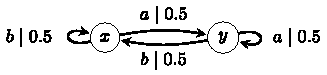
\includegraphics[width=157pt]{S2.E1.m1.g1.pdf}\end{center}
  (2.1)      %
% SOURCE HTML #S2.SS0.SSS0.P0.SPx2
\hypertarget{html:S2.SS0.SSS0.P0.SPx2}{} \par\noindent\textbf{Stream semantics.}\quad  %
% SOURCE HTML #S2.SS0.SSS0.P0.SPx2.p1
\hypertarget{html:S2.SS0.SSS0.P0.SPx2.p1}{} A \emph{word} over a finite alphabet %
% SOURCE HTML #S2.SS0.SSS0.P0.SPx2.p1.m1
\hypertarget{html:S2.SS0.SSS0.P0.SPx2.p1.m1}{}\({A}\) is a finite sequence %
% SOURCE HTML #S2.SS0.SSS0.P0.SPx2.p1.m2
\hypertarget{html:S2.SS0.SSS0.P0.SPx2.p1.m2}{}\({a_{1}\cdots a_{n}}\) (written as a juxtaposition) of elements of %
% SOURCE HTML #S2.SS0.SSS0.P0.SPx2.p1.m3
\hypertarget{html:S2.SS0.SSS0.P0.SPx2.p1.m3}{}\({A}\). We write %
% SOURCE HTML #S2.SS0.SSS0.P0.SPx2.p1.m4
\hypertarget{html:S2.SS0.SSS0.P0.SPx2.p1.m4}{}\({\varepsilon}\) for the \emph{empty} word. A \emph{stream} is an infinite sequence %
% SOURCE HTML #S2.SS0.SSS0.P0.SPx2.p1.m5
\hypertarget{html:S2.SS0.SSS0.P0.SPx2.p1.m5}{}\({(a_{1},a_{2},\dots)}\) of elements from %
% SOURCE HTML #S2.SS0.SSS0.P0.SPx2.p1.m6
\hypertarget{html:S2.SS0.SSS0.P0.SPx2.p1.m6}{}\({A}\). We write %
% SOURCE HTML #S2.SS0.SSS0.P0.SPx2.p1.m7
\hypertarget{html:S2.SS0.SSS0.P0.SPx2.p1.m7}{}\({A^{*}}\) for the set of words and %
% SOURCE HTML #S2.SS0.SSS0.P0.SPx2.p1.m8
\hypertarget{html:S2.SS0.SSS0.P0.SPx2.p1.m8}{}\({A^{\omega}}\) for the set of streams. The set %
% SOURCE HTML #S2.SS0.SSS0.P0.SPx2.p1.m9
\hypertarget{html:S2.SS0.SSS0.P0.SPx2.p1.m9}{}\({A^{\omega}}\) carries a topology, with basis given by the \emph{cylinder sets},
\par\medskip
 %
% SOURCE HTML #S2.Ex1
\hypertarget{html:S2.Ex1}{}   %
% SOURCE HTML #S2.Ex1.m1
\hypertarget{html:S2.Ex1.m1}{}\[B_{w}=\{(a_{1},\dots,a_{n},\ldots)\mid a_{1}\cdots a_{n}=w\}\]    where %
% SOURCE HTML #S2.SS0.SSS0.P0.SPx2.p1.m10
\hypertarget{html:S2.SS0.SSS0.P0.SPx2.p1.m10}{}\({w\in A^{*}}\) is a word. In the notation above, %
% SOURCE HTML #S2.SS0.SSS0.P0.SPx2.p1.m11
\hypertarget{html:S2.SS0.SSS0.P0.SPx2.p1.m11}{}\({B_{\varepsilon}=A^{\omega}}\), as every stream begins with %
% SOURCE HTML #S2.SS0.SSS0.P0.SPx2.p1.m12
\hypertarget{html:S2.SS0.SSS0.P0.SPx2.p1.m12}{}\({\varepsilon}\).
\par\medskip
  %
% SOURCE HTML #S2.SS0.SSS0.P0.SPx2.p2
\hypertarget{html:S2.SS0.SSS0.P0.SPx2.p2}{} Recall that a \emph{Borel set} is an element of the %
% SOURCE HTML #S2.SS0.SSS0.P0.SPx2.p2.m1
\hypertarget{html:S2.SS0.SSS0.P0.SPx2.p2.m1}{}\({\sigma}\)-algebra generated by the open sets of a topological space, a \emph{Borel measure} is a measure defined on the Borel sets, and a \emph{Borel probability distribution} is a Borel measure with total probability %
% SOURCE HTML #S2.SS0.SSS0.P0.SPx2.p2.m2
\hypertarget{html:S2.SS0.SSS0.P0.SPx2.p2.m2}{}\({1}\) [\hyperlink{html:bib.bib19}{19}].
\par\medskip
  %
% SOURCE HTML #S2.Thmtheorem2
\hypertarget{html:S2.Thmtheorem2}{} \par\noindent\textbf{\textbf{Definition 2.2}\textbf{.}}\quad  %
% SOURCE HTML #S2.Thmtheorem2.p1
\hypertarget{html:S2.Thmtheorem2.p1}{} \emph{A \emph{stream distribution} is a Borel probability distribution on the space %
% SOURCE HTML #S2.Thmtheorem2.p1.m1
\hypertarget{html:S2.Thmtheorem2.p1.m1}{}\({A^{\omega}}\). The set of all stream distributions on %
% SOURCE HTML #S2.Thmtheorem2.p1.m2
\hypertarget{html:S2.Thmtheorem2.p1.m2}{}\({A^{\omega}}\) is written %
% SOURCE HTML #S2.Thmtheorem2.p1.m3
\hypertarget{html:S2.Thmtheorem2.p1.m3}{}\({\text{\sf Prob}(A^{\omega})}\).}
\par\medskip
   %
% SOURCE HTML #S2.SS0.SSS0.P0.SPx2.p3
\hypertarget{html:S2.SS0.SSS0.P0.SPx2.p3}{} Each state of an LMC corresponds to a unique stream distribution that records the probability of that state eventually emitting streams in a given Borel set. The following proposition is a special case of [\hyperlink{html:bib.bib9}{9}, Proposition 3.12].
\par\medskip
  %
% SOURCE HTML #S2.Thmtheorem3
\hypertarget{html:S2.Thmtheorem3}{} \par\noindent\textbf{\textbf{Proposition 2.3}\textbf{.}}\quad  %
% SOURCE HTML #S2.Thmtheorem3.p1
\hypertarget{html:S2.Thmtheorem3.p1}{} \emph{Let %
% SOURCE HTML #S2.Thmtheorem3.p1.m1
\hypertarget{html:S2.Thmtheorem3.p1.m1}{}\({(X,\beta)}\) be an LMC. There is a unique map %
% SOURCE HTML #S2.Thmtheorem3.p1.m2
\hypertarget{html:S2.Thmtheorem3.p1.m2}{}\({\left\llbracket{-}\right\rrbracket_{\beta}\colon X\to\text{\sf Prob}(A^{\omega})}\) such that for any %
% SOURCE HTML #S2.Thmtheorem3.p1.m3
\hypertarget{html:S2.Thmtheorem3.p1.m3}{}\({x\in X}\) and any %
% SOURCE HTML #S2.Thmtheorem3.p1.m4
\hypertarget{html:S2.Thmtheorem3.p1.m4}{}\({w\in A^{*}}\) and %
% SOURCE HTML #S2.Thmtheorem3.p1.m5
\hypertarget{html:S2.Thmtheorem3.p1.m5}{}\({a\in A}\),}
\par\medskip
 %
% SOURCE HTML #S2.Ex2
\hypertarget{html:S2.Ex2}{}   %
% SOURCE HTML #S2.Ex2.m1
\hypertarget{html:S2.Ex2.m1}{}\[\left\llbracket{x}\right\rrbracket_{\beta}(B_{aw})=\sum_{y\in X}\beta(x)(a,y)\left\llbracket{y}\right\rrbracket_{\beta}(B_{w})\]      %
% SOURCE HTML #S2.SS0.SSS0.P0.SPx2.p4
\hypertarget{html:S2.SS0.SSS0.P0.SPx2.p4}{} The map %
% SOURCE HTML #S2.SS0.SSS0.P0.SPx2.p4.m1
\hypertarget{html:S2.SS0.SSS0.P0.SPx2.p4.m1}{}\({\left\llbracket{-}\right\rrbracket_{\beta}}\) above is the \emph{stream semantics} of %
% SOURCE HTML #S2.SS0.SSS0.P0.SPx2.p4.m2
\hypertarget{html:S2.SS0.SSS0.P0.SPx2.p4.m2}{}\({(X,\beta)}\). Given states %
% SOURCE HTML #S2.SS0.SSS0.P0.SPx2.p4.m3
\hypertarget{html:S2.SS0.SSS0.P0.SPx2.p4.m3}{}\({x,y\in X}\), we say %
% SOURCE HTML #S2.SS0.SSS0.P0.SPx2.p4.m4
\hypertarget{html:S2.SS0.SSS0.P0.SPx2.p4.m4}{}\({x}\) and %
% SOURCE HTML #S2.SS0.SSS0.P0.SPx2.p4.m5
\hypertarget{html:S2.SS0.SSS0.P0.SPx2.p4.m5}{}\({y}\) are \emph{stream equivalent} if %
% SOURCE HTML #S2.SS0.SSS0.P0.SPx2.p4.m6
\hypertarget{html:S2.SS0.SSS0.P0.SPx2.p4.m6}{}\({\left\llbracket{x}\right\rrbracket_{\beta}=\left\llbracket{y}\right\rrbracket_{\beta}}\).
\par\medskip
   %
% SOURCE HTML #S2.SS0.SSS0.P0.SPx3
\hypertarget{html:S2.SS0.SSS0.P0.SPx3}{} \par\noindent\textbf{LMCs as coalgebras.}\quad  %
% SOURCE HTML #S2.SS0.SSS0.P0.SPx3.p1
\hypertarget{html:S2.SS0.SSS0.P0.SPx3.p1}{} Universal coalgebra is by now a standard framework for studying state-based systems like LMCs [\hyperlink{html:bib.bib20}{20}]. The theory is sufficiently general for capturing systems where the states come with additional structure. Systems with structured state spaces are central to the main result of this paper, so we state the definitions below for more general categories than the category %
% SOURCE HTML #S2.SS0.SSS0.P0.SPx3.p1.m1
\hypertarget{html:S2.SS0.SSS0.P0.SPx3.p1.m1}{}\({\mathsf{Set}}\) of sets and functions.
\par\medskip
  %
% SOURCE HTML #S2.Thmtheorem4
\hypertarget{html:S2.Thmtheorem4}{} \par\noindent\textbf{\textbf{Definition 2.4}\textbf{.}}\quad  %
% SOURCE HTML #S2.Thmtheorem4.p1
\hypertarget{html:S2.Thmtheorem4.p1}{} \emph{Given an endofunctor on a category %
% SOURCE HTML #S2.Thmtheorem4.p1.m1
\hypertarget{html:S2.Thmtheorem4.p1.m1}{}\({F\colon\mathsf{C}\to\mathsf{C}}\), an \emph{%
% SOURCE HTML #S2.Thmtheorem4.p1.m2
\hypertarget{html:S2.Thmtheorem4.p1.m2}{}\({F}\)-coalgebra} is a pair %
% SOURCE HTML #S2.Thmtheorem4.p1.m3
\hypertarget{html:S2.Thmtheorem4.p1.m3}{}\({(X,c)}\) consisting of an object %
% SOURCE HTML #S2.Thmtheorem4.p1.m4
\hypertarget{html:S2.Thmtheorem4.p1.m4}{}\({X}\) of %
% SOURCE HTML #S2.Thmtheorem4.p1.m5
\hypertarget{html:S2.Thmtheorem4.p1.m5}{}\({\mathsf{C}}\) and an arrow %
% SOURCE HTML #S2.Thmtheorem4.p1.m6
\hypertarget{html:S2.Thmtheorem4.p1.m6}{}\({c\colon X\to F(X)}\). A \emph{coalgebra homomorphism} %
% SOURCE HTML #S2.Thmtheorem4.p1.m7
\hypertarget{html:S2.Thmtheorem4.p1.m7}{}\({h\colon(X,c^{X})\to(Y,c^{Y})}\) is an arrow %
% SOURCE HTML #S2.Thmtheorem4.p1.m8
\hypertarget{html:S2.Thmtheorem4.p1.m8}{}\({h\colon X\to Y}\) such that %
% SOURCE HTML #S2.Thmtheorem4.p1.m9
\hypertarget{html:S2.Thmtheorem4.p1.m9}{}\({c^{Y}\circ h=F(h)\circ c^{X}}\). We write %
% SOURCE HTML #S2.Thmtheorem4.p1.m10
\hypertarget{html:S2.Thmtheorem4.p1.m10}{}\({\mbox{\sf Coalg}_{\mathsf{C}}(F)}\) for the category of %
% SOURCE HTML #S2.Thmtheorem4.p1.m11
\hypertarget{html:S2.Thmtheorem4.p1.m11}{}\({F}\)-coalgebras and their homomorphisms.}
\par\medskip
   %
% SOURCE HTML #S2.SS0.SSS0.P0.SPx3.p2
\hypertarget{html:S2.SS0.SSS0.P0.SPx3.p2}{} The set-mapping %
% SOURCE HTML #S2.SS0.SSS0.P0.SPx3.p2.m1
\hypertarget{html:S2.SS0.SSS0.P0.SPx3.p2.m1}{}\({X\mapsto{\mathcal{D}}(X)}\) is a functor, with action on functions given by
\par\medskip
 %
% SOURCE HTML #S2.Ex3
\hypertarget{html:S2.Ex3}{}   %
% SOURCE HTML #S2.Ex3.m1
\hypertarget{html:S2.Ex3.m1}{}\[{\mathcal{D}}(f)(\theta)=\sum_{i=1}^{n}r_{i}\cdot f(x_{i})\]    where %
% SOURCE HTML #S2.SS0.SSS0.P0.SPx3.p2.m2
\hypertarget{html:S2.SS0.SSS0.P0.SPx3.p2.m2}{}\({f\colon X\to Y}\) and %
% SOURCE HTML #S2.SS0.SSS0.P0.SPx3.p2.m3
\hypertarget{html:S2.SS0.SSS0.P0.SPx3.p2.m3}{}\({\theta=\sum_{i=1}^{n}r_{i}\cdot x_{i}}\). The set-mapping %
% SOURCE HTML #S2.SS0.SSS0.P0.SPx3.p2.m4
\hypertarget{html:S2.SS0.SSS0.P0.SPx3.p2.m4}{}\({X\mapsto A\times X}\) is also a functor, with the action on functions being %
% SOURCE HTML #S2.SS0.SSS0.P0.SPx3.p2.m5
\hypertarget{html:S2.SS0.SSS0.P0.SPx3.p2.m5}{}\({f\mapsto\mathrm{id}_{A}\times f}\). By composition, %
% SOURCE HTML #S2.SS0.SSS0.P0.SPx3.p2.m6
\hypertarget{html:S2.SS0.SSS0.P0.SPx3.p2.m6}{}\({{\mathcal{D}}(A\times-)}\) is an endofunctor on %
% SOURCE HTML #S2.SS0.SSS0.P0.SPx3.p2.m7
\hypertarget{html:S2.SS0.SSS0.P0.SPx3.p2.m7}{}\({\mathsf{Set}}\). The point is that LMCs are precisely %
% SOURCE HTML #S2.SS0.SSS0.P0.SPx3.p2.m8
\hypertarget{html:S2.SS0.SSS0.P0.SPx3.p2.m8}{}\({{\mathcal{D}}(A\times-)}\)-coalgebras. Unravelling the definitions, a coalgebra homomorphism between LMCs %
% SOURCE HTML #S2.SS0.SSS0.P0.SPx3.p2.m9
\hypertarget{html:S2.SS0.SSS0.P0.SPx3.p2.m9}{}\({h\colon(X,\beta)\to(Y,\vartheta)}\) is a function %
% SOURCE HTML #S2.SS0.SSS0.P0.SPx3.p2.m10
\hypertarget{html:S2.SS0.SSS0.P0.SPx3.p2.m10}{}\({h\colon X\to Y}\) such that for any %
% SOURCE HTML #S2.SS0.SSS0.P0.SPx3.p2.m11
\hypertarget{html:S2.SS0.SSS0.P0.SPx3.p2.m11}{}\({x\in X}\), if %
% SOURCE HTML #S2.SS0.SSS0.P0.SPx3.p2.m12
\hypertarget{html:S2.SS0.SSS0.P0.SPx3.p2.m12}{}\({\beta(x)=\sum_{i=1}^{n}r_{i}\cdot(a_{i},x_{i})}\), then
\par\medskip
 %
% SOURCE HTML #S2.Ex4
\hypertarget{html:S2.Ex4}{}   %
% SOURCE HTML #S2.Ex4.m1
\hypertarget{html:S2.Ex4.m1}{}\[\vartheta(h(x))=\sum_{i=1}^{n}r_{i}\cdot(a_{i},h(x_{i}))\]    Coalgebra homomorphisms are precisely the maps that preserve the branching-time behaviour of probabilistic systems.
\par\medskip
  %
% SOURCE HTML #S2.SS0.SSS0.P0.SPx3.p3
\hypertarget{html:S2.SS0.SSS0.P0.SPx3.p3}{} A category %
% SOURCE HTML #S2.SS0.SSS0.P0.SPx3.p3.m1
\hypertarget{html:S2.SS0.SSS0.P0.SPx3.p3.m1}{}\({\mathsf{C}}\) is \emph{concrete} if there is a faithful functor %
% SOURCE HTML #S2.SS0.SSS0.P0.SPx3.p3.m2
\hypertarget{html:S2.SS0.SSS0.P0.SPx3.p3.m2}{}\({U\colon\mathsf{C}\to\mathsf{Set}}\). An object %
% SOURCE HTML #S2.SS0.SSS0.P0.SPx3.p3.m3
\hypertarget{html:S2.SS0.SSS0.P0.SPx3.p3.m3}{}\({X}\) in a concrete category %
% SOURCE HTML #S2.SS0.SSS0.P0.SPx3.p3.m4
\hypertarget{html:S2.SS0.SSS0.P0.SPx3.p3.m4}{}\({\mathsf{C}}\) is essentially a set %
% SOURCE HTML #S2.SS0.SSS0.P0.SPx3.p3.m5
\hypertarget{html:S2.SS0.SSS0.P0.SPx3.p3.m5}{}\({U(X)}\) with additional structure, and arrows %
% SOURCE HTML #S2.SS0.SSS0.P0.SPx3.p3.m6
\hypertarget{html:S2.SS0.SSS0.P0.SPx3.p3.m6}{}\({X\to Y}\) are functions that preserve that structure. We write %
% SOURCE HTML #S2.SS0.SSS0.P0.SPx3.p3.m7
\hypertarget{html:S2.SS0.SSS0.P0.SPx3.p3.m7}{}\({x\in X}\) for %
% SOURCE HTML #S2.SS0.SSS0.P0.SPx3.p3.m8
\hypertarget{html:S2.SS0.SSS0.P0.SPx3.p3.m8}{}\({x\in U(X)}\). The category %
% SOURCE HTML #S2.SS0.SSS0.P0.SPx3.p3.m9
\hypertarget{html:S2.SS0.SSS0.P0.SPx3.p3.m9}{}\({\mathsf{Set}}\) is of course concrete, as witnessed by the identity functor.
\par\medskip
  %
% SOURCE HTML #S2.Thmtheorem5
\hypertarget{html:S2.Thmtheorem5}{} \par\noindent\textbf{\textbf{Definition 2.5}\textbf{.}}\quad  %
% SOURCE HTML #S2.Thmtheorem5.p1
\hypertarget{html:S2.Thmtheorem5.p1}{} \emph{Let %
% SOURCE HTML #S2.Thmtheorem5.p1.m1
\hypertarget{html:S2.Thmtheorem5.p1.m1}{}\({(X,c^{X})}\) and %
% SOURCE HTML #S2.Thmtheorem5.p1.m2
\hypertarget{html:S2.Thmtheorem5.p1.m2}{}\({(Y,c^{Y})}\) be %
% SOURCE HTML #S2.Thmtheorem5.p1.m3
\hypertarget{html:S2.Thmtheorem5.p1.m3}{}\({F}\)-coalgebras where %
% SOURCE HTML #S2.Thmtheorem5.p1.m4
\hypertarget{html:S2.Thmtheorem5.p1.m4}{}\({F\colon\mathsf{C}\to\mathsf{C}}\) and %
% SOURCE HTML #S2.Thmtheorem5.p1.m5
\hypertarget{html:S2.Thmtheorem5.p1.m5}{}\({\mathsf{C}}\) is concrete, %
% SOURCE HTML #S2.Thmtheorem5.p1.m6
\hypertarget{html:S2.Thmtheorem5.p1.m6}{}\({x\in X}\) and %
% SOURCE HTML #S2.Thmtheorem5.p1.m7
\hypertarget{html:S2.Thmtheorem5.p1.m7}{}\({y\in Y}\). We say %
% SOURCE HTML #S2.Thmtheorem5.p1.m8
\hypertarget{html:S2.Thmtheorem5.p1.m8}{}\({x}\) and %
% SOURCE HTML #S2.Thmtheorem5.p1.m9
\hypertarget{html:S2.Thmtheorem5.p1.m9}{}\({y}\) are \emph{behaviourally equivalent} and write %
% SOURCE HTML #S2.Thmtheorem5.p1.m10
\hypertarget{html:S2.Thmtheorem5.p1.m10}{}\({x\sim y}\) if there is a cospan %
% SOURCE HTML #S2.Thmtheorem5.p1.m11
\hypertarget{html:S2.Thmtheorem5.p1.m11}{}\({(X,c^{X})\stackrel{{\scriptstyle h}}{{\longrightarrow}}(Z,c^{Z})\stackrel{{\scriptstyle k}}{{\longleftarrow}}(Y,c^{Y})}\) in %
% SOURCE HTML #S2.Thmtheorem5.p1.m12
\hypertarget{html:S2.Thmtheorem5.p1.m12}{}\({\mbox{\sf Coalg}_{\mathsf{C}}(F)}\) such that %
% SOURCE HTML #S2.Thmtheorem5.p1.m13
\hypertarget{html:S2.Thmtheorem5.p1.m13}{}\({h(x)=k(y)}\).}
\par\medskip
   %
% SOURCE HTML #S2.SS0.SSS0.P0.SPx3.p4
\hypertarget{html:S2.SS0.SSS0.P0.SPx3.p4}{} For LMCs, behavioural equivalence (which coincides with probabilistic bisimilarity) implies stream equivalence [\hyperlink{html:bib.bib21}{21}, Theorem 6.7].
\par\medskip
  %
% SOURCE HTML #S2.Thmtheorem6
\hypertarget{html:S2.Thmtheorem6}{} \par\noindent\textbf{\textbf{Proposition 2.6}\textbf{.}}\quad  %
% SOURCE HTML #S2.Thmtheorem6.p1
\hypertarget{html:S2.Thmtheorem6.p1}{} \emph{Let %
% SOURCE HTML #S2.Thmtheorem6.p1.m1
\hypertarget{html:S2.Thmtheorem6.p1.m1}{}\({(X,\beta)}\) and %
% SOURCE HTML #S2.Thmtheorem6.p1.m2
\hypertarget{html:S2.Thmtheorem6.p1.m2}{}\({(Y,\vartheta)}\) be LMCs, %
% SOURCE HTML #S2.Thmtheorem6.p1.m3
\hypertarget{html:S2.Thmtheorem6.p1.m3}{}\({x\in X}\), %
% SOURCE HTML #S2.Thmtheorem6.p1.m4
\hypertarget{html:S2.Thmtheorem6.p1.m4}{}\({y\in Y}\). If %
% SOURCE HTML #S2.Thmtheorem6.p1.m5
\hypertarget{html:S2.Thmtheorem6.p1.m5}{}\({x\sim y}\), then %
% SOURCE HTML #S2.Thmtheorem6.p1.m6
\hypertarget{html:S2.Thmtheorem6.p1.m6}{}\({\left\llbracket{x}\right\rrbracket_{\beta}=\left\llbracket{y}\right\rrbracket_{\vartheta}}\).}
\par\medskip
   %
% SOURCE HTML #S2.SS0.SSS0.P0.SPx3.p5
\hypertarget{html:S2.SS0.SSS0.P0.SPx3.p5}{} The converse fails: for LMCs, behavioural equivalence is strictly finer than stream equivalence (see, e.g., [\hyperlink{html:bib.bib21}{21}, Figure 8]). It follows that there is no LMC structure %
% SOURCE HTML #S2.SS0.SSS0.P0.SPx3.p5.m1
\hypertarget{html:S2.SS0.SSS0.P0.SPx3.p5.m1}{}\({(\text{\sf Prob}(A^{\omega}),c)}\) such that %
% SOURCE HTML #S2.SS0.SSS0.P0.SPx3.p5.m2
\hypertarget{html:S2.SS0.SSS0.P0.SPx3.p5.m2}{}\({\left\llbracket{-}\right\rrbracket_{\beta}\colon(X,\beta)\to(\text{\sf Prob}(A^{\omega}),c)}\) is always a coalgebra homomorphism.
\par\medskip
   
%
% SOURCE HTML #S3
\hypertarget{html:S3}{} \section*{3 Axiomatizing Stream Semantics}
 %
% SOURCE HTML #S3.p1
\hypertarget{html:S3.p1}{} In this section, we recall Stark and Smolka’s specification language for probabilistic transition systems [\hyperlink{html:bib.bib29}{29}] and the axioms for trace equivalence proposed by Silva and Sokolova [\hyperlink{html:bib.bib25}{25}].
\par\medskip
  %
% SOURCE HTML #S3.SS0.SSS0.Px1
\hypertarget{html:S3.SS0.SSS0.Px1}{} \par\noindent\textbf{A Specification Language for LMCs}\quad  %
% SOURCE HTML #S3.SS0.SSS0.Px1.p1
\hypertarget{html:S3.SS0.SSS0.Px1.p1}{} Fix an infinite set %
% SOURCE HTML #S3.SS0.SSS0.Px1.p1.m1
\hypertarget{html:S3.SS0.SSS0.Px1.p1.m1}{}\({V}\) of \emph{variables}. Consider the set of \emph{terms} generated by the grammar below,
\par\medskip
 %
% SOURCE HTML #S8.EGx1
\hypertarget{html:S8.EGx1}{} %
% SOURCE HTML #S3.Ex1
\hypertarget{html:S3.Ex1}{}  %
% SOURCE HTML #S3.Ex1.m1
\hypertarget{html:S3.Ex1.m1}{}\({\displaystyle e,f::=v\mid ae\mid e\oplus_{r}f\mid\mu v\leavevmode\nobreak\ e}\)    where %
% SOURCE HTML #S3.SS0.SSS0.Px1.p1.m2
\hypertarget{html:S3.SS0.SSS0.Px1.p1.m2}{}\({v\in V}\), %
% SOURCE HTML #S3.SS0.SSS0.Px1.p1.m3
\hypertarget{html:S3.SS0.SSS0.Px1.p1.m3}{}\({a\in A}\), and %
% SOURCE HTML #S3.SS0.SSS0.Px1.p1.m4
\hypertarget{html:S3.SS0.SSS0.Px1.p1.m4}{}\({r\in[0,1]}\). A variable %
% SOURCE HTML #S3.SS0.SSS0.Px1.p1.m5
\hypertarget{html:S3.SS0.SSS0.Px1.p1.m5}{}\({v}\) is \emph{bound} in a term %
% SOURCE HTML #S3.SS0.SSS0.Px1.p1.m6
\hypertarget{html:S3.SS0.SSS0.Px1.p1.m6}{}\({e}\) if it appears within the scope of %
% SOURCE HTML #S3.SS0.SSS0.Px1.p1.m7
\hypertarget{html:S3.SS0.SSS0.Px1.p1.m7}{}\({\mu v\leavevmode\nobreak\ (-)}\), and \emph{guarded} if it appears within the scope of some %
% SOURCE HTML #S3.SS0.SSS0.Px1.p1.m8
\hypertarget{html:S3.SS0.SSS0.Px1.p1.m8}{}\({a(-)}\). The set %
% SOURCE HTML #S3.SS0.SSS0.Px1.p1.m9
\hypertarget{html:S3.SS0.SSS0.Px1.p1.m9}{}\({\mathsf{PTerm}}\) of \emph{productive process terms} is the set of terms %
% SOURCE HTML #S3.SS0.SSS0.Px1.p1.m10
\hypertarget{html:S3.SS0.SSS0.Px1.p1.m10}{}\({e}\) such that every variable %
% SOURCE HTML #S3.SS0.SSS0.Px1.p1.m11
\hypertarget{html:S3.SS0.SSS0.Px1.p1.m11}{}\({v}\) appearing in %
% SOURCE HTML #S3.SS0.SSS0.Px1.p1.m12
\hypertarget{html:S3.SS0.SSS0.Px1.p1.m12}{}\({e}\) is both guarded and bound. Given variables %
% SOURCE HTML #S3.SS0.SSS0.Px1.p1.m13
\hypertarget{html:S3.SS0.SSS0.Px1.p1.m13}{}\({v_{1},\dots,v_{n}}\), we write %
% SOURCE HTML #S3.SS0.SSS0.Px1.p1.m14
\hypertarget{html:S3.SS0.SSS0.Px1.p1.m14}{}\({\mathsf{PTerm}(v_{1},\dots,v_{n})}\) for the set of guarded terms whose free variables are contained in %
% SOURCE HTML #S3.SS0.SSS0.Px1.p1.m15
\hypertarget{html:S3.SS0.SSS0.Px1.p1.m15}{}\({\{v_{1},\dots,v_{n}\}}\).
\par\medskip
  %
% SOURCE HTML #S3.SS0.SSS0.Px1.p2
\hypertarget{html:S3.SS0.SSS0.Px1.p2}{} Intuitively, the operation %
% SOURCE HTML #S3.SS0.SSS0.Px1.p2.m1
\hypertarget{html:S3.SS0.SSS0.Px1.p2.m1}{}\({a(-)}\) is \emph{prefixing by %
% SOURCE HTML #S3.SS0.SSS0.Px1.p2.m2
\hypertarget{html:S3.SS0.SSS0.Px1.p2.m2}{}\({a}\)}, and %
% SOURCE HTML #S3.SS0.SSS0.Px1.p2.m3
\hypertarget{html:S3.SS0.SSS0.Px1.p2.m3}{}\({ae}\) denotes the process that makes an %
% SOURCE HTML #S3.SS0.SSS0.Px1.p2.m4
\hypertarget{html:S3.SS0.SSS0.Px1.p2.m4}{}\({a}\)-labelled transition with probability %
% SOURCE HTML #S3.SS0.SSS0.Px1.p2.m5
\hypertarget{html:S3.SS0.SSS0.Px1.p2.m5}{}\({1}\) into %
% SOURCE HTML #S3.SS0.SSS0.Px1.p2.m6
\hypertarget{html:S3.SS0.SSS0.Px1.p2.m6}{}\({e}\). The operations %
% SOURCE HTML #S3.SS0.SSS0.Px1.p2.m7
\hypertarget{html:S3.SS0.SSS0.Px1.p2.m7}{}\({\oplus_{r}}\) are called \emph{convex sums}, and %
% SOURCE HTML #S3.SS0.SSS0.Px1.p2.m8
\hypertarget{html:S3.SS0.SSS0.Px1.p2.m8}{}\({e\oplus_{r}f}\) denotes the process whose outgoing transitions are the same as %
% SOURCE HTML #S3.SS0.SSS0.Px1.p2.m9
\hypertarget{html:S3.SS0.SSS0.Px1.p2.m9}{}\({e}\) and %
% SOURCE HTML #S3.SS0.SSS0.Px1.p2.m10
\hypertarget{html:S3.SS0.SSS0.Px1.p2.m10}{}\({f}\), but with probabilities scaled by %
% SOURCE HTML #S3.SS0.SSS0.Px1.p2.m11
\hypertarget{html:S3.SS0.SSS0.Px1.p2.m11}{}\({r\in[0,1]}\) and %
% SOURCE HTML #S3.SS0.SSS0.Px1.p2.m12
\hypertarget{html:S3.SS0.SSS0.Px1.p2.m12}{}\({1-r}\) respectively. The operation %
% SOURCE HTML #S3.SS0.SSS0.Px1.p2.m13
\hypertarget{html:S3.SS0.SSS0.Px1.p2.m13}{}\({\mu v\leavevmode\nobreak\ (-)}\) is \emph{recursion in %
% SOURCE HTML #S3.SS0.SSS0.Px1.p2.m14
\hypertarget{html:S3.SS0.SSS0.Px1.p2.m14}{}\({v}\)}, and %
% SOURCE HTML #S3.SS0.SSS0.Px1.p2.m15
\hypertarget{html:S3.SS0.SSS0.Px1.p2.m15}{}\({\mu v\leavevmode\nobreak\ g}\) behaves exactly as %
% SOURCE HTML #S3.SS0.SSS0.Px1.p2.m16
\hypertarget{html:S3.SS0.SSS0.Px1.p2.m16}{}\({g[\mu v\leavevmode\nobreak\ g/v]}\) does, where %
% SOURCE HTML #S3.SS0.SSS0.Px1.p2.m17
\hypertarget{html:S3.SS0.SSS0.Px1.p2.m17}{}\({g[\mu v\leavevmode\nobreak\ g/v]}\) denotes the productive process term obtained by substituting every free occurrence of %
% SOURCE HTML #S3.SS0.SSS0.Px1.p2.m18
\hypertarget{html:S3.SS0.SSS0.Px1.p2.m18}{}\({v}\) in %
% SOURCE HTML #S3.SS0.SSS0.Px1.p2.m19
\hypertarget{html:S3.SS0.SSS0.Px1.p2.m19}{}\({g}\) with %
% SOURCE HTML #S3.SS0.SSS0.Px1.p2.m20
\hypertarget{html:S3.SS0.SSS0.Px1.p2.m20}{}\({\mu v\leavevmode\nobreak\ g}\). Recursion is the source of loops in the LMCs specified by productive process terms. The intuition behind each operation on productive process terms is formalized as follows.
\par\medskip
  %
% SOURCE HTML #S3.Thmtheorem1
\hypertarget{html:S3.Thmtheorem1}{} \par\noindent\textbf{\textbf{Definition 3.1}\textbf{.}}\quad  %
% SOURCE HTML #S3.Thmtheorem1.p1
\hypertarget{html:S3.Thmtheorem1.p1}{} \emph{For any %
% SOURCE HTML #S3.Thmtheorem1.p1.m1
\hypertarget{html:S3.Thmtheorem1.p1.m1}{}\({e,f\in\mathsf{PTerm}}\), %
% SOURCE HTML #S3.Thmtheorem1.p1.m2
\hypertarget{html:S3.Thmtheorem1.p1.m2}{}\({a\in A}\), %
% SOURCE HTML #S3.Thmtheorem1.p1.m3
\hypertarget{html:S3.Thmtheorem1.p1.m3}{}\({v\in V}\), %
% SOURCE HTML #S3.Thmtheorem1.p1.m4
\hypertarget{html:S3.Thmtheorem1.p1.m4}{}\({g\in\mathsf{PTerm}(v)}\), and %
% SOURCE HTML #S3.Thmtheorem1.p1.m5
\hypertarget{html:S3.Thmtheorem1.p1.m5}{}\({r\in[0,1]}\), define}
\par\medskip
 %
% SOURCE HTML #S8.EGx2
\hypertarget{html:S8.EGx2}{} %
% SOURCE HTML #S3.Ex2
\hypertarget{html:S3.Ex2}{}  %
% SOURCE HTML #S3.Ex2.m1
\hypertarget{html:S3.Ex2.m1}{}\[\displaystyle\tau(ae)=1\cdot(a,e)\quad\tau(e\oplus_{r}f)=r\leavevmode\nobreak\ \tau(e)+(1-r)\leavevmode\nobreak\ \tau(f)\quad\tau(\mu v\leavevmode\nobreak\ g)=\tau(g[\mu v\leavevmode\nobreak\ g/v])\]    \emph{Then %
% SOURCE HTML #S3.Thmtheorem1.p1.m6
\hypertarget{html:S3.Thmtheorem1.p1.m6}{}\({(\mathsf{PTerm},\tau)}\) is the \emph{syntactic LMC}.}
\par\medskip
   %
% SOURCE HTML #S3.SS0.SSS0.Px1.p3
\hypertarget{html:S3.SS0.SSS0.Px1.p3}{} Each probabilistic process term %
% SOURCE HTML #S3.SS0.SSS0.Px1.p3.m1
\hypertarget{html:S3.SS0.SSS0.Px1.p3.m1}{}\({e}\) shares its stream semantics with a state in a finite LMC. In particular, let %
% SOURCE HTML #S3.SS0.SSS0.Px1.p3.m2
\hypertarget{html:S3.SS0.SSS0.Px1.p3.m2}{}\({\langle e\rangle}\) be the set of probabilistic process terms %
% SOURCE HTML #S3.SS0.SSS0.Px1.p3.m3
\hypertarget{html:S3.SS0.SSS0.Px1.p3.m3}{}\({f}\) such that %
% SOURCE HTML #S3.SS0.SSS0.Px1.p3.m4
\hypertarget{html:S3.SS0.SSS0.Px1.p3.m4}{}\({e\mathrel{\raisebox{-2.0pt}{$\xrightarrow{a_{1}\mid r_{1}}$}}\cdots\mathrel{\raisebox{-2.0pt}{$\xrightarrow{a_{n}\mid r_{n}}$}}f}\). Then %
% SOURCE HTML #S3.SS0.SSS0.Px1.p3.m5
\hypertarget{html:S3.SS0.SSS0.Px1.p3.m5}{}\({\langle e\rangle}\) is finite and %
% SOURCE HTML #S3.SS0.SSS0.Px1.p3.m6
\hypertarget{html:S3.SS0.SSS0.Px1.p3.m6}{}\({\tau}\) restricts to a transition structure %
% SOURCE HTML #S3.SS0.SSS0.Px1.p3.m7
\hypertarget{html:S3.SS0.SSS0.Px1.p3.m7}{}\({\tau_{\langle e\rangle}\colon\langle e\rangle\to{\mathcal{D}}(A\times\langle e\rangle)}\) [\hyperlink{html:bib.bib21}{21}]. We also have %
% SOURCE HTML #S3.SS0.SSS0.Px1.p3.m8
\hypertarget{html:S3.SS0.SSS0.Px1.p3.m8}{}\({\left\llbracket{e}\right\rrbracket_{\tau}=\left\llbracket{e}\right\rrbracket_{\tau_{\langle e\rangle}}}\), since %
% SOURCE HTML #S3.SS0.SSS0.Px1.p3.m9
\hypertarget{html:S3.SS0.SSS0.Px1.p3.m9}{}\({\left\llbracket{e}\right\rrbracket_{\tau}}\) only depends on states reachable from %
% SOURCE HTML #S3.SS0.SSS0.Px1.p3.m10
\hypertarget{html:S3.SS0.SSS0.Px1.p3.m10}{}\({e}\).
\par\medskip
  %
% SOURCE HTML #S3.SS0.SSS0.Px1.p4
\hypertarget{html:S3.SS0.SSS0.Px1.p4}{} The converse is also true. The following theorem, analogous to Kleene’s theorem for regular expressions [\hyperlink{html:bib.bib10}{10}], is a direct consequence of results presented in [\hyperlink{html:bib.bib29}{29}].
\par\medskip
  %
% SOURCE HTML #S3.Thmtheorem2
\hypertarget{html:S3.Thmtheorem2}{} \par\noindent\textbf{\textbf{Theorem 3.2}\textbf{.}}\quad  %
% SOURCE HTML #S3.Thmtheorem2.p1
\hypertarget{html:S3.Thmtheorem2.p1}{} \emph{Let %
% SOURCE HTML #S3.Thmtheorem2.p1.m1
\hypertarget{html:S3.Thmtheorem2.p1.m1}{}\({(X,\beta)}\) be a finite LMC and let %
% SOURCE HTML #S3.Thmtheorem2.p1.m2
\hypertarget{html:S3.Thmtheorem2.p1.m2}{}\({x\in X}\). There exists an %
% SOURCE HTML #S3.Thmtheorem2.p1.m3
\hypertarget{html:S3.Thmtheorem2.p1.m3}{}\({e\in\mathsf{PTerm}}\) such that %
% SOURCE HTML #S3.Thmtheorem2.p1.m4
\hypertarget{html:S3.Thmtheorem2.p1.m4}{}\({e}\) and %
% SOURCE HTML #S3.Thmtheorem2.p1.m5
\hypertarget{html:S3.Thmtheorem2.p1.m5}{}\({x}\) are behaviourally equivalent.}
\par\medskip
   %
% SOURCE HTML #S3.SS0.SSS0.Px1.p5
\hypertarget{html:S3.SS0.SSS0.Px1.p5}{} As an immediate consequence of \hyperlink{html:S3.Thmtheorem2}{Theorems 3.2} and \hyperlink{html:S2.Thmtheorem6}{2.6}, we have that %
% SOURCE HTML #S3.SS0.SSS0.Px1.p5.m1
\hypertarget{html:S3.SS0.SSS0.Px1.p5.m1}{}\({\mathsf{PTerm}}\) is a fully expressive specification language for states of finite LMCs.
\par\medskip
  %
% SOURCE HTML #S3.Thmtheorem3
\hypertarget{html:S3.Thmtheorem3}{} \par\noindent\textbf{\textbf{Corollary 3.3}\textbf{.}}\quad  %
% SOURCE HTML #S3.Thmtheorem3.p1
\hypertarget{html:S3.Thmtheorem3.p1}{} \emph{Let %
% SOURCE HTML #S3.Thmtheorem3.p1.m1
\hypertarget{html:S3.Thmtheorem3.p1.m1}{}\({(X,\beta)}\) be a finite LMC and let %
% SOURCE HTML #S3.Thmtheorem3.p1.m2
\hypertarget{html:S3.Thmtheorem3.p1.m2}{}\({x\in X}\). There exists an %
% SOURCE HTML #S3.Thmtheorem3.p1.m3
\hypertarget{html:S3.Thmtheorem3.p1.m3}{}\({e\in\mathsf{PTerm}}\) such that %
% SOURCE HTML #S3.Thmtheorem3.p1.m4
\hypertarget{html:S3.Thmtheorem3.p1.m4}{}\({\left\llbracket{e}\right\rrbracket_{\tau}=\left\llbracket{x}\right\rrbracket_{\beta}}\).}
\par\medskip
   %
% SOURCE HTML #S3.SS0.SSS0.Px1.p6
\hypertarget{html:S3.SS0.SSS0.Px1.p6}{} From now on, we drop %
% SOURCE HTML #S3.SS0.SSS0.Px1.p6.m1
\hypertarget{html:S3.SS0.SSS0.Px1.p6.m1}{}\({\tau}\) and simply write %
% SOURCE HTML #S3.SS0.SSS0.Px1.p6.m2
\hypertarget{html:S3.SS0.SSS0.Px1.p6.m2}{}\({\left\llbracket{e}\right\rrbracket}\) instead of %
% SOURCE HTML #S3.SS0.SSS0.Px1.p6.m3
\hypertarget{html:S3.SS0.SSS0.Px1.p6.m3}{}\({\left\llbracket{e}\right\rrbracket_{\tau}}\), for %
% SOURCE HTML #S3.SS0.SSS0.Px1.p6.m4
\hypertarget{html:S3.SS0.SSS0.Px1.p6.m4}{}\({e\in\mathsf{PTerm}}\).
\par\medskip
  %
% SOURCE HTML #S3.Thmtheorem4
\hypertarget{html:S3.Thmtheorem4}{} \par\noindent\textbf{\textbf{Example 3.4}\textbf{.}}\quad  %
% SOURCE HTML #S3.Thmtheorem4.p1
\hypertarget{html:S3.Thmtheorem4.p1}{} \emph{The state %
% SOURCE HTML #S3.Thmtheorem4.p1.m1
\hypertarget{html:S3.Thmtheorem4.p1.m1}{}\({x}\) in the LMC (\hyperlink{html:S2.E1}{2.1}) has the same stream semantics as the term %
% SOURCE HTML #S3.Thmtheorem4.p1.m2
\hypertarget{html:S3.Thmtheorem4.p1.m2}{}\({\mu v\leavevmode\nobreak\ (bv\oplus_{0.5}a(\mu u\leavevmode\nobreak\ (au\oplus_{0.5}bv))))}\). However, it appears that there is a redundancy in the LMC (\hyperlink{html:S2.E1}{2.1}). Both %
% SOURCE HTML #S3.Thmtheorem4.p1.m3
\hypertarget{html:S3.Thmtheorem4.p1.m3}{}\({x}\) and %
% SOURCE HTML #S3.Thmtheorem4.p1.m4
\hypertarget{html:S3.Thmtheorem4.p1.m4}{}\({y}\) emit %
% SOURCE HTML #S3.Thmtheorem4.p1.m5
\hypertarget{html:S3.Thmtheorem4.p1.m5}{}\({a}\) and %
% SOURCE HTML #S3.Thmtheorem4.p1.m6
\hypertarget{html:S3.Thmtheorem4.p1.m6}{}\({b}\) with the same probability, and each transitions to the other with the same probability. Thus, the stream semantics of both states %
% SOURCE HTML #S3.Thmtheorem4.p1.m7
\hypertarget{html:S3.Thmtheorem4.p1.m7}{}\({x}\) and %
% SOURCE HTML #S3.Thmtheorem4.p1.m8
\hypertarget{html:S3.Thmtheorem4.p1.m8}{}\({y}\) is the unique Borel probability distribution %
% SOURCE HTML #S3.Thmtheorem4.p1.m9
\hypertarget{html:S3.Thmtheorem4.p1.m9}{}\({\rho}\) satisfying %
% SOURCE HTML #S3.Thmtheorem4.p1.m10
\hypertarget{html:S3.Thmtheorem4.p1.m10}{}\({\rho(B_{a_{1}\cdots a_{n}})=0.5^{n}}\) for any %
% SOURCE HTML #S3.Thmtheorem4.p1.m11
\hypertarget{html:S3.Thmtheorem4.p1.m11}{}\({a_{1}\cdots a_{n}\in\{a,b\}^{*}}\), making %
% SOURCE HTML #S3.Thmtheorem4.p1.m12
\hypertarget{html:S3.Thmtheorem4.p1.m12}{}\({x}\) and %
% SOURCE HTML #S3.Thmtheorem4.p1.m13
\hypertarget{html:S3.Thmtheorem4.p1.m13}{}\({y}\) stream equivalent to the state %
% SOURCE HTML #S3.Thmtheorem4.p1.m14
\hypertarget{html:S3.Thmtheorem4.p1.m14}{}\({z}\) below. This one-state LMC corresponds to the process term %
% SOURCE HTML #S3.Thmtheorem4.p1.m15
\hypertarget{html:S3.Thmtheorem4.p1.m15}{}\({\mu v\leavevmode\nobreak\ (av\oplus_{0.5}bv)}\).}
\par\medskip
 %
% SOURCE HTML #S3.Ex3
\hypertarget{html:S3.Ex3}{}   %
% SOURCE HTML #S3.Ex3.m1.g1
\hypertarget{html:S3.Ex3.m1.g1}{}\begin{center}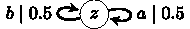
\includegraphics[width=91pt]{S3.Ex3.m1.g1.pdf}\end{center}
    \emph{It follows that %
% SOURCE HTML #S3.Thmtheorem4.p1.m16
\hypertarget{html:S3.Thmtheorem4.p1.m16}{}\({\left\llbracket{\mu v\leavevmode\nobreak\ (bv\oplus_{0.5}a(\mu u\leavevmode\nobreak\ (au\oplus_{0.5}bv))))}\right\rrbracket=\left\llbracket{\mu v\leavevmode\nobreak\ (av\oplus_{0.5}bv)}\right\rrbracket.}\)}
\par\medskip
    %
% SOURCE HTML #S3.SS0.SSS0.Px2
\hypertarget{html:S3.SS0.SSS0.Px2}{} \par\noindent\textbf{Axioms for stream equivalence}\quad  %
% SOURCE HTML #S3.SS0.SSS0.Px2.p1
\hypertarget{html:S3.SS0.SSS0.Px2.p1}{} As we have seen from \hyperlink{html:S3.Thmtheorem4}{Example 3.4}, even very different looking productive process terms can be stream equivalent. To facilitate reasoning about equivalence, we give a set of inference rules for deducing algebraically that two productive process terms are stream equivalent.
\par\medskip
  %
% SOURCE HTML #S3.Thmtheorem5
\hypertarget{html:S3.Thmtheorem5}{} \par\noindent\textbf{\textbf{Definition 3.5}\textbf{ }(Provable equivalence)\textbf{.}}\quad  %
% SOURCE HTML #S3.Thmtheorem5.p1
\hypertarget{html:S3.Thmtheorem5.p1}{} \emph{Probabilistic process terms %
% SOURCE HTML #S3.Thmtheorem5.p1.m1
\hypertarget{html:S3.Thmtheorem5.p1.m1}{}\({e,f\in\mathsf{PTerm}}\) are said to be \emph{provably equivalent}, written %
% SOURCE HTML #S3.Thmtheorem5.p1.m2
\hypertarget{html:S3.Thmtheorem5.p1.m2}{}\({e\equiv f}\), if %
% SOURCE HTML #S3.Thmtheorem5.p1.m3
\hypertarget{html:S3.Thmtheorem5.p1.m3}{}\({e=f}\) can be proven from axioms in \hyperlink{html:S3.F1}{Fig. 1}. We write %
% SOURCE HTML #S3.Thmtheorem5.p1.m4
\hypertarget{html:S3.Thmtheorem5.p1.m4}{}\({[e]}\) for the %
% SOURCE HTML #S3.Thmtheorem5.p1.m5
\hypertarget{html:S3.Thmtheorem5.p1.m5}{}\({\equiv}\)-equivalence class of %
% SOURCE HTML #S3.Thmtheorem5.p1.m6
\hypertarget{html:S3.Thmtheorem5.p1.m6}{}\({e}\).}
\par\medskip
   %
% SOURCE HTML #S3.F1
\hypertarget{html:S3.F1}{}
\begin{center}
 %
% SOURCE HTML #S8.EGx3
\hypertarget{html:S8.EGx3}{} %
% SOURCE HTML #S3.Ex10
\hypertarget{html:S3.Ex10}{}  %
% SOURCE HTML #S3.Ex10.m1
\hypertarget{html:S3.Ex10.m1}{}\[\displaystyle
\begin{aligned}
e&=e\oplus_r e\\
e_1\oplus_r e_2&=e_2\oplus_{1-r}e_1\\
(e_1\oplus_r e_2)\oplus_s e_3&=e_1\oplus_{rs}(e_2\oplus_{\frac{s(1-r)}{1-rs}}e_3)\\
a(e_1\oplus_r e_2)&=ae_1\oplus_r ae_2
\end{aligned}
\quad
\begin{gathered}
\mu v\,g=\mu u\,g[u/v]\\
\mu v\,g=g[\mu v\,g/v]\\
\frac{f=g[f/v]}{f=\mu v\,g}
\end{gathered}
\quad
\begin{gathered}
\frac{e_1=e_2}{ae_1=ae_2}\\[3pt]
\frac{e_1=f_1\quad e_2=f_2}{e_1\oplus_r e_2=f_1\oplus_r f_2}\\[3pt]
\frac{e_1=f_1\ \dots\ e_n=f_n}{k[\vec e/\vec v]=k[\vec f/\vec v]}
\end{gathered}
\]    
\par\smallskip Figure 1: Axioms for probabilistic term equivalence. Above, %
% SOURCE HTML #S3.F1.m12
\hypertarget{html:S3.F1.m12}{}\({e,e_{i},f,f_{i}\in\mathsf{PTerm}}\), %
% SOURCE HTML #S3.F1.m13
\hypertarget{html:S3.F1.m13}{}\({\vec{e}=(e_{1},\dots,e_{n})}\), %
% SOURCE HTML #S3.F1.m14
\hypertarget{html:S3.F1.m14}{}\({\vec{f}=(f_{1},\dots,f_{n})}\), %
% SOURCE HTML #S3.F1.m15
\hypertarget{html:S3.F1.m15}{}\({g\in\mathsf{PTerm}(v)}\), and %
% SOURCE HTML #S3.F1.m16
\hypertarget{html:S3.F1.m16}{}\({k\in\mathsf{PTerm}(v_{1},\dots,v_{n})}\). We assume that %
% SOURCE HTML #S3.F1.m17
\hypertarget{html:S3.F1.m17}{}\({u}\) is not bound in %
% SOURCE HTML #S3.F1.m18
\hypertarget{html:S3.F1.m18}{}\({g}\) in the first axiom of the second column. The term %
% SOURCE HTML #S3.F1.m19
\hypertarget{html:S3.F1.m19}{}\({k[\vec{e}/\vec{v}]}\) is obtained by simultaneously replacing %
% SOURCE HTML #S3.F1.m20
\hypertarget{html:S3.F1.m20}{}\({v_{i}}\) with %
% SOURCE HTML #S3.F1.m21
\hypertarget{html:S3.F1.m21}{}\({e_{i}}\) for each %
% SOURCE HTML #S3.F1.m22
\hypertarget{html:S3.F1.m22}{}\({i\leq n}\). Note that the equivalence relation axioms are implicit. The difference with the axiomatization for bisimilarity is the distributivity axiom (lower-left).
\par\medskip
 
\end{center}
 %
% SOURCE HTML #S3.SS0.SSS0.Px2.p2
\hypertarget{html:S3.SS0.SSS0.Px2.p2}{} The main goal of the paper is to prove that the axioms in \hyperlink{html:S3.F1}{Fig. 1} are sound and complete to reason about stream semantics of LMCs:
\par\medskip
 %
% SOURCE HTML #S3.Ex11
\hypertarget{html:S3.Ex11}{}   %
% SOURCE HTML #S3.Ex11.m1
\hypertarget{html:S3.Ex11.m1}{}\[e\equiv f\quad\Longleftrightarrow\quad\llbracket e\rrbracket=\llbracket f\rrbracket\qquad\qquad\qquad(\Longleftarrow):{\text{\footnotesize Completeness}}\qquad(\Longrightarrow):{\text{\footnotesize Soundness}}\]    Soundness was established in [\hyperlink{html:bib.bib21}{21}, Theorem 6.9]. The main result in this paper is completeness, which verifies [\hyperlink{html:bib.bib21}{21}, Conjecture 1].
\par\medskip
  %

% SOURCE HTML #S3.Thmtheorem6
\hypertarget{html:S3.Thmtheorem6}{} \par\noindent\textbf{\textbf{Theorem 3.6}\textbf{ }(Completeness)\textbf{.}}\quad  %
% SOURCE HTML #S3.Thmtheorem6.p1
\hypertarget{html:S3.Thmtheorem6.p1}{} \emph{Let %
% SOURCE HTML #S3.Thmtheorem6.p1.m1
\hypertarget{html:S3.Thmtheorem6.p1.m1}{}\({e,f\in\mathsf{PTerm}}\). If %
% SOURCE HTML #S3.Thmtheorem6.p1.m2
\hypertarget{html:S3.Thmtheorem6.p1.m2}{}\({\left\llbracket{e}\right\rrbracket=\left\llbracket{f}\right\rrbracket}\), then %
% SOURCE HTML #S3.Thmtheorem6.p1.m3
\hypertarget{html:S3.Thmtheorem6.p1.m3}{}\({e\equiv f}\).}
\par\medskip
    
%

% SOURCE HTML #S4
\hypertarget{html:S4}{} \section*{4 Blueprint for Proving Completeness}
 %
% SOURCE HTML #S4.p1
\hypertarget{html:S4.p1}{} The main goal of the rest of the paper is to prove \hyperlink{html:S3.Thmtheorem6}{Theorem 3.6}, completeness of our inference system. We begin with a high-level sketch of the proof to ease the flow into the upcoming technical sections. At the core of our argument will be the fact that the semantics of terms, as given by %
% SOURCE HTML #S4.p1.m1
\hypertarget{html:S4.p1.m1}{}\({\llbracket-\rrbracket}\), can be \emph{factorized}:
\par\medskip
 %
% SOURCE HTML #S4.E1
\hypertarget{html:S4.E1}{}   %
% SOURCE HTML #S4.E1.m1.g1
\hypertarget{html:S4.E1.m1.g1}{}\begin{center}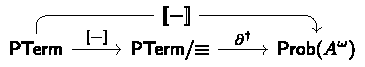
\includegraphics[width=175pt]{S4.E1.m1.g1.pdf}\end{center}
  (4.1)   The existence of this factorization is a consequence of soundness, which implies that %
% SOURCE HTML #S4.p1.m2
\hypertarget{html:S4.p1.m2}{}\({\left\llbracket{-}\right\rrbracket}\) factors through the quotient %
% SOURCE HTML #S4.p1.m3
\hypertarget{html:S4.p1.m3}{}\({\mathsf{PTerm}/{\equiv}}\) for a particular function %
% SOURCE HTML #S4.p1.m4
\hypertarget{html:S4.p1.m4}{}\({\partial^{\dagger}\colon\mathsf{PTerm}/{\equiv}\to\text{\sf Prob}(A^{\omega})}\). Once we have such factorization, we can reason as follows:
\par\medskip
 %
% SOURCE HTML #S8.EGx4
\hypertarget{html:S8.EGx4}{} %
% SOURCE HTML #S4.Ex1
\hypertarget{html:S4.Ex1}{}  %
% SOURCE HTML #S4.Ex1.m1
\hypertarget{html:S4.Ex1.m1}{}\({\displaystyle\left\llbracket{e}\right\rrbracket=\left\llbracket{f}\right\rrbracket\quad\Longrightarrow\quad\partial^{\dagger}([e])=\partial^{\dagger}([f])\quad\stackrel{{\scriptstyle\star}}{{\Longrightarrow}}\quad[e]=[f]\quad\Longrightarrow\quad e\equiv f}\)    Now completeness follows if we can justify the %
% SOURCE HTML #S4.p1.m5
\hypertarget{html:S4.p1.m5}{}\({\star}\) step, which amounts to injectivity of %
% SOURCE HTML #S4.p1.m6
\hypertarget{html:S4.p1.m6}{}\({\partial^{\dagger}}\). In other words, \hyperlink{html:S3.Thmtheorem6}{Theorem 3.6} follows if %
% SOURCE HTML #S4.p1.m7
\hypertarget{html:S4.p1.m7}{}\({\partial^{\dagger}}\) is injective. And that is precisely what we are going to prove. Before we outline the completeness proof, we need a few notions from convex algebra.
\par\medskip
  %
% SOURCE HTML #S4.Thmtheorem1
\hypertarget{html:S4.Thmtheorem1}{} \par\noindent\textbf{\textbf{Definition 4.1}\textbf{.}}\quad  %
% SOURCE HTML #S4.Thmtheorem1.p1
\hypertarget{html:S4.Thmtheorem1.p1}{} \emph{A \emph{convex algebra} is an algebraic structure consisting of a set %
% SOURCE HTML #S4.Thmtheorem1.p1.m1
\hypertarget{html:S4.Thmtheorem1.p1.m1}{}\({X}\) and a family of binary operations %
% SOURCE HTML #S4.Thmtheorem1.p1.m2
\hypertarget{html:S4.Thmtheorem1.p1.m2}{}\({\oplus_{p}\colon X\times X\to X}\) (written infix) satisfying}
\par\medskip
 %
% SOURCE HTML #S8.EGx5
\hypertarget{html:S8.EGx5}{} %
% SOURCE HTML #S4.Ex2
\hypertarget{html:S4.Ex2}{}  %
% SOURCE HTML #S4.Ex2.m1
\hypertarget{html:S4.Ex2.m1}{}\[\displaystyle x\oplus_{1}y=x\quad x\oplus_{r}x=x\quad x\oplus_{r}y=y\oplus_{1-r}x\quad(x\oplus_{r}y)\oplus_{s}z=x\oplus_{rs}\Big{(}y\oplus_{\frac{s(1-r)}{1-rs}}z\Big{)}\]    \emph{An \emph{affine map}, or \emph{convex algebra homomorphism}, between convex algebras %
% SOURCE HTML #S4.Thmtheorem1.p1.m3
\hypertarget{html:S4.Thmtheorem1.p1.m3}{}\({(X,\oplus^{X}_{p})}\) and %
% SOURCE HTML #S4.Thmtheorem1.p1.m4
\hypertarget{html:S4.Thmtheorem1.p1.m4}{}\({(Y,\oplus^{Y}_{p})}\) is a function %
% SOURCE HTML #S4.Thmtheorem1.p1.m5
\hypertarget{html:S4.Thmtheorem1.p1.m5}{}\({h\colon X\to Y}\) that satisfies %
% SOURCE HTML #S4.Thmtheorem1.p1.m6
\hypertarget{html:S4.Thmtheorem1.p1.m6}{}\({h(x\oplus^{X}_{p}y)=h(x)\oplus^{Y}_{p}h(y)}\) for each %
% SOURCE HTML #S4.Thmtheorem1.p1.m7
\hypertarget{html:S4.Thmtheorem1.p1.m7}{}\({p\in[0,1]}\). The category of convex algebras and affine maps is denoted %
% SOURCE HTML #S4.Thmtheorem1.p1.m8
\hypertarget{html:S4.Thmtheorem1.p1.m8}{}\({\mathsf{CA}}\).}
\par\medskip
  %
% SOURCE HTML #S4.Thmtheorem1.p2
\hypertarget{html:S4.Thmtheorem1.p2}{} \emph{A convex algebra %
% SOURCE HTML #S4.Thmtheorem1.p2.m1
\hypertarget{html:S4.Thmtheorem1.p2.m1}{}\({(X,\oplus^{X}_{p})}\) is \emph{free} and generated by a set %
% SOURCE HTML #S4.Thmtheorem1.p2.m2
\hypertarget{html:S4.Thmtheorem1.p2.m2}{}\({B\subseteq X}\) if every map %
% SOURCE HTML #S4.Thmtheorem1.p2.m3
\hypertarget{html:S4.Thmtheorem1.p2.m3}{}\({f\colon B\to Y}\) from %
% SOURCE HTML #S4.Thmtheorem1.p2.m4
\hypertarget{html:S4.Thmtheorem1.p2.m4}{}\({B}\) to the carrier of a convex algebra %
% SOURCE HTML #S4.Thmtheorem1.p2.m5
\hypertarget{html:S4.Thmtheorem1.p2.m5}{}\({(Y,\oplus^{Y}_{p})}\) extends to a unique affine map %
% SOURCE HTML #S4.Thmtheorem1.p2.m6
\hypertarget{html:S4.Thmtheorem1.p2.m6}{}\({f^{\#}\colon(X,\oplus^{X}_{p})\to(Y,\oplus^{Y}_{p})}\). The set %
% SOURCE HTML #S4.Thmtheorem1.p2.m7
\hypertarget{html:S4.Thmtheorem1.p2.m7}{}\({B}\) is then the set of generators of the free algebra %
% SOURCE HTML #S4.Thmtheorem1.p2.m8
\hypertarget{html:S4.Thmtheorem1.p2.m8}{}\({(X,\oplus^{X}_{p})}\). If %
% SOURCE HTML #S4.Thmtheorem1.p2.m9
\hypertarget{html:S4.Thmtheorem1.p2.m9}{}\({B}\) is a finite set, then the free algebra generated by %
% SOURCE HTML #S4.Thmtheorem1.p2.m10
\hypertarget{html:S4.Thmtheorem1.p2.m10}{}\({B}\) is \emph{free finitely generated}, \emph{ffg}, for short. A convex algebra is \emph{finitely generated}, \emph{fg}, for short, if it is a homomorphic image of a free finitely generated one.}
\par\medskip
   %
% SOURCE HTML #S4.p2
\hypertarget{html:S4.p2}{} Note that we will often write %
% SOURCE HTML #S4.p2.m1
\hypertarget{html:S4.p2.m1}{}\({X}\) instead of %
% SOURCE HTML #S4.p2.m2
\hypertarget{html:S4.p2.m2}{}\({(X,\oplus_{p})}\) if the convex algebra structure is clear from the context.
\par\medskip
  %
% SOURCE HTML #S4.p3
\hypertarget{html:S4.p3}{} Back to the intended completeness result as outlined above, we break the proof of injectivity of %
% SOURCE HTML #S4.p3.m1
\hypertarget{html:S4.p3.m1}{}\({\partial^{\dagger}}\) into 3 steps, each of independent interest.
\par\medskip
  %
% SOURCE HTML #S4.SS0.SSSx1
\hypertarget{html:S4.SS0.SSSx1}{} \par\noindent\textbf{Step 1}\quad  %
% SOURCE HTML #S4.SS0.SSSx1.p1
\hypertarget{html:S4.SS0.SSSx1.p1}{} We identify the category of convex algebras as the right base category to define the stream semantics of LMCs. More precisely, we define a functor %
% SOURCE HTML #S4.SS0.SSSx1.p1.m1
\hypertarget{html:S4.SS0.SSSx1.p1.m1}{}\({G}\) on %
% SOURCE HTML #S4.SS0.SSSx1.p1.m2
\hypertarget{html:S4.SS0.SSSx1.p1.m2}{}\({\mathsf{CA}}\) and show that the convex algebra of Borel probability distributions %
% SOURCE HTML #S4.SS0.SSSx1.p1.m3
\hypertarget{html:S4.SS0.SSSx1.p1.m3}{}\({\text{\sf Prob}(A^{\omega})}\) carries a final %
% SOURCE HTML #S4.SS0.SSSx1.p1.m4
\hypertarget{html:S4.SS0.SSSx1.p1.m4}{}\({G}\)-coalgebra structure %
% SOURCE HTML #S4.SS0.SSSx1.p1.m5
\hypertarget{html:S4.SS0.SSSx1.p1.m5}{}\({(\text{\sf Prob}(A^{\omega}),\zeta)}\). By turning any LMC %
% SOURCE HTML #S4.SS0.SSSx1.p1.m6
\hypertarget{html:S4.SS0.SSSx1.p1.m6}{}\({(X,\beta)}\) into a %
% SOURCE HTML #S4.SS0.SSSx1.p1.m7
\hypertarget{html:S4.SS0.SSSx1.p1.m7}{}\({G}\)-coalgebra %
% SOURCE HTML #S4.SS0.SSSx1.p1.m8
\hypertarget{html:S4.SS0.SSSx1.p1.m8}{}\({({\mathcal{D}}(X),\partial_{\beta})}\) via a \emph{determinization} construction (see \hyperlink{html:S5.Thmtheorem11}{Definition 5.11}), we obtain the \emph{determinized stream semantics} %
% SOURCE HTML #S4.SS0.SSSx1.p1.m9
\hypertarget{html:S4.SS0.SSSx1.p1.m9}{}\({(X,\beta)}\), %
% SOURCE HTML #S4.SS0.SSSx1.p1.m10
\hypertarget{html:S4.SS0.SSSx1.p1.m10}{}\({\llparenthesis{-}\rrparenthesis_{\beta}=\partial_{\beta}^{\dagger}\circ\eta\colon X\to{\mathcal{D}}(X)\to\text{\sf Prob}(A^{\omega})}\) via the final coalgebra homomorphism %
% SOURCE HTML #S4.SS0.SSSx1.p1.m11
\hypertarget{html:S4.SS0.SSSx1.p1.m11}{}\({\partial_{\beta}^{\dagger}\colon({\mathcal{D}}(X),\partial_{\beta})\to(\text{\sf Prob}(A^{\omega}),\zeta)}\). We then relate this determinized stream semantics to the original stream semantics %
% SOURCE HTML #S4.SS0.SSSx1.p1.m12
\hypertarget{html:S4.SS0.SSSx1.p1.m12}{}\({\left\llbracket{-}\right\rrbracket}\) defined in \hyperlink{html:S2.Thmtheorem3}{Proposition 2.3} using the syntactic LMC %
% SOURCE HTML #S4.SS0.SSSx1.p1.m13
\hypertarget{html:S4.SS0.SSSx1.p1.m13}{}\({(\mathsf{PTerm},\tau)}\) as shown in the diagram (\hyperlink{html:S4.E1}{4.1}).
\par\medskip
   %
% SOURCE HTML #S4.SS0.SSSx2
\hypertarget{html:S4.SS0.SSSx2}{} \par\noindent\textbf{Step 2}\quad  %
% SOURCE HTML #S4.SS0.SSSx2.p1
\hypertarget{html:S4.SS0.SSSx2.p1}{} We provide a %
% SOURCE HTML #S4.SS0.SSSx2.p1.m1
\hypertarget{html:S4.SS0.SSSx2.p1.m1}{}\({G}\)-coalgebra structure %
% SOURCE HTML #S4.SS0.SSSx2.p1.m2
\hypertarget{html:S4.SS0.SSSx2.p1.m2}{}\({(\mathsf{PTerm}/{\equiv},\partial)}\) on the equivalence classes of terms modulo provable equivalence and show that every ffg %
% SOURCE HTML #S4.SS0.SSSx2.p1.m3
\hypertarget{html:S4.SS0.SSSx2.p1.m3}{}\({G}\)-coalgebra %
% SOURCE HTML #S4.SS0.SSSx2.p1.m4
\hypertarget{html:S4.SS0.SSSx2.p1.m4}{}\({(X,\beta)}\) (i.e., %
% SOURCE HTML #S4.SS0.SSSx2.p1.m5
\hypertarget{html:S4.SS0.SSSx2.p1.m5}{}\({X}\) is ffg) has a unique coalgebra homomorphism into %
% SOURCE HTML #S4.SS0.SSSx2.p1.m6
\hypertarget{html:S4.SS0.SSSx2.p1.m6}{}\({(\mathsf{PTerm}/{\equiv},\partial)}\). This is related to solving certain systems of equations in %
% SOURCE HTML #S4.SS0.SSSx2.p1.m7
\hypertarget{html:S4.SS0.SSSx2.p1.m7}{}\({\mathsf{PTerm}/{\equiv}}\). We also show that %
% SOURCE HTML #S4.SS0.SSSx2.p1.m8
\hypertarget{html:S4.SS0.SSSx2.p1.m8}{}\({(\mathsf{PTerm}/{\equiv},\partial)}\) is \emph{locally fg}, in the following sense:
\par\medskip
  %
% SOURCE HTML #S4.Thmtheorem2
\hypertarget{html:S4.Thmtheorem2}{} \par\noindent\textbf{\textbf{Definition 4.2}\textbf{.}}\quad  %
% SOURCE HTML #S4.Thmtheorem2.p1
\hypertarget{html:S4.Thmtheorem2.p1}{} \emph{A %
% SOURCE HTML #S4.Thmtheorem2.p1.m1
\hypertarget{html:S4.Thmtheorem2.p1.m1}{}\({G}\)-coalgebra %
% SOURCE HTML #S4.Thmtheorem2.p1.m2
\hypertarget{html:S4.Thmtheorem2.p1.m2}{}\({(X,\gamma)}\) is \emph{locally fg} if for any %
% SOURCE HTML #S4.Thmtheorem2.p1.m3
\hypertarget{html:S4.Thmtheorem2.p1.m3}{}\({x\in X}\), there is a subcoalgebra %
% SOURCE HTML #S4.Thmtheorem2.p1.m4
\hypertarget{html:S4.Thmtheorem2.p1.m4}{}\({(U,\gamma_{U})}\) of %
% SOURCE HTML #S4.Thmtheorem2.p1.m5
\hypertarget{html:S4.Thmtheorem2.p1.m5}{}\({(X,\gamma)}\) such that %
% SOURCE HTML #S4.Thmtheorem2.p1.m6
\hypertarget{html:S4.Thmtheorem2.p1.m6}{}\({x\in U}\) and %
% SOURCE HTML #S4.Thmtheorem2.p1.m7
\hypertarget{html:S4.Thmtheorem2.p1.m7}{}\({U}\) is fg. A locally fg %
% SOURCE HTML #S4.Thmtheorem2.p1.m8
\hypertarget{html:S4.Thmtheorem2.p1.m8}{}\({G}\)-coalgebra %
% SOURCE HTML #S4.Thmtheorem2.p1.m9
\hypertarget{html:S4.Thmtheorem2.p1.m9}{}\({(X,\gamma)}\) is \emph{final} if every locally fg %
% SOURCE HTML #S4.Thmtheorem2.p1.m10
\hypertarget{html:S4.Thmtheorem2.p1.m10}{}\({G}\)-coalgebra admits a unique coalgebra homomorphism into %
% SOURCE HTML #S4.Thmtheorem2.p1.m11
\hypertarget{html:S4.Thmtheorem2.p1.m11}{}\({(X,\gamma)}\).}
\par\medskip
   %
% SOURCE HTML #S4.SS0.SSSx2.p2
\hypertarget{html:S4.SS0.SSSx2.p2}{} The significance of %
% SOURCE HTML #S4.SS0.SSSx2.p2.m1
\hypertarget{html:S4.SS0.SSSx2.p2.m1}{}\({(\mathsf{PTerm}/{\equiv},\partial)}\) being locally fg is related to the lemma below.
\par\medskip
  %
% SOURCE HTML #S4.Thmtheorem3
\hypertarget{html:S4.Thmtheorem3}{} \par\noindent\textbf{\textbf{Lemma 4.3}\textbf{.}}\quad  %
% SOURCE HTML #S4.Thmtheorem3.p1
\hypertarget{html:S4.Thmtheorem3.p1}{} \emph{Every homomorphic image of a locally fg %
% SOURCE HTML #S4.Thmtheorem3.p1.m1
\hypertarget{html:S4.Thmtheorem3.p1.m1}{}\({G}\)-coalgebra is also locally fg.}
\par\medskip
   %
% SOURCE HTML #S4.SS0.SSSx2.p3
\hypertarget{html:S4.SS0.SSSx2.p3}{} Consider the surjective-injective factorization of the coalgebra homomorphism %
% SOURCE HTML #S4.SS0.SSSx2.p3.m1
\hypertarget{html:S4.SS0.SSSx2.p3.m1}{}\({\partial^{\dagger}}\) below.
\par\medskip
 %
% SOURCE HTML #S4.Ex3
\hypertarget{html:S4.Ex3}{}   %
% SOURCE HTML #S4.Ex3.m1.g1
\hypertarget{html:S4.Ex3.m1.g1}{}\begin{center}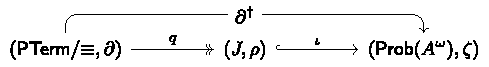
\includegraphics[width=235pt]{S4.Ex3.m1.g1.pdf}\end{center}
    To show that %
% SOURCE HTML #S4.SS0.SSSx2.p3.m2
\hypertarget{html:S4.SS0.SSSx2.p3.m2}{}\({\partial^{\dagger}}\) is injective, it suffices to show that the map %
% SOURCE HTML #S4.SS0.SSSx2.p3.m3
\hypertarget{html:S4.SS0.SSSx2.p3.m3}{}\({q}\) has a left inverse, a coalgebra homomorphism %
% SOURCE HTML #S4.SS0.SSSx2.p3.m4
\hypertarget{html:S4.SS0.SSSx2.p3.m4}{}\({k\colon(J,\rho)\to(\mathsf{PTerm}/{\equiv},\partial)}\) such that %
% SOURCE HTML #S4.SS0.SSSx2.p3.m5
\hypertarget{html:S4.SS0.SSSx2.p3.m5}{}\({k\circ q=\mathrm{id}}\), as then
\par\medskip
 %
% SOURCE HTML #S4.Ex4
\hypertarget{html:S4.Ex4}{}   %
% SOURCE HTML #S4.Ex4.m1
\hypertarget{html:S4.Ex4.m1}{}\[\partial^{\dagger}([e])=\partial^{\dagger}([f])\Leftrightarrow\iota\circ q([e])=\iota\circ q([f])\Rightarrow q([e])=q([f])\Rightarrow k\circ q([e])=k\circ q([f])\Leftrightarrow[e]=[f].\]    One way to do this is to show that %
% SOURCE HTML #S4.SS0.SSSx2.p3.m6
\hypertarget{html:S4.SS0.SSSx2.p3.m6}{}\({(\mathsf{PTerm}/{\equiv},\partial)}\) is the \emph{final} locally fg %
% SOURCE HTML #S4.SS0.SSSx2.p3.m7
\hypertarget{html:S4.SS0.SSSx2.p3.m7}{}\({G}\)-coalgebra. In such a case, by \hyperlink{html:S4.Thmtheorem3}{Lemma 4.3}, %
% SOURCE HTML #S4.SS0.SSSx2.p3.m8
\hypertarget{html:S4.SS0.SSSx2.p3.m8}{}\({(J,\rho)}\) is also locally fg, and therefore admits the desired (necessarily unique) coalgebra homomorphism %
% SOURCE HTML #S4.SS0.SSSx2.p3.m9
\hypertarget{html:S4.SS0.SSSx2.p3.m9}{}\({k}\). Indeed, by finality, since %
% SOURCE HTML #S4.SS0.SSSx2.p3.m10
\hypertarget{html:S4.SS0.SSSx2.p3.m10}{}\({k\circ q}\) and %
% SOURCE HTML #S4.SS0.SSSx2.p3.m11
\hypertarget{html:S4.SS0.SSSx2.p3.m11}{}\({\mathrm{id}}\) are both homomorphisms from %
% SOURCE HTML #S4.SS0.SSSx2.p3.m12
\hypertarget{html:S4.SS0.SSSx2.p3.m12}{}\({(\mathsf{PTerm}/{\equiv},\partial)}\) to itself, they must be the same, i.e., %
% SOURCE HTML #S4.SS0.SSSx2.p3.m13
\hypertarget{html:S4.SS0.SSSx2.p3.m13}{}\({k\circ q=\mathrm{id}}\).
\par\medskip
   %
% SOURCE HTML #S4.SS0.SSSx3
\hypertarget{html:S4.SS0.SSSx3}{} \par\noindent\textbf{Step 3}\quad  %
% SOURCE HTML #S4.SS0.SSSx3.p1
\hypertarget{html:S4.SS0.SSSx3.p1}{} Lastly, we will establish sufficient conditions guaranteeing that %
% SOURCE HTML #S4.SS0.SSSx3.p1.m1
\hypertarget{html:S4.SS0.SSSx3.p1.m1}{}\({(\mathsf{PTerm}/{\equiv},\partial)}\) is the final locally fg %
% SOURCE HTML #S4.SS0.SSSx3.p1.m2
\hypertarget{html:S4.SS0.SSSx3.p1.m2}{}\({G}\)-coalgebra. Our end goal will be to apply the following theorem, which can be obtained from a combination of [\hyperlink{html:bib.bib14}{14}, Corollary 5.9] and [\hyperlink{html:bib.bib27}{27}, Corollary 5.5].
\par\medskip
  %
% SOURCE HTML #S4.Thmtheorem4
\hypertarget{html:S4.Thmtheorem4}{} \par\noindent\textbf{\textbf{Theorem 4.4}\textbf{.}}\quad  %
% SOURCE HTML #S4.Thmtheorem4.p1
\hypertarget{html:S4.Thmtheorem4.p1}{} \emph{Suppose that %
% SOURCE HTML #S4.Thmtheorem4.p1.m1
\hypertarget{html:S4.Thmtheorem4.p1.m1}{}\({F}\) is a finitary proper endofunctor on %
% SOURCE HTML #S4.Thmtheorem4.p1.m2
\hypertarget{html:S4.Thmtheorem4.p1.m2}{}\({\mathsf{CA}}\) that preserves surjective affine maps. Then an %
% SOURCE HTML #S4.Thmtheorem4.p1.m3
\hypertarget{html:S4.Thmtheorem4.p1.m3}{}\({F}\)-coalgebra %
% SOURCE HTML #S4.Thmtheorem4.p1.m4
\hypertarget{html:S4.Thmtheorem4.p1.m4}{}\({(Y,\omega)}\) is a final locally fg coalgebra if and only if (i) %
% SOURCE HTML #S4.Thmtheorem4.p1.m5
\hypertarget{html:S4.Thmtheorem4.p1.m5}{}\({(Y,\omega)}\) is locally fg and (ii) for every ffg %
% SOURCE HTML #S4.Thmtheorem4.p1.m6
\hypertarget{html:S4.Thmtheorem4.p1.m6}{}\({F}\)-coalgebra %
% SOURCE HTML #S4.Thmtheorem4.p1.m7
\hypertarget{html:S4.Thmtheorem4.p1.m7}{}\({({\mathcal{D}}(X),\partial_{\beta})}\), there is a unique coalgebra homomorphism %
% SOURCE HTML #S4.Thmtheorem4.p1.m8
\hypertarget{html:S4.Thmtheorem4.p1.m8}{}\({({\mathcal{D}}(X),\partial_{\beta})\to(Y,\omega)}\).}
\par\medskip
   %
% SOURCE HTML #S4.SS0.SSSx3.p2
\hypertarget{html:S4.SS0.SSSx3.p2}{} \hyperlink{html:S4.Thmtheorem4}{Theorem 4.4} uses the notion of a \emph{proper} functor, which we will define in \hyperlink{html:S7.Thmtheorem6}{Definition 7.6} below.
\par\medskip
  %
% SOURCE HTML #S4.SS0.SSSx3.p3
\hypertarget{html:S4.SS0.SSSx3.p3}{} After having completed Step 2, we will have already seen that %
% SOURCE HTML #S4.SS0.SSSx3.p3.m1
\hypertarget{html:S4.SS0.SSSx3.p3.m1}{}\({(\mathsf{PTerm}/{\equiv},\partial)}\) is locally fg, and furthermore that every ffg %
% SOURCE HTML #S4.SS0.SSSx3.p3.m2
\hypertarget{html:S4.SS0.SSSx3.p3.m2}{}\({G}\)-coalgebra admits a unique coalgebra homomorphism into %
% SOURCE HTML #S4.SS0.SSSx3.p3.m3
\hypertarget{html:S4.SS0.SSSx3.p3.m3}{}\({(\mathsf{PTerm}/{\equiv},\partial)}\). Thus, completing Step 3 hinges on showing that the functor %
% SOURCE HTML #S4.SS0.SSSx3.p3.m4
\hypertarget{html:S4.SS0.SSSx3.p3.m4}{}\({G}\) is finitary, that it preserves surjective affine maps, and that %
% SOURCE HTML #S4.SS0.SSSx3.p3.m5
\hypertarget{html:S4.SS0.SSSx3.p3.m5}{}\({G}\) is proper. Step 3 is the most technical of the three steps. \newline{}To summarize, here are our obligations stated in the three steps above:
\par\medskip
 %
% SOURCE HTML #S4.I1
\hypertarget{html:S4.I1}{}
\begin{list}{}{\leftmargin=2em}
 %
% SOURCE HTML #S4.I1.i1
\hypertarget{html:S4.I1.i1}{}
\item[]  1. %
% SOURCE HTML #S4.I1.i1.p1
\hypertarget{html:S4.I1.i1.p1}{} We must define %
% SOURCE HTML #S4.I1.i1.p1.m1
\hypertarget{html:S4.I1.i1.p1.m1}{}\({G:\mathsf{CA}\to\mathsf{CA}}\), endow %
% SOURCE HTML #S4.I1.i1.p1.m2
\hypertarget{html:S4.I1.i1.p1.m2}{}\({\text{\sf Prob}(A^{\omega})}\) with a %
% SOURCE HTML #S4.I1.i1.p1.m3
\hypertarget{html:S4.I1.i1.p1.m3}{}\({G}\)-coalgebra structure %
% SOURCE HTML #S4.I1.i1.p1.m4
\hypertarget{html:S4.I1.i1.p1.m4}{}\({\zeta}\), turning %
% SOURCE HTML #S4.I1.i1.p1.m5
\hypertarget{html:S4.I1.i1.p1.m5}{}\({\text{\sf Prob}(A^{\omega},\zeta)}\) into a final %
% SOURCE HTML #S4.I1.i1.p1.m6
\hypertarget{html:S4.I1.i1.p1.m6}{}\({G}\)-coalgebra.
\par\medskip
  
 %
% SOURCE HTML #S4.I1.i2
\hypertarget{html:S4.I1.i2}{}
\item[]  2. %
% SOURCE HTML #S4.I1.i2.p1
\hypertarget{html:S4.I1.i2.p1}{} Given an LMC %
% SOURCE HTML #S4.I1.i2.p1.m1
\hypertarget{html:S4.I1.i2.p1.m1}{}\({(X,\beta)}\), we must explain how it is determinized to yield a %
% SOURCE HTML #S4.I1.i2.p1.m2
\hypertarget{html:S4.I1.i2.p1.m2}{}\({G}\)-coalgebra %
% SOURCE HTML #S4.I1.i2.p1.m3
\hypertarget{html:S4.I1.i2.p1.m3}{}\({(\mathcal{D}(X),\partial_{\beta})}\), and how its stream semantics %
% SOURCE HTML #S4.I1.i2.p1.m4
\hypertarget{html:S4.I1.i2.p1.m4}{}\({\left\llbracket{-}\right\rrbracket}\) is obtained from the final coalgebra homomorphism as %
% SOURCE HTML #S4.I1.i2.p1.m5
\hypertarget{html:S4.I1.i2.p1.m5}{}\({\left\llbracket{-}\right\rrbracket=\partial^{\dagger}_{\beta}\circ\eta}\). In other words, we must relate the stream semantics to the determinzed stream semantics %
% SOURCE HTML #S4.I1.i2.p1.m6
\hypertarget{html:S4.I1.i2.p1.m6}{}\({\llparenthesis{-}\rrparenthesis_{\beta}}\).
\par\medskip
  
 %
% SOURCE HTML #S4.I1.i3
\hypertarget{html:S4.I1.i3}{}
\item[]  3. %
% SOURCE HTML #S4.I1.i3.p1
\hypertarget{html:S4.I1.i3.p1}{} We must define a coalgebra structure %
% SOURCE HTML #S4.I1.i3.p1.m1
\hypertarget{html:S4.I1.i3.p1.m1}{}\({\partial:\mathsf{PTerm}/{\equiv}\to G(\mathsf{PTerm}/{\equiv})}\) and show that %
% SOURCE HTML #S4.I1.i3.p1.m2
\hypertarget{html:S4.I1.i3.p1.m2}{}\({(\mathsf{PTerm}/{\equiv},\partial)}\) is locally fg and that free fg %
% SOURCE HTML #S4.I1.i3.p1.m3
\hypertarget{html:S4.I1.i3.p1.m3}{}\({G}\)-coalgebras admit unique coalgebra homomorphisms into %
% SOURCE HTML #S4.I1.i3.p1.m4
\hypertarget{html:S4.I1.i3.p1.m4}{}\({(\mathsf{PTerm}/{\equiv},\partial)}\).
\par\medskip
  
 %
% SOURCE HTML #S4.I1.i4
\hypertarget{html:S4.I1.i4}{}
\item[]  4. %
% SOURCE HTML #S4.I1.i4.p1
\hypertarget{html:S4.I1.i4.p1}{} We must show that %
% SOURCE HTML #S4.I1.i4.p1.m1
\hypertarget{html:S4.I1.i4.p1.m1}{}\({G}\) is finitary, preserves surjective algebra homomorphisms, and is proper.
\par\medskip
  
 
\end{list}
   
%
% SOURCE HTML #S5
\hypertarget{html:S5}{} %
% SOURCE HTML #S5.m1
\hypertarget{html:S5.m1}{}\section*{5 Step 1: Convex (Co)Algebras and the Functor \({G}\)}
 %
% SOURCE HTML #S5.p1
\hypertarget{html:S5.p1}{} We begin executing each of the steps in \hyperlink{html:S4}{Section 4}. We first need some basic definitions on the category %
% SOURCE HTML #S5.p1.m1
\hypertarget{html:S5.p1.m1}{}\({\mathsf{CA}}\) of convex algebras.
\par\medskip
  %
% SOURCE HTML #S5.SS0.SSS0.P0.SPx1
\hypertarget{html:S5.SS0.SSS0.P0.SPx1}{} \par\noindent\textbf{Convex algebras.}\quad  %
% SOURCE HTML #S5.SS0.SSS0.P0.SPx1.p1
\hypertarget{html:S5.SS0.SSS0.P0.SPx1.p1}{} Recall that a \emph{convex algebra} is an algebraic structure consisting of a set %
% SOURCE HTML #S5.SS0.SSS0.P0.SPx1.p1.m1
\hypertarget{html:S5.SS0.SSS0.P0.SPx1.p1.m1}{}\({X}\) and a collection of \emph{convex sum operations} %
% SOURCE HTML #S5.SS0.SSS0.P0.SPx1.p1.m2
\hypertarget{html:S5.SS0.SSS0.P0.SPx1.p1.m2}{}\({\oplus_{r}\colon X\times X\to X}\) indexed by %
% SOURCE HTML #S5.SS0.SSS0.P0.SPx1.p1.m3
\hypertarget{html:S5.SS0.SSS0.P0.SPx1.p1.m3}{}\({r\in[0,1]}\) satisfying the equations in \hyperlink{html:S4.Thmtheorem1}{Definition 4.1}, and recall that we write %
% SOURCE HTML #S5.SS0.SSS0.P0.SPx1.p1.m4
\hypertarget{html:S5.SS0.SSS0.P0.SPx1.p1.m4}{}\({\mathsf{CA}}\) for the category of convex algebras.
\par\medskip
  %
% SOURCE HTML #S5.Thmtheorem1
\hypertarget{html:S5.Thmtheorem1}{} \par\noindent\textbf{\textbf{Example 5.1}\textbf{.}}\quad  %
% SOURCE HTML #S5.Thmtheorem1.p1
\hypertarget{html:S5.Thmtheorem1.p1}{} \emph{Prime examples of convex algebras are \emph{convex} subsets of %
% SOURCE HTML #S5.Thmtheorem1.p1.m1
\hypertarget{html:S5.Thmtheorem1.p1.m1}{}\({\mathbb{R}^{n}}\), i.e., subsets %
% SOURCE HTML #S5.Thmtheorem1.p1.m2
\hypertarget{html:S5.Thmtheorem1.p1.m2}{}\({C\subseteq\mathbb{R}^{n}}\) such that %
% SOURCE HTML #S5.Thmtheorem1.p1.m3
\hypertarget{html:S5.Thmtheorem1.p1.m3}{}\({\vec{p},\vec{q}\in C}\) implies that %
% SOURCE HTML #S5.Thmtheorem1.p1.m4
\hypertarget{html:S5.Thmtheorem1.p1.m4}{}\({\vec{p}\oplus_{r}\vec{q}=r\vec{p}+(1-r)\vec{q}\in C}\) for all %
% SOURCE HTML #S5.Thmtheorem1.p1.m5
\hypertarget{html:S5.Thmtheorem1.p1.m5}{}\({r\in[0,1]}\). Moreover, for any subset %
% SOURCE HTML #S5.Thmtheorem1.p1.m6
\hypertarget{html:S5.Thmtheorem1.p1.m6}{}\({U\subseteq\mathbb{R}^{n}}\), there is a smallest convex algebra containing %
% SOURCE HTML #S5.Thmtheorem1.p1.m7
\hypertarget{html:S5.Thmtheorem1.p1.m7}{}\({U}\), namely the \emph{convex hull} %
% SOURCE HTML #S5.Thmtheorem1.p1.m8
\hypertarget{html:S5.Thmtheorem1.p1.m8}{}\[\begin{aligned}\operatorname{conv}(U)&=\{r\vec{p}+(1-r)\vec{q}\\&\mid\vec{p},\vec{q}\in U\text{ and }r\in[0,1]\}\end{aligned}\].}
\par\medskip
   %
% SOURCE HTML #S5.SS0.SSS0.P0.SPx1.p2
\hypertarget{html:S5.SS0.SSS0.P0.SPx1.p2}{} We may use the following syntax as a generalized convex sum in an arbitrary convex algebra: given %
% SOURCE HTML #S5.SS0.SSS0.P0.SPx1.p2.m1
\hypertarget{html:S5.SS0.SSS0.P0.SPx1.p2.m1}{}\({r_{1},\dots,r_{n}\in(0,1)}\) and %
% SOURCE HTML #S5.SS0.SSS0.P0.SPx1.p2.m2
\hypertarget{html:S5.SS0.SSS0.P0.SPx1.p2.m2}{}\({x_{1},\dots,x_{n}}\), define
\par\medskip
 %
% SOURCE HTML #S5.E1
\hypertarget{html:S5.E1}{}   %
% SOURCE HTML #S5.E1.m1
\hypertarget{html:S5.E1.m1}{}\[\bigoplus_{i=1}^{n}r_{i}\cdot x_{i}=x_{n}\oplus_{r_{n}}\Big{(}\bigoplus_{i=1}^{n-1}\frac{r_{i}}{1-r_{n}}\cdot x_{i}\Big{)}\]  (5.1)   It is important to note that, technically, the base case is %
% SOURCE HTML #S5.SS0.SSS0.P0.SPx1.p2.m3
\hypertarget{html:S5.SS0.SSS0.P0.SPx1.p2.m3}{}\({n=2}\). We can also use this notation if %
% SOURCE HTML #S5.SS0.SSS0.P0.SPx1.p2.m4
\hypertarget{html:S5.SS0.SSS0.P0.SPx1.p2.m4}{}\({r_{i}=0}\) for %
% SOURCE HTML #S5.SS0.SSS0.P0.SPx1.p2.m5
\hypertarget{html:S5.SS0.SSS0.P0.SPx1.p2.m5}{}\({i\neq j}\) and %
% SOURCE HTML #S5.SS0.SSS0.P0.SPx1.p2.m6
\hypertarget{html:S5.SS0.SSS0.P0.SPx1.p2.m6}{}\({r_{j}=1}\), but in that case we define %
% SOURCE HTML #S5.SS0.SSS0.P0.SPx1.p2.m7
\hypertarget{html:S5.SS0.SSS0.P0.SPx1.p2.m7}{}\({\bigoplus_{i=1}^{n}r_{i}\cdot x_{i}=x_{j}}\). Up to the convex algebra axioms, any two ways of reordering the summands of (\hyperlink{html:S5.E1}{5.1}) produces equivalent terms. This justifies the slight abuse of notation %
% SOURCE HTML #S5.SS0.SSS0.P0.SPx1.p2.m8
\hypertarget{html:S5.SS0.SSS0.P0.SPx1.p2.m8}{}\({\bigoplus_{x\in S}r_{x}\cdot x}\), where %
% SOURCE HTML #S5.SS0.SSS0.P0.SPx1.p2.m9
\hypertarget{html:S5.SS0.SSS0.P0.SPx1.p2.m9}{}\({S}\) is a set and %
% SOURCE HTML #S5.SS0.SSS0.P0.SPx1.p2.m10
\hypertarget{html:S5.SS0.SSS0.P0.SPx1.p2.m10}{}\({r_{(-)}\colon S\to[0,1]}\) is a function such that %
% SOURCE HTML #S5.SS0.SSS0.P0.SPx1.p2.m11
\hypertarget{html:S5.SS0.SSS0.P0.SPx1.p2.m11}{}\({\sum_{x\in S}r_{x}=1}\) and only finitely many of the %
% SOURCE HTML #S5.SS0.SSS0.P0.SPx1.p2.m12
\hypertarget{html:S5.SS0.SSS0.P0.SPx1.p2.m12}{}\({r_{x}}\) are non-zero.
\par\medskip
   %
% SOURCE HTML #S5.SS0.SSS0.P0.SPx2
\hypertarget{html:S5.SS0.SSS0.P0.SPx2}{} \par\noindent\textbf{Free convex algebras.}\quad  %
% SOURCE HTML #S5.SS0.SSS0.P0.SPx2.p1
\hypertarget{html:S5.SS0.SSS0.P0.SPx2.p1}{} %
% SOURCE HTML #S5.SS0.SSS0.P0.SPx2.p1.m1
\hypertarget{html:S5.SS0.SSS0.P0.SPx2.p1.m1}{}\({({\mathcal{D}}(X),\oplus_{p})}\) is the \emph{free} convex algebra generated by the set %
% SOURCE HTML #S5.SS0.SSS0.P0.SPx2.p1.m2
\hypertarget{html:S5.SS0.SSS0.P0.SPx2.p1.m2}{}\({X}\). Hence, for any convex algebra %
% SOURCE HTML #S5.SS0.SSS0.P0.SPx2.p1.m3
\hypertarget{html:S5.SS0.SSS0.P0.SPx2.p1.m3}{}\({(Y,\oplus^{Y}_{p})}\), and any function %
% SOURCE HTML #S5.SS0.SSS0.P0.SPx2.p1.m4
\hypertarget{html:S5.SS0.SSS0.P0.SPx2.p1.m4}{}\({f\colon X\to Y}\), there is a unique \emph{linear extension} %
% SOURCE HTML #S5.SS0.SSS0.P0.SPx2.p1.m5
\hypertarget{html:S5.SS0.SSS0.P0.SPx2.p1.m5}{}\({f^{\#}\colon({\mathcal{D}}(X),\oplus_{p})\to(Y,\oplus^{Y}_{p})}\) of %
% SOURCE HTML #S5.SS0.SSS0.P0.SPx2.p1.m6
\hypertarget{html:S5.SS0.SSS0.P0.SPx2.p1.m6}{}\({f}\) such that %
% SOURCE HTML #S5.SS0.SSS0.P0.SPx2.p1.m7
\hypertarget{html:S5.SS0.SSS0.P0.SPx2.p1.m7}{}\({f^{\#}(1\cdot x)=f(x)}\). The universal property of free convex algebras gives rise to the adjunction %
% SOURCE HTML #S5.SS0.SSS0.P0.SPx2.p1.m8
\hypertarget{html:S5.SS0.SSS0.P0.SPx2.p1.m8}{}\({\mathcal{F}\dashv\mathcal{U}}\), where %
% SOURCE HTML #S5.SS0.SSS0.P0.SPx2.p1.m9
\hypertarget{html:S5.SS0.SSS0.P0.SPx2.p1.m9}{}\({{\mathcal{F}}(X)=({\mathcal{D}}(X),\oplus_{p})}\) is the \emph{free} functor that maps a set to the free convex algebra generated by it and a function %
% SOURCE HTML #S5.SS0.SSS0.P0.SPx2.p1.m10
\hypertarget{html:S5.SS0.SSS0.P0.SPx2.p1.m10}{}\({f\colon X\to Y}\) to %
% SOURCE HTML #S5.SS0.SSS0.P0.SPx2.p1.m11
\hypertarget{html:S5.SS0.SSS0.P0.SPx2.p1.m11}{}\({{\mathcal{D}}(f)\colon{\mathcal{D}}(X)\to{\mathcal{D}}(Y)}\), and %
% SOURCE HTML #S5.SS0.SSS0.P0.SPx2.p1.m12
\hypertarget{html:S5.SS0.SSS0.P0.SPx2.p1.m12}{}\({{\mathcal{U}}}\) is the \emph{forgetful} functor from %
% SOURCE HTML #S5.SS0.SSS0.P0.SPx2.p1.m13
\hypertarget{html:S5.SS0.SSS0.P0.SPx2.p1.m13}{}\({\mathsf{CA}}\) to %
% SOURCE HTML #S5.SS0.SSS0.P0.SPx2.p1.m14
\hypertarget{html:S5.SS0.SSS0.P0.SPx2.p1.m14}{}\({\mathsf{Set}}\) that forgets the algebraic structure and is identity on homomorphisms.
\par\medskip
  %
% SOURCE HTML #S5.SS0.SSS0.P0.SPx2.p2
\hypertarget{html:S5.SS0.SSS0.P0.SPx2.p2}{} The free functor %
% SOURCE HTML #S5.SS0.SSS0.P0.SPx2.p2.m1
\hypertarget{html:S5.SS0.SSS0.P0.SPx2.p2.m1}{}\({\mathcal{F}}\) is a left adjoint to the forgetful functor, and clearly %
% SOURCE HTML #S5.SS0.SSS0.P0.SPx2.p2.m2
\hypertarget{html:S5.SS0.SSS0.P0.SPx2.p2.m2}{}\({{\mathcal{D}}={\mathcal{U}}\circ{\mathcal{F}}}\). It follows that %
% SOURCE HTML #S5.SS0.SSS0.P0.SPx2.p2.m3
\hypertarget{html:S5.SS0.SSS0.P0.SPx2.p2.m3}{}\({({\mathcal{D}},\eta,\mu)}\) is a monad on %
% SOURCE HTML #S5.SS0.SSS0.P0.SPx2.p2.m4
\hypertarget{html:S5.SS0.SSS0.P0.SPx2.p2.m4}{}\({\mathsf{Set}}\) with %
% SOURCE HTML #S5.SS0.SSS0.P0.SPx2.p2.m5
\hypertarget{html:S5.SS0.SSS0.P0.SPx2.p2.m5}{}\({\eta_{X}(x)=1\cdot x}\) and %
% SOURCE HTML #S5.SS0.SSS0.P0.SPx2.p2.m6
\hypertarget{html:S5.SS0.SSS0.P0.SPx2.p2.m6}{}\({\mu_{X}=(\mathrm{id}_{{\mathcal{D}}(X)})^{\#}}\), and furthermore, %
% SOURCE HTML #S5.SS0.SSS0.P0.SPx2.p2.m7
\hypertarget{html:S5.SS0.SSS0.P0.SPx2.p2.m7}{}\({\mathsf{CA}}\) is isomorphic to the category of Eilenberg-Moore algebras for %
% SOURCE HTML #S5.SS0.SSS0.P0.SPx2.p2.m8
\hypertarget{html:S5.SS0.SSS0.P0.SPx2.p2.m8}{}\({{\mathcal{D}}}\) [\hyperlink{html:bib.bib31}{31}]. In particular, the free convex algebra generated by a set %
% SOURCE HTML #S5.SS0.SSS0.P0.SPx2.p2.m9
\hypertarget{html:S5.SS0.SSS0.P0.SPx2.p2.m9}{}\({X}\) is the Eilenberg-Moore algebra %
% SOURCE HTML #S5.SS0.SSS0.P0.SPx2.p2.m10
\hypertarget{html:S5.SS0.SSS0.P0.SPx2.p2.m10}{}\({({\mathcal{D}}(X),\mu_{X})}\). We often omit writing the forgetful functor when no confusion arises, and (in accordance with our convention to drop the algebra structure when no confusion arises) also often just write %
% SOURCE HTML #S5.SS0.SSS0.P0.SPx2.p2.m11
\hypertarget{html:S5.SS0.SSS0.P0.SPx2.p2.m11}{}\({{\mathcal{D}}(X)}\) for the free algebra %
% SOURCE HTML #S5.SS0.SSS0.P0.SPx2.p2.m12
\hypertarget{html:S5.SS0.SSS0.P0.SPx2.p2.m12}{}\({{\mathcal{F}}(X)}\).
\par\medskip
   %
% SOURCE HTML #S5.SS0.SSS0.P0.SPx3
\hypertarget{html:S5.SS0.SSS0.P0.SPx3}{} \par\noindent\textbf{Adding a fresh element %
% SOURCE HTML #S5.SS0.SSS0.P0.SPx3.m1
\hypertarget{html:S5.SS0.SSS0.P0.SPx3.m1}{}\({\bot}\) to a convex algebra.}\quad  %
% SOURCE HTML #S5.SS0.SSS0.P0.SPx3.p1
\hypertarget{html:S5.SS0.SSS0.P0.SPx3.p1}{} In order to define the endofunctor %
% SOURCE HTML #S5.SS0.SSS0.P0.SPx3.p1.m1
\hypertarget{html:S5.SS0.SSS0.P0.SPx3.p1.m1}{}\({G}\), we need the following construction on convex algebras. Given a convex algebra %
% SOURCE HTML #S5.SS0.SSS0.P0.SPx3.p1.m2
\hypertarget{html:S5.SS0.SSS0.P0.SPx3.p1.m2}{}\({X}\), define %
% SOURCE HTML #S5.SS0.SSS0.P0.SPx3.p1.m3
\hypertarget{html:S5.SS0.SSS0.P0.SPx3.p1.m3}{}\({X_{\bot}=\{\bot\}\cup\{r\cdot x\mid r\in(0,1],x\in X\}}\). The set %
% SOURCE HTML #S5.SS0.SSS0.P0.SPx3.p1.m4
\hypertarget{html:S5.SS0.SSS0.P0.SPx3.p1.m4}{}\({X_{\bot}}\) obtains a convex algebra structure with respect to the convex sum operation defined
\par\medskip
 %
% SOURCE HTML #S8.EGx6
\hypertarget{html:S8.EGx6}{} %
% SOURCE HTML #S5.Ex1
\hypertarget{html:S5.Ex1}{}  %
% SOURCE HTML #S5.Ex1.m1
\hypertarget{html:S5.Ex1.m1}{}\[\displaystyle\bot\oplus_{q}\bot=\bot\qquad r\cdot x\oplus_{q}\bot=(qr)\cdot x\qquad\bot\oplus_{q}s\cdot y=((1-q)s)\cdot y\]   %
% SOURCE HTML #S5.Ex2
\hypertarget{html:S5.Ex2}{}  %
% SOURCE HTML #S5.Ex2.m1
\hypertarget{html:S5.Ex2.m1}{}\[\displaystyle r\cdot x\oplus_{q}s\cdot y=(qr+(1-q)s)\cdot(x\oplus_{\frac{qr}{qr+(1-q)s}}y)\]     %
% SOURCE HTML #S5.Thmtheorem2
\hypertarget{html:S5.Thmtheorem2}{} \par\noindent\textbf{\textbf{Lemma 5.2}\textbf{.}}\quad  %
% SOURCE HTML #S5.Thmtheorem2.p1
\hypertarget{html:S5.Thmtheorem2.p1}{} \emph{Let %
% SOURCE HTML #S5.Thmtheorem2.p1.m1
\hypertarget{html:S5.Thmtheorem2.p1.m1}{}\({X}\) be a convex algebra. As defined above, %
% SOURCE HTML #S5.Thmtheorem2.p1.m2
\hypertarget{html:S5.Thmtheorem2.p1.m2}{}\({(X_{\bot},\oplus)}\) is a convex algebra. Moreover, given %
% SOURCE HTML #S5.Thmtheorem2.p1.m3
\hypertarget{html:S5.Thmtheorem2.p1.m3}{}\({r\cdot x}\) and %
% SOURCE HTML #S5.Thmtheorem2.p1.m4
\hypertarget{html:S5.Thmtheorem2.p1.m4}{}\({s\cdot y}\) in %
% SOURCE HTML #S5.Thmtheorem2.p1.m5
\hypertarget{html:S5.Thmtheorem2.p1.m5}{}\({X_{\bot}}\), %
% SOURCE HTML #S5.Thmtheorem2.p1.m6
\hypertarget{html:S5.Thmtheorem2.p1.m6}{}\({r\cdot x=s\cdot y}\) if and only if %
% SOURCE HTML #S5.Thmtheorem2.p1.m7
\hypertarget{html:S5.Thmtheorem2.p1.m7}{}\({r=s}\) and %
% SOURCE HTML #S5.Thmtheorem2.p1.m8
\hypertarget{html:S5.Thmtheorem2.p1.m8}{}\({x=y}\).}
\par\medskip
   %
% SOURCE HTML #S5.Thmtheorem3
\hypertarget{html:S5.Thmtheorem3}{} \par\noindent\textbf{%
% SOURCE HTML #S5.Thmtheorem3.m1
\hypertarget{html:S5.Thmtheorem3.m1}{}\({\blacktriangleright}\) Remark 5.3.}\quad  %
% SOURCE HTML #S5.Thmtheorem3.p1
\hypertarget{html:S5.Thmtheorem3.p1}{} \emph{We introduce some notation going forwards. We often use the notation %
% SOURCE HTML #S5.Thmtheorem3.p1.m1
\hypertarget{html:S5.Thmtheorem3.p1.m1}{}\({0\cdot x}\) for %
% SOURCE HTML #S5.Thmtheorem3.p1.m2
\hypertarget{html:S5.Thmtheorem3.p1.m2}{}\({\bot}\), even implicitly, despite that %
% SOURCE HTML #S5.Thmtheorem3.p1.m3
\hypertarget{html:S5.Thmtheorem3.p1.m3}{}\({0\cdot x=0\cdot y}\) for all %
% SOURCE HTML #S5.Thmtheorem3.p1.m4
\hypertarget{html:S5.Thmtheorem3.p1.m4}{}\({x,y\in X}\).}
\par\medskip
   %
% SOURCE HTML #S5.SS0.SSS0.P0.SPx3.p2
\hypertarget{html:S5.SS0.SSS0.P0.SPx3.p2}{} The construction %
% SOURCE HTML #S5.SS0.SSS0.P0.SPx3.p2.m1
\hypertarget{html:S5.SS0.SSS0.P0.SPx3.p2.m1}{}\({(-)_{\bot}\colon\mathsf{CA}\to\mathsf{CA}}\) is a functor whose action on convex algebra homomorphisms is given by %
% SOURCE HTML #S5.SS0.SSS0.P0.SPx3.p2.m2
\hypertarget{html:S5.SS0.SSS0.P0.SPx3.p2.m2}{}\({h_{\bot}(r\cdot x)=r\cdot h(x)}\) for any convex algebra homomorphism %
% SOURCE HTML #S5.SS0.SSS0.P0.SPx3.p2.m3
\hypertarget{html:S5.SS0.SSS0.P0.SPx3.p2.m3}{}\({h\colon(X,\oplus_{p})\to(Y,\oplus_{p})}\) and any %
% SOURCE HTML #S5.SS0.SSS0.P0.SPx3.p2.m4
\hypertarget{html:S5.SS0.SSS0.P0.SPx3.p2.m4}{}\({x\in X}\). The homomorphism %
% SOURCE HTML #S5.SS0.SSS0.P0.SPx3.p2.m5
\hypertarget{html:S5.SS0.SSS0.P0.SPx3.p2.m5}{}\({h_{\bot}}\) additionally satisfies %
% SOURCE HTML #S5.SS0.SSS0.P0.SPx3.p2.m6
\hypertarget{html:S5.SS0.SSS0.P0.SPx3.p2.m6}{}\({h_{\bot}(\bot)=\bot}\). Freely adjoining %
% SOURCE HTML #S5.SS0.SSS0.P0.SPx3.p2.m7
\hypertarget{html:S5.SS0.SSS0.P0.SPx3.p2.m7}{}\({\bot}\) is analogous to going from probability distributions to sub-probability distributions (maps %
% SOURCE HTML #S5.SS0.SSS0.P0.SPx3.p2.m8
\hypertarget{html:S5.SS0.SSS0.P0.SPx3.p2.m8}{}\({\theta\colon X\to[0,1]}\) such that %
% SOURCE HTML #S5.SS0.SSS0.P0.SPx3.p2.m9
\hypertarget{html:S5.SS0.SSS0.P0.SPx3.p2.m9}{}\({\sum_{x\in X}\theta(x)\leq 1}\)). The following lemma makes this precise.
\par\medskip
  %
% SOURCE HTML #S5.Thmtheorem4
\hypertarget{html:S5.Thmtheorem4}{} \par\noindent\textbf{\textbf{Lemma 5.4}\textbf{.}}\quad  %
% SOURCE HTML #S5.Thmtheorem4.p1
\hypertarget{html:S5.Thmtheorem4.p1}{} \emph{Let %
% SOURCE HTML #S5.Thmtheorem4.p1.m1
\hypertarget{html:S5.Thmtheorem4.p1.m1}{}\({{\mathcal{D}}_{\bot}}\) be the finitely supported sub-probability distribution functor, and let %
% SOURCE HTML #S5.Thmtheorem4.p1.m2
\hypertarget{html:S5.Thmtheorem4.p1.m2}{}\({\text{\sf Prob}_{\bot}(A^{\omega})}\) be the set of Borel sub-probability measures on %
% SOURCE HTML #S5.Thmtheorem4.p1.m3
\hypertarget{html:S5.Thmtheorem4.p1.m3}{}\({A^{\omega}}\). Then as convex algebras, %
% SOURCE HTML #S5.Thmtheorem4.p1.m4
\hypertarget{html:S5.Thmtheorem4.p1.m4}{}\({{\mathcal{D}}(X)_{\bot}\cong{\mathcal{D}}_{\bot}(X)}\) and %
% SOURCE HTML #S5.Thmtheorem4.p1.m5
\hypertarget{html:S5.Thmtheorem4.p1.m5}{}\({\text{\sf Prob}(A^{\omega})_{\bot}\cong\text{\sf Prob}_{\bot}(A^{\omega})}\).}
\par\medskip
    %
% SOURCE HTML #S5.SS0.SSS0.Px1
\hypertarget{html:S5.SS0.SSS0.Px1}{} \par\noindent\textbf{The functor %
% SOURCE HTML #S5.SS0.SSS0.Px1.m1
\hypertarget{html:S5.SS0.SSS0.Px1.m1}{}\({G:\mathsf{CA}\to\mathsf{CA}}\)}\quad  %
% SOURCE HTML #S5.SS0.SSS0.Px1.p1
\hypertarget{html:S5.SS0.SSS0.Px1.p1}{} We are now ready to introduce the functor on %
% SOURCE HTML #S5.SS0.SSS0.Px1.p1.m1
\hypertarget{html:S5.SS0.SSS0.Px1.p1.m1}{}\({\mathsf{CA}}\) needed to move from %
% SOURCE HTML #S5.SS0.SSS0.Px1.p1.m2
\hypertarget{html:S5.SS0.SSS0.Px1.p1.m2}{}\({\mathsf{Set}}\) to %
% SOURCE HTML #S5.SS0.SSS0.Px1.p1.m3
\hypertarget{html:S5.SS0.SSS0.Px1.p1.m3}{}\({\mathsf{CA}}\). There are different ways to define such a functor, e.g. Silva and Sokolova [\hyperlink{html:bib.bib25}{25}] use another functor for the axiomatization of finite trace semantics. The choice of the “right” functor so that our intended results go through, i.e., the choice of this particular functor %
% SOURCE HTML #S5.SS0.SSS0.Px1.p1.m4
\hypertarget{html:S5.SS0.SSS0.Px1.p1.m4}{}\({G}\), is one of the main contributions of this paper.
\par\medskip
  %
% SOURCE HTML #S5.SS0.SSS0.Px1.p2
\hypertarget{html:S5.SS0.SSS0.Px1.p2}{} Given a convex algebra %
% SOURCE HTML #S5.SS0.SSS0.Px1.p2.m1
\hypertarget{html:S5.SS0.SSS0.Px1.p2.m1}{}\({X}\) and a convex algebra homomorphism %
% SOURCE HTML #S5.SS0.SSS0.Px1.p2.m2
\hypertarget{html:S5.SS0.SSS0.Px1.p2.m2}{}\({h\colon X\to Y}\), let
\par\medskip
 %
% SOURCE HTML #S5.E2
\hypertarget{html:S5.E2}{}   %
% SOURCE HTML #S5.E2.m1
\hypertarget{html:S5.E2.m1}{}\[G(X)=\Big{\{}f:A\to X_{\bot}\,\mid\ \sum_{a\in A}r_{a}^{f}=1\Big{\}}\qquad G(h)(f)(a)=r_{a}^{f}\cdot h(x_{a}^{f})\]  (5.2)   where %
% SOURCE HTML #S5.SS0.SSS0.Px1.p2.m3
\hypertarget{html:S5.SS0.SSS0.Px1.p2.m3}{}\({f(a)=r_{a}^{f}\cdot x_{a}^{f}}\) for each %
% SOURCE HTML #S5.SS0.SSS0.Px1.p2.m4
\hypertarget{html:S5.SS0.SSS0.Px1.p2.m4}{}\({f\in G(X)}\) and %
% SOURCE HTML #S5.SS0.SSS0.Px1.p2.m5
\hypertarget{html:S5.SS0.SSS0.Px1.p2.m5}{}\({a\in A}\). Equivalently, %
% SOURCE HTML #S5.SS0.SSS0.Px1.p2.m6
\hypertarget{html:S5.SS0.SSS0.Px1.p2.m6}{}\({G(h)(f)=h_{\bot}\circ f}\). Note that in the definition of %
% SOURCE HTML #S5.SS0.SSS0.Px1.p2.m7
\hypertarget{html:S5.SS0.SSS0.Px1.p2.m7}{}\({G(X)}\) above, the sum is the usual sum of real numbers, and that we define %
% SOURCE HTML #S5.SS0.SSS0.Px1.p2.m8
\hypertarget{html:S5.SS0.SSS0.Px1.p2.m8}{}\({r_{a}^{f}=0}\) and leave %
% SOURCE HTML #S5.SS0.SSS0.Px1.p2.m9
\hypertarget{html:S5.SS0.SSS0.Px1.p2.m9}{}\({x_{a}^{f}}\) undefined when %
% SOURCE HTML #S5.SS0.SSS0.Px1.p2.m10
\hypertarget{html:S5.SS0.SSS0.Px1.p2.m10}{}\({f(a)=\bot}\).
\par\medskip
  %
% SOURCE HTML #S5.Thmtheorem5
\hypertarget{html:S5.Thmtheorem5}{} \par\noindent\textbf{\textbf{Proposition 5.5}\textbf{.}}\quad  %
% SOURCE HTML #S5.Thmtheorem5.p1
\hypertarget{html:S5.Thmtheorem5.p1}{} \emph{As it is defined in (\hyperlink{html:S5.E2}{5.2}), %
% SOURCE HTML #S5.Thmtheorem5.p1.m1
\hypertarget{html:S5.Thmtheorem5.p1.m1}{}\({G}\) is an endofunctor on %
% SOURCE HTML #S5.Thmtheorem5.p1.m2
\hypertarget{html:S5.Thmtheorem5.p1.m2}{}\({\mathsf{CA}}\).}
\par\medskip
   %
% SOURCE HTML #S5.SS0.SSS0.Px1.p3
\hypertarget{html:S5.SS0.SSS0.Px1.p3}{} We use the following terminology to refer to the defining property of %
% SOURCE HTML #S5.SS0.SSS0.Px1.p3.m1
\hypertarget{html:S5.SS0.SSS0.Px1.p3.m1}{}\({G}\): If %
% SOURCE HTML #S5.SS0.SSS0.Px1.p3.m2
\hypertarget{html:S5.SS0.SSS0.Px1.p3.m2}{}\({f:A\to X_{\bot}}\) has the property that %
% SOURCE HTML #S5.SS0.SSS0.Px1.p3.m3
\hypertarget{html:S5.SS0.SSS0.Px1.p3.m3}{}\({\sum_{a}r_{a}^{f}=1}\), as mentioned in (\hyperlink{html:S5.E2}{5.2}), we say that %
% SOURCE HTML #S5.SS0.SSS0.Px1.p3.m4
\hypertarget{html:S5.SS0.SSS0.Px1.p3.m4}{}\({f}\) satisfies the \emph{mass-splitting property}, or that %
% SOURCE HTML #S5.SS0.SSS0.Px1.p3.m5
\hypertarget{html:S5.SS0.SSS0.Px1.p3.m5}{}\({f}\) is \emph{mass splitting}.%
% SOURCE HTML #footnote1
\hypertarget{html:footnote1}{}\footnote{The mass-splitting property was inspired by a condition in Goy and Rot’s paper [\hyperlink{html:bib.bib6}{6}, Proposition 4.5].}
\par\medskip
  %
% SOURCE HTML #S5.SS0.SSS0.Px1.p4
\hypertarget{html:S5.SS0.SSS0.Px1.p4}{} In particular, a function %
% SOURCE HTML #S5.SS0.SSS0.Px1.p4.m1
\hypertarget{html:S5.SS0.SSS0.Px1.p4.m1}{}\({f\colon A\to{\mathcal{D}}_{\bot}(X)}\) is mass splitting, i.e., %
% SOURCE HTML #S5.SS0.SSS0.Px1.p4.m2
\hypertarget{html:S5.SS0.SSS0.Px1.p4.m2}{}\({f\in G({\mathcal{D}}(X))}\), if and only if the total mass %
% SOURCE HTML #S5.SS0.SSS0.Px1.p4.m3
\hypertarget{html:S5.SS0.SSS0.Px1.p4.m3}{}\({\sum_{a\in A}\sum_{x\in X}f(a)(x)}\) is equal to %
% SOURCE HTML #S5.SS0.SSS0.Px1.p4.m4
\hypertarget{html:S5.SS0.SSS0.Px1.p4.m4}{}\({1}\). Given such a function, one can reverse-engineer a unique probability distribution %
% SOURCE HTML #S5.SS0.SSS0.Px1.p4.m5
\hypertarget{html:S5.SS0.SSS0.Px1.p4.m5}{}\({\theta\in{\mathcal{D}}(A\times X)}\) such that %
% SOURCE HTML #S5.SS0.SSS0.Px1.p4.m6
\hypertarget{html:S5.SS0.SSS0.Px1.p4.m6}{}\({f}\) computes the marginal %
% SOURCE HTML #S5.SS0.SSS0.Px1.p4.m7
\hypertarget{html:S5.SS0.SSS0.Px1.p4.m7}{}\({f(a)=\theta(\{a\}\times X)}\) for each %
% SOURCE HTML #S5.SS0.SSS0.Px1.p4.m8
\hypertarget{html:S5.SS0.SSS0.Px1.p4.m8}{}\({a\in A}\). Thus, a %
% SOURCE HTML #S5.SS0.SSS0.Px1.p4.m9
\hypertarget{html:S5.SS0.SSS0.Px1.p4.m9}{}\({G}\)-coalgebra of the form %
% SOURCE HTML #S5.SS0.SSS0.Px1.p4.m10
\hypertarget{html:S5.SS0.SSS0.Px1.p4.m10}{}\({({\mathcal{D}}(X),\gamma)}\) represents the same data as an LMC %
% SOURCE HTML #S5.SS0.SSS0.Px1.p4.m11
\hypertarget{html:S5.SS0.SSS0.Px1.p4.m11}{}\({(X,\beta)}\) by reverse-engineering %
% SOURCE HTML #S5.SS0.SSS0.Px1.p4.m12
\hypertarget{html:S5.SS0.SSS0.Px1.p4.m12}{}\({\beta(x)}\) from %
% SOURCE HTML #S5.SS0.SSS0.Px1.p4.m13
\hypertarget{html:S5.SS0.SSS0.Px1.p4.m13}{}\({\gamma(1\cdot x)}\) for each %
% SOURCE HTML #S5.SS0.SSS0.Px1.p4.m14
\hypertarget{html:S5.SS0.SSS0.Px1.p4.m14}{}\({x\in X}\). We think of %
% SOURCE HTML #S5.SS0.SSS0.Px1.p4.m15
\hypertarget{html:S5.SS0.SSS0.Px1.p4.m15}{}\({G}\)-coalgebras as the \emph{deterministic} counterpart of LMCs. Their exact relationship will be made precise at the end of this section.
\par\medskip
  %
% SOURCE HTML #S5.Thmtheorem6
\hypertarget{html:S5.Thmtheorem6}{} \par\noindent\textbf{%
% SOURCE HTML #S5.Thmtheorem6.m1
\hypertarget{html:S5.Thmtheorem6.m1}{}\({\blacktriangleright}\) Remark 5.6.}\quad  %
% SOURCE HTML #S5.Thmtheorem6.p1
\hypertarget{html:S5.Thmtheorem6.p1}{} \emph{Note that as a set, %
% SOURCE HTML #S5.Thmtheorem6.p1.m1
\hypertarget{html:S5.Thmtheorem6.p1.m1}{}\({X_{\bot}\cong 1+(0,1]\times X}\), and so the description of %
% SOURCE HTML #S5.Thmtheorem6.p1.m2
\hypertarget{html:S5.Thmtheorem6.p1.m2}{}\({G(X)}\) above can also be taken as a definition of a functor %
% SOURCE HTML #S5.Thmtheorem6.p1.m3
\hypertarget{html:S5.Thmtheorem6.p1.m3}{}\({H\colon\mathsf{Set}\to\mathsf{Set}}\). Indeed, %
% SOURCE HTML #S5.Thmtheorem6.p1.m4
\hypertarget{html:S5.Thmtheorem6.p1.m4}{}\({G}\) is a lifting of %
% SOURCE HTML #S5.Thmtheorem6.p1.m5
\hypertarget{html:S5.Thmtheorem6.p1.m5}{}\({H}\) to %
% SOURCE HTML #S5.Thmtheorem6.p1.m6
\hypertarget{html:S5.Thmtheorem6.p1.m6}{}\({\mathsf{CA}}\). However, the convex algebra structure on %
% SOURCE HTML #S5.Thmtheorem6.p1.m7
\hypertarget{html:S5.Thmtheorem6.p1.m7}{}\({X_{\bot}}\) is not the convex algebra structure on %
% SOURCE HTML #S5.Thmtheorem6.p1.m8
\hypertarget{html:S5.Thmtheorem6.p1.m8}{}\({1+(0,1]\times X}\) obtained from (co)products in %
% SOURCE HTML #S5.Thmtheorem6.p1.m9
\hypertarget{html:S5.Thmtheorem6.p1.m9}{}\({\mathsf{CA}}\). The convex algebra structure is instead hand-tailored to match the structure of sub-probability distributions.}
\par\medskip
   %
% SOURCE HTML #S5.SS0.SSS0.Px1.p5
\hypertarget{html:S5.SS0.SSS0.Px1.p5}{} In a given %
% SOURCE HTML #S5.SS0.SSS0.Px1.p5.m1
\hypertarget{html:S5.SS0.SSS0.Px1.p5.m1}{}\({G}\)-coalgebra %
% SOURCE HTML #S5.SS0.SSS0.Px1.p5.m2
\hypertarget{html:S5.SS0.SSS0.Px1.p5.m2}{}\({(X,\gamma)}\), we write %
% SOURCE HTML #S5.SS0.SSS0.Px1.p5.m3
\hypertarget{html:S5.SS0.SSS0.Px1.p5.m3}{}\({\mbox{\sf mass}_{\gamma}(a,x)}\) for %
% SOURCE HTML #S5.SS0.SSS0.Px1.p5.m4
\hypertarget{html:S5.SS0.SSS0.Px1.p5.m4}{}\({r_{a}^{\gamma(x)}}\), and whenever %
% SOURCE HTML #S5.SS0.SSS0.Px1.p5.m5
\hypertarget{html:S5.SS0.SSS0.Px1.p5.m5}{}\({r_{a}^{\gamma(x)}>0}\), we write %
% SOURCE HTML #S5.SS0.SSS0.Px1.p5.m6
\hypertarget{html:S5.SS0.SSS0.Px1.p5.m6}{}\({\mbox{\sf next}_{\gamma}(a,x)}\) for %
% SOURCE HTML #S5.SS0.SSS0.Px1.p5.m7
\hypertarget{html:S5.SS0.SSS0.Px1.p5.m7}{}\({x_{a}^{\gamma(x)}}\). Then whenever %
% SOURCE HTML #S5.SS0.SSS0.Px1.p5.m8
\hypertarget{html:S5.SS0.SSS0.Px1.p5.m8}{}\({\gamma(x)(a)=\bot}\), %
% SOURCE HTML #S5.SS0.SSS0.Px1.p5.m9
\hypertarget{html:S5.SS0.SSS0.Px1.p5.m9}{}\({\mbox{\sf mass}_{\gamma}(a,x)=0}\) while %
% SOURCE HTML #S5.SS0.SSS0.Px1.p5.m10
\hypertarget{html:S5.SS0.SSS0.Px1.p5.m10}{}\({\mbox{\sf next}_{\gamma}(a,x)}\) is undefined; and when %
% SOURCE HTML #S5.SS0.SSS0.Px1.p5.m11
\hypertarget{html:S5.SS0.SSS0.Px1.p5.m11}{}\({\mbox{\sf mass}_{\gamma}(a,x)>0}\),
\par\medskip
 %
% SOURCE HTML #S5.E3
\hypertarget{html:S5.E3}{}   %
% SOURCE HTML #S5.E3.m1
\hypertarget{html:S5.E3.m1}{}\[\gamma(x)(a)=\mbox{\sf mass}_{\gamma}(a,x)\cdot\mbox{\sf next}_{\gamma}(a,x).\]  (5.3)   where the %
% SOURCE HTML #S5.SS0.SSS0.Px1.p5.m12
\hypertarget{html:S5.SS0.SSS0.Px1.p5.m12}{}\({\cdot}\) symbol here is from %
% SOURCE HTML #S5.SS0.SSS0.Px1.p5.m13
\hypertarget{html:S5.SS0.SSS0.Px1.p5.m13}{}\({X_{\bot}}\). Note that we often drop %
% SOURCE HTML #S5.SS0.SSS0.Px1.p5.m14
\hypertarget{html:S5.SS0.SSS0.Px1.p5.m14}{}\({\gamma}\) and write simply mass and next. In this notation, the mass-splitting property says that for all %
% SOURCE HTML #S5.SS0.SSS0.Px1.p5.m17
\hypertarget{html:S5.SS0.SSS0.Px1.p5.m17}{}\({x\in X}\), we have %
% SOURCE HTML #S5.SS0.SSS0.Px1.p5.m18
\hypertarget{html:S5.SS0.SSS0.Px1.p5.m18}{}\({\sum_{a\in A}\mbox{\sf mass}(a,x)=1}\).
\par\medskip
  %
% SOURCE HTML #S5.SS0.SSS0.Px1.p6
\hypertarget{html:S5.SS0.SSS0.Px1.p6}{} Given %
% SOURCE HTML #S5.SS0.SSS0.Px1.p6.m1
\hypertarget{html:S5.SS0.SSS0.Px1.p6.m1}{}\({G}\)-coalgebras %
% SOURCE HTML #S5.SS0.SSS0.Px1.p6.m2
\hypertarget{html:S5.SS0.SSS0.Px1.p6.m2}{}\({(X,\gamma)}\) and %
% SOURCE HTML #S5.SS0.SSS0.Px1.p6.m3
\hypertarget{html:S5.SS0.SSS0.Px1.p6.m3}{}\({(Y,\omega)}\), unravelling the definitions of mass and next reveals that a function %
% SOURCE HTML #S5.SS0.SSS0.Px1.p6.m6
\hypertarget{html:S5.SS0.SSS0.Px1.p6.m6}{}\({h:X\to Y}\) is a coalgebra homomorphism if and only if
\par\medskip
 %
% SOURCE HTML #S5.E4
\hypertarget{html:S5.E4}{}   %
% SOURCE HTML #S5.E4.m1
\hypertarget{html:S5.E4.m1}{}\[\mbox{\sf mass}(a,x)\cdot h(\mbox{\sf next}(a,x))=\mbox{\sf mass}(a,h(x))\cdot\mbox{\sf next}(a,h(x))\]  (5.4)   for any %
% SOURCE HTML #S5.SS0.SSS0.Px1.p6.m7
\hypertarget{html:S5.SS0.SSS0.Px1.p6.m7}{}\({a\in A}\) and %
% SOURCE HTML #S5.SS0.SSS0.Px1.p6.m8
\hypertarget{html:S5.SS0.SSS0.Px1.p6.m8}{}\({x\in X}\). In other words, for all %
% SOURCE HTML #S5.SS0.SSS0.Px1.p6.m9
\hypertarget{html:S5.SS0.SSS0.Px1.p6.m9}{}\({x\in X}\) and %
% SOURCE HTML #S5.SS0.SSS0.Px1.p6.m10
\hypertarget{html:S5.SS0.SSS0.Px1.p6.m10}{}\({a\in A}\), %
% SOURCE HTML #S5.SS0.SSS0.Px1.p6.m11
\hypertarget{html:S5.SS0.SSS0.Px1.p6.m11}{}\({\mbox{\sf mass}(a,x)=\mbox{\sf mass}(a,h(x))}\), and if this is greater than %
% SOURCE HTML #S5.SS0.SSS0.Px1.p6.m12
\hypertarget{html:S5.SS0.SSS0.Px1.p6.m12}{}\({0}\), then %
% SOURCE HTML #S5.SS0.SSS0.Px1.p6.m13
\hypertarget{html:S5.SS0.SSS0.Px1.p6.m13}{}\({h(\mbox{\sf next}(a,x))=\mbox{\sf next}(a,h(x))}\) as well.
\par\medskip
  %
% SOURCE HTML #S5.SS0.SSS0.Px1.SPx1
\hypertarget{html:S5.SS0.SSS0.Px1.SPx1}{} \par\noindent\textbf{A final %
% SOURCE HTML #S5.SS0.SSS0.Px1.SPx1.m1
\hypertarget{html:S5.SS0.SSS0.Px1.SPx1.m1}{}\({G}\)-coalgebra.}\quad  %
% SOURCE HTML #S5.SS0.SSS0.Px1.SPx1.p1
\hypertarget{html:S5.SS0.SSS0.Px1.SPx1.p1}{} We are now in the position to show that %
% SOURCE HTML #S5.SS0.SSS0.Px1.SPx1.p1.m1
\hypertarget{html:S5.SS0.SSS0.Px1.SPx1.p1.m1}{}\({\text{\sf Prob}(A^{\omega})}\) is the carrier of a final %
% SOURCE HTML #S5.SS0.SSS0.Px1.SPx1.p1.m2
\hypertarget{html:S5.SS0.SSS0.Px1.SPx1.p1.m2}{}\({G}\)-coalgebra. First, observe that, like %
% SOURCE HTML #S5.SS0.SSS0.Px1.SPx1.p1.m3
\hypertarget{html:S5.SS0.SSS0.Px1.SPx1.p1.m3}{}\({{\mathcal{D}}(X)}\), %
% SOURCE HTML #S5.SS0.SSS0.Px1.SPx1.p1.m4
\hypertarget{html:S5.SS0.SSS0.Px1.SPx1.p1.m4}{}\({\text{\sf Prob}(A^{\omega})}\) is a convex algebra with the canonical convex sums, %
% SOURCE HTML #S5.SS0.SSS0.Px1.SPx1.p1.m5
\hypertarget{html:S5.SS0.SSS0.Px1.SPx1.p1.m5}{}\({\rho\oplus_{r}\theta=r\rho+(1-r)\theta}\). In the proof of \hyperlink{html:S5.Thmtheorem13}{Theorem 5.13}, we use the %
% SOURCE HTML #S5.SS0.SSS0.Px1.SPx1.p1.m6
\hypertarget{html:S5.SS0.SSS0.Px1.SPx1.p1.m6}{}\({{\mathcal{D}}}\)-algebra in the more general, Eilenberg-Moore, form %
% SOURCE HTML #S5.SS0.SSS0.Px1.SPx1.p1.m7
\hypertarget{html:S5.SS0.SSS0.Px1.SPx1.p1.m7}{}\({(\text{\sf Prob}(A^{\omega}),\Sigma)}\), where
\par\medskip
 %
% SOURCE HTML #S5.E5
\hypertarget{html:S5.E5}{}   %
% SOURCE HTML #S5.E5.m1
\hypertarget{html:S5.E5.m1}{}\[\Sigma(\sum\limits_{i=1}^{n}r_{i}\cdot\rho_{i})(B)=\sum\limits_{i=1}^{n}r_{i}\rho_{i}(B)\]  (5.5)    %
% SOURCE HTML #S5.Thmtheorem7
\hypertarget{html:S5.Thmtheorem7}{} \par\noindent\textbf{\textbf{Definition 5.7}\textbf{.}}\quad  %
% SOURCE HTML #S5.Thmtheorem7.p1
\hypertarget{html:S5.Thmtheorem7.p1}{} \emph{The %
% SOURCE HTML #S5.Thmtheorem7.p1.m1
\hypertarget{html:S5.Thmtheorem7.p1.m1}{}\({G}\)-coalgebra structure %
% SOURCE HTML #S5.Thmtheorem7.p1.m2
\hypertarget{html:S5.Thmtheorem7.p1.m2}{}\({(\text{\sf Prob}(A^{\omega}),\zeta)}\) is given by, for %
% SOURCE HTML #S5.Thmtheorem7.p1.m3
\hypertarget{html:S5.Thmtheorem7.p1.m3}{}\({\rho\in\text{\sf Prob}(A^{\omega})}\),}
\par\medskip
 %
% SOURCE HTML #S5.E6
\hypertarget{html:S5.E6}{}   %
% SOURCE HTML #S5.E6.m1
\hypertarget{html:S5.E6.m1}{}\[\zeta(\rho)(a)=\left\{\begin{array}[]{ll}\bot&\mbox{if $\rho(B_{a})=0$}\\
\rho(B_{a})\cdot\big{(}B\mapsto\rho(aB)/\rho(B_{a})\big{)}&\mbox{if $\rho(B_{a})>0$}\end{array}\right.\]  (5.6)   \emph{where for Borel %
% SOURCE HTML #S5.Thmtheorem7.p1.m4
\hypertarget{html:S5.Thmtheorem7.p1.m4}{}\({B}\), %
% SOURCE HTML #S5.Thmtheorem7.p1.m5
\hypertarget{html:S5.Thmtheorem7.p1.m5}{}\({aB=\{(a,a_{1},\dots)\mid(a_{1},\dots)\in B\}}\) is the Borel set obtained by prefixing.}
\par\medskip
   %
% SOURCE HTML #S5.SS0.SSS0.Px1.SPx1.p2
\hypertarget{html:S5.SS0.SSS0.Px1.SPx1.p2}{} It is easy to check that %
% SOURCE HTML #S5.SS0.SSS0.Px1.SPx1.p2.m1
\hypertarget{html:S5.SS0.SSS0.Px1.SPx1.p2.m1}{}\({\zeta}\) is a convex algebra homomorphism and that %
% SOURCE HTML #S5.SS0.SSS0.Px1.SPx1.p2.m2
\hypertarget{html:S5.SS0.SSS0.Px1.SPx1.p2.m2}{}\({\zeta(\rho)}\) satisfies the mass-splitting property for each %
% SOURCE HTML #S5.SS0.SSS0.Px1.SPx1.p2.m3
\hypertarget{html:S5.SS0.SSS0.Px1.SPx1.p2.m3}{}\({\rho\in\text{\sf Prob}(A^{\omega})}\).
\par\medskip
  %
% SOURCE HTML #S5.Thmtheorem8
\hypertarget{html:S5.Thmtheorem8}{} \par\noindent\textbf{%
% SOURCE HTML #S5.Thmtheorem8.m1
\hypertarget{html:S5.Thmtheorem8.m1}{}\({\blacktriangleright}\) Remark 5.8.}\quad  %
% SOURCE HTML #S5.Thmtheorem8.p1
\hypertarget{html:S5.Thmtheorem8.p1}{} \emph{It is important to note that %
% SOURCE HTML #S5.Thmtheorem8.p1.m1
\hypertarget{html:S5.Thmtheorem8.p1.m1}{}\({\mbox{\sf next}_{\zeta}(a,-)\colon\text{\sf Prob}(A^{\omega})\to\text{\sf Prob}(A^{\omega})}\) is \emph{not} (in general) a convex algebra homomorphism.}
\par\medskip
   %
% SOURCE HTML #S5.Thmtheorem9
\hypertarget{html:S5.Thmtheorem9}{} \par\noindent\textbf{\textbf{Theorem 5.9}\textbf{.}}\quad  %
% SOURCE HTML #S5.Thmtheorem9.p1
\hypertarget{html:S5.Thmtheorem9.p1}{} \emph{The %
% SOURCE HTML #S5.Thmtheorem9.p1.m1
\hypertarget{html:S5.Thmtheorem9.p1.m1}{}\({G}\)-coalgebra %
% SOURCE HTML #S5.Thmtheorem9.p1.m2
\hypertarget{html:S5.Thmtheorem9.p1.m2}{}\({(\text{\sf Prob}(A^{\omega}),\zeta)}\) is final. That is, for any %
% SOURCE HTML #S5.Thmtheorem9.p1.m3
\hypertarget{html:S5.Thmtheorem9.p1.m3}{}\({G}\)-coalgebra %
% SOURCE HTML #S5.Thmtheorem9.p1.m4
\hypertarget{html:S5.Thmtheorem9.p1.m4}{}\({(X,\gamma)}\), there is a unique coalgebra homomorphism %
% SOURCE HTML #S5.Thmtheorem9.p1.m5
\hypertarget{html:S5.Thmtheorem9.p1.m5}{}\({\gamma^{{\dagger}}\colon(X,\gamma)\to(\text{\sf Prob}(A^{\omega}),\zeta)}\).}
\par\medskip
   %
% SOURCE HTML #S5.SS0.SSS0.Px1.SPx1.p3
\hypertarget{html:S5.SS0.SSS0.Px1.SPx1.p3}{} Here is a hint of a hint. We define %
% SOURCE HTML #S5.SS0.SSS0.Px1.SPx1.p3.m1
\hypertarget{html:S5.SS0.SSS0.Px1.SPx1.p3.m1}{}\({\gamma^{{\dagger}}(x)(B_{w})\in[0,1]}\) by recursion on the length of %
% SOURCE HTML #S5.SS0.SSS0.Px1.SPx1.p3.m2
\hypertarget{html:S5.SS0.SSS0.Px1.SPx1.p3.m2}{}\({w}\):
\par\medskip
 %
% SOURCE HTML #S5.E7
\hypertarget{html:S5.E7}{}  %
% SOURCE HTML #S5.E7X
\hypertarget{html:S5.E7X}{}  %
% SOURCE HTML #S5.E7X.m2
\hypertarget{html:S5.E7X.m2}{}\({\displaystyle\gamma^{{\dagger}}(x)(B_{\varepsilon})}\) %
% SOURCE HTML #S5.E7X.m3
\hypertarget{html:S5.E7X.m3}{}\({\displaystyle=1}\)  (5.7)  %
% SOURCE HTML #S5.E7Xa
\hypertarget{html:S5.E7Xa}{}  %
% SOURCE HTML #S5.E7Xa.m2
\hypertarget{html:S5.E7Xa.m2}{}\({\displaystyle\gamma^{\dagger}(x)(B_{aw})}\) %
% SOURCE HTML #S5.E7Xa.m3
\hypertarget{html:S5.E7Xa.m3}{}\({\displaystyle=\begin{cases}0&\text{if $\gamma(x)(a)=\bot$}\\
\mbox{\sf mass}(a,x)\cdot\gamma^{\dagger}(\mbox{\sf next}(a,x))(B_{w})&\text{if $\gamma(x)(a)\neq\bot$}\end{cases}}\)     One needs to show that this specifies each function %
% SOURCE HTML #S5.SS0.SSS0.Px1.SPx1.p3.m3
\hypertarget{html:S5.SS0.SSS0.Px1.SPx1.p3.m3}{}\({\gamma^{{\dagger}}}\) as a finitely additive function on the generators of the Borel algebra, that the resulting function %
% SOURCE HTML #S5.SS0.SSS0.Px1.SPx1.p3.m4
\hypertarget{html:S5.SS0.SSS0.Px1.SPx1.p3.m4}{}\({\gamma^{\dagger}}\) is a convex algebra morphism as well as a %
% SOURCE HTML #S5.SS0.SSS0.Px1.SPx1.p3.m5
\hypertarget{html:S5.SS0.SSS0.Px1.SPx1.p3.m5}{}\({G}\)-coalgebra morphism, and finally that it is the unique such map.
\par\medskip
  %
% SOURCE HTML #S5.Thmtheorem10
\hypertarget{html:S5.Thmtheorem10}{} \par\noindent\textbf{%
% SOURCE HTML #S5.Thmtheorem10.m1
\hypertarget{html:S5.Thmtheorem10.m1}{}\({\blacktriangleright}\) Remark 5.10.}\quad  %
% SOURCE HTML #S5.Thmtheorem10.p1
\hypertarget{html:S5.Thmtheorem10.p1}{} \emph{It is also true that (forgetting the convex algebra structure) %
% SOURCE HTML #S5.Thmtheorem10.p1.m1
\hypertarget{html:S5.Thmtheorem10.p1.m1}{}\({\text{\sf Prob}(A^{\omega})}\) is the final coalgebra of the functor %
% SOURCE HTML #S5.Thmtheorem10.p1.m2
\hypertarget{html:S5.Thmtheorem10.p1.m2}{}\({H:\mathsf{Set}\to\mathsf{Set}}\) mentioned in \hyperlink{html:S5.Thmtheorem6}{Remark 5.6}. This provides a way to define the stream semantics of LMCs using finality (\hyperlink{html:S2.Thmtheorem3}{Proposition 2.3}), i.e., without the convex algebra structure. However, other ingredients in our completeness proof do require convex algebras.}
\par\medskip
     %
% SOURCE HTML #S5.SS0.SSS0.Px2
\hypertarget{html:S5.SS0.SSS0.Px2}{} \par\noindent\textbf{Determinization: Connecting LMCs and %
% SOURCE HTML #S5.SS0.SSS0.Px2.m1
\hypertarget{html:S5.SS0.SSS0.Px2.m1}{}\({G}\)-coalgebras}\quad  %
% SOURCE HTML #S5.SS0.SSS0.Px2.p1
\hypertarget{html:S5.SS0.SSS0.Px2.p1}{} Earlier in this section, we mentioned that one can think of %
% SOURCE HTML #S5.SS0.SSS0.Px2.p1.m1
\hypertarget{html:S5.SS0.SSS0.Px2.p1.m1}{}\({G}\)-coalgebras as \emph{deterministic} counterparts to LMCs. We now make the relationship between LMCs and %
% SOURCE HTML #S5.SS0.SSS0.Px2.p1.m2
\hypertarget{html:S5.SS0.SSS0.Px2.p1.m2}{}\({G}\)-coalgebras precise. Using the universal property of free convex algebras and the correspondence between finitely supported probability distributions %
% SOURCE HTML #S5.SS0.SSS0.Px2.p1.m3
\hypertarget{html:S5.SS0.SSS0.Px2.p1.m3}{}\({\theta\in{\mathcal{D}}(A\times-)}\) and functions %
% SOURCE HTML #S5.SS0.SSS0.Px2.p1.m4
\hypertarget{html:S5.SS0.SSS0.Px2.p1.m4}{}\({f\colon A\to{\mathcal{D}}_{\bot}(-)}\) satisfying the mass-splitting property, we can construct a \emph{determinization functor} %
% SOURCE HTML #S5.SS0.SSS0.Px2.p1.m5
\hypertarget{html:S5.SS0.SSS0.Px2.p1.m5}{}\({\Delta\colon\mbox{\sf Coalg}_{\mathsf{Set}}({\mathcal{D}}(A\times-))\to\mbox{\sf Coalg}_{\mathsf{CA}}(G)}\) as follows.
\par\medskip
  %
% SOURCE HTML #S5.SS0.SSS0.Px2.p2
\hypertarget{html:S5.SS0.SSS0.Px2.p2}{} First, we define the natural transformation %
% SOURCE HTML #S5.SS0.SSS0.Px2.p2.m1
\hypertarget{html:S5.SS0.SSS0.Px2.p2.m1}{}\({\lambda_{Y}:{\mathcal{D}}(A\times Y)\to G({\mathcal{D}}(Y))}\) by
\par\medskip
 %
% SOURCE HTML #S5.E8
\hypertarget{html:S5.E8}{}   %
% SOURCE HTML #S5.E8.m1
\hypertarget{html:S5.E8.m1}{}\[\lambda_{Y}(\theta)(a)=\begin{cases}\bot&\mbox{if $s_{a}=0$}\\
s_{a}\cdot(\frac{1}{s_{a}}\theta(a,-))&\mbox{otherwise}\end{cases}\]  (5.8)   for each set %
% SOURCE HTML #S5.SS0.SSS0.Px2.p2.m2
\hypertarget{html:S5.SS0.SSS0.Px2.p2.m2}{}\({Y}\), %
% SOURCE HTML #S5.SS0.SSS0.Px2.p2.m3
\hypertarget{html:S5.SS0.SSS0.Px2.p2.m3}{}\({\theta\in{\mathcal{D}}(A\times Y)}\), and %
% SOURCE HTML #S5.SS0.SSS0.Px2.p2.m4
\hypertarget{html:S5.SS0.SSS0.Px2.p2.m4}{}\({a\in A}\), with %
% SOURCE HTML #S5.SS0.SSS0.Px2.p2.m5
\hypertarget{html:S5.SS0.SSS0.Px2.p2.m5}{}\({s_{a}=\sum_{y\in Y}\theta(a,y)}\). After making the identification %
% SOURCE HTML #S5.SS0.SSS0.Px2.p2.m6
\hypertarget{html:S5.SS0.SSS0.Px2.p2.m6}{}\({{\mathcal{D}}(X)_{\bot}={\mathcal{D}}_{\bot}(X)}\), this amounts to %
% SOURCE HTML #S5.SS0.SSS0.Px2.p2.m7
\hypertarget{html:S5.SS0.SSS0.Px2.p2.m7}{}\({\lambda_{Y}(\theta)(a)(x)=\theta(a,x)}\). A routine check verifies that %
% SOURCE HTML #S5.SS0.SSS0.Px2.p2.m8
\hypertarget{html:S5.SS0.SSS0.Px2.p2.m8}{}\({\lambda_{Y}}\) is natural in %
% SOURCE HTML #S5.SS0.SSS0.Px2.p2.m9
\hypertarget{html:S5.SS0.SSS0.Px2.p2.m9}{}\({Y}\) and that for any %
% SOURCE HTML #S5.SS0.SSS0.Px2.p2.m10
\hypertarget{html:S5.SS0.SSS0.Px2.p2.m10}{}\({\theta\in{\mathcal{D}}(A\times Y)}\), %
% SOURCE HTML #S5.SS0.SSS0.Px2.p2.m11
\hypertarget{html:S5.SS0.SSS0.Px2.p2.m11}{}\({\lambda_{Y}(\theta)}\) satisfies the mass-splitting property.
\par\medskip
  %
% SOURCE HTML #S5.SS0.SSS0.Px2.p3
\hypertarget{html:S5.SS0.SSS0.Px2.p3}{} Having constructed %
% SOURCE HTML #S5.SS0.SSS0.Px2.p3.m1
\hypertarget{html:S5.SS0.SSS0.Px2.p3.m1}{}\({\lambda}\), we can now define the determinization %
% SOURCE HTML #S5.SS0.SSS0.Px2.p3.m2
\hypertarget{html:S5.SS0.SSS0.Px2.p3.m2}{}\({\Delta(Y,\beta)}\) of the LMC %
% SOURCE HTML #S5.SS0.SSS0.Px2.p3.m3
\hypertarget{html:S5.SS0.SSS0.Px2.p3.m3}{}\({(Y,\beta)}\) to be the linear extension of the composition of %
% SOURCE HTML #S5.SS0.SSS0.Px2.p3.m4
\hypertarget{html:S5.SS0.SSS0.Px2.p3.m4}{}\({\lambda_{Y}}\) after %
% SOURCE HTML #S5.SS0.SSS0.Px2.p3.m5
\hypertarget{html:S5.SS0.SSS0.Px2.p3.m5}{}\({\beta}\).
\par\medskip
  %
% SOURCE HTML #S5.Thmtheorem11
\hypertarget{html:S5.Thmtheorem11}{} \par\noindent\textbf{\textbf{Definition 5.11}\textbf{.}}\quad  %
% SOURCE HTML #S5.Thmtheorem11.p1
\hypertarget{html:S5.Thmtheorem11.p1}{} \emph{The \emph{determinization functor} %
% SOURCE HTML #S5.Thmtheorem11.p1.m1
\hypertarget{html:S5.Thmtheorem11.p1.m1}{}\({\Delta\colon\mbox{\sf Coalg}_{\mathsf{Set}}({\mathcal{D}}(A\times-))\to\mbox{\sf Coalg}_{\mathsf{CA}}(G)}\) is the functor given by %
% SOURCE HTML #S5.Thmtheorem11.p1.m2
\hypertarget{html:S5.Thmtheorem11.p1.m2}{}\({\Delta(Y,\beta)=(({\mathcal{D}}(Y),\mu_{Y}),\partial_{\beta})}\) with %
% SOURCE HTML #S5.Thmtheorem11.p1.m3
\hypertarget{html:S5.Thmtheorem11.p1.m3}{}\({\partial_{\beta}=(\lambda_{Y}\circ\beta)^{\#}}\) for any LMC %
% SOURCE HTML #S5.Thmtheorem11.p1.m4
\hypertarget{html:S5.Thmtheorem11.p1.m4}{}\({(Y,\beta)}\), and %
% SOURCE HTML #S5.Thmtheorem11.p1.m5
\hypertarget{html:S5.Thmtheorem11.p1.m5}{}\({\Delta(h)={\mathcal{D}}(h)}\) for any coalgebra homomorphism %
% SOURCE HTML #S5.Thmtheorem11.p1.m6
\hypertarget{html:S5.Thmtheorem11.p1.m6}{}\({h}\) between LMCs.}
\par\medskip
   %
% SOURCE HTML #S5.SS0.SSS0.Px2.p4
\hypertarget{html:S5.SS0.SSS0.Px2.p4}{} Moreover, we can show that %
% SOURCE HTML #S5.SS0.SSS0.Px2.p4.m1
\hypertarget{html:S5.SS0.SSS0.Px2.p4.m1}{}\({\lambda}\) is a natural isomorphism, by providing an inverse transformation %
% SOURCE HTML #S5.SS0.SSS0.Px2.p4.m2
\hypertarget{html:S5.SS0.SSS0.Px2.p4.m2}{}\({\chi_{Y}:G({\mathcal{D}}(Y))\to{\mathcal{D}}(A\times Y)}\). For %
% SOURCE HTML #S5.SS0.SSS0.Px2.p4.m3
\hypertarget{html:S5.SS0.SSS0.Px2.p4.m3}{}\({h\in G({\mathcal{D}}(Y))}\) with %
% SOURCE HTML #S5.SS0.SSS0.Px2.p4.m4
\hypertarget{html:S5.SS0.SSS0.Px2.p4.m4}{}\({h(a)=r_{a}\cdot h_{a}}\), define
\par\medskip
 %
% SOURCE HTML #S5.E9
\hypertarget{html:S5.E9}{}   %
% SOURCE HTML #S5.E9.m1
\hypertarget{html:S5.E9.m1}{}\[\chi_{Y}(h)(a,y)=\begin{cases}0&h(a)=\bot\\
r_{a}h_{a}(y)&\text{otherwise}\end{cases}\]  (5.9)    %
% SOURCE HTML #S5.Thmtheorem12
\hypertarget{html:S5.Thmtheorem12}{} \par\noindent\textbf{\textbf{Proposition 5.12}\textbf{.}}\quad  %
% SOURCE HTML #S5.Thmtheorem12.p1
\hypertarget{html:S5.Thmtheorem12.p1}{} \emph{The natural transformations %
% SOURCE HTML #S5.Thmtheorem12.p1.m1
\hypertarget{html:S5.Thmtheorem12.p1.m1}{}\({\lambda}\) and %
% SOURCE HTML #S5.Thmtheorem12.p1.m2
\hypertarget{html:S5.Thmtheorem12.p1.m2}{}\({\chi}\) are inverse to each other. Moreover, given a %
% SOURCE HTML #S5.Thmtheorem12.p1.m3
\hypertarget{html:S5.Thmtheorem12.p1.m3}{}\({G}\)-coalgebra %
% SOURCE HTML #S5.Thmtheorem12.p1.m4
\hypertarget{html:S5.Thmtheorem12.p1.m4}{}\({(({\mathcal{D}}(Y),\mu_{Y}),\gamma)}\), let %
% SOURCE HTML #S5.Thmtheorem12.p1.m5
\hypertarget{html:S5.Thmtheorem12.p1.m5}{}\({\beta:Y\to{\mathcal{D}}(A\times Y)}\) be given by %
% SOURCE HTML #S5.Thmtheorem12.p1.m6
\hypertarget{html:S5.Thmtheorem12.p1.m6}{}\({\beta=\chi_{Y}\circ\gamma\circ\eta_{Y}}\). Then %
% SOURCE HTML #S5.Thmtheorem12.p1.m7
\hypertarget{html:S5.Thmtheorem12.p1.m7}{}\({(({\mathcal{D}}(Y),\mu_{Y}),\gamma)=\Delta(Y,\beta)}\). As a result, a %
% SOURCE HTML #S5.Thmtheorem12.p1.m8
\hypertarget{html:S5.Thmtheorem12.p1.m8}{}\({G}\)-coalgebra is ffg iff it is a determinized finite LMC.}
\par\medskip
   %
% SOURCE HTML #S5.SS0.SSS0.Px2.p5
\hypertarget{html:S5.SS0.SSS0.Px2.p5}{} By \hyperlink{html:S5.Thmtheorem9}{Theorem 5.9}, %
% SOURCE HTML #S5.SS0.SSS0.Px2.p5.m1
\hypertarget{html:S5.SS0.SSS0.Px2.p5.m1}{}\({(\text{\sf Prob}(A^{\omega}),\zeta)}\) is a final %
% SOURCE HTML #S5.SS0.SSS0.Px2.p5.m2
\hypertarget{html:S5.SS0.SSS0.Px2.p5.m2}{}\({G}\)-coalgebra, so from any LMC %
% SOURCE HTML #S5.SS0.SSS0.Px2.p5.m3
\hypertarget{html:S5.SS0.SSS0.Px2.p5.m3}{}\({(Y,\beta)}\), we may determinize to get a %
% SOURCE HTML #S5.SS0.SSS0.Px2.p5.m4
\hypertarget{html:S5.SS0.SSS0.Px2.p5.m4}{}\({G}\)-coalgebra %
% SOURCE HTML #S5.SS0.SSS0.Px2.p5.m5
\hypertarget{html:S5.SS0.SSS0.Px2.p5.m5}{}\({\Delta(Y,\beta)}\) and then use finality to obtain a unique coalgebra homomorphism %
% SOURCE HTML #S5.SS0.SSS0.Px2.p5.m6
\hypertarget{html:S5.SS0.SSS0.Px2.p5.m6}{}\({\partial_{\beta}^{\dagger}\colon\Delta(Y,\beta)\to((\text{\sf Prob}(A^{\omega}),\Sigma),\zeta)}\). This yields a \emph{determinized stream semantics} map %
% SOURCE HTML #S5.SS0.SSS0.Px2.p5.m7
\hypertarget{html:S5.SS0.SSS0.Px2.p5.m7}{}\({\llparenthesis{-}\rrparenthesis_{\beta}:Y\to\text{\sf Prob}(A^{\omega})}\) by composition, i.e., %
% SOURCE HTML #S5.SS0.SSS0.Px2.p5.m8
\hypertarget{html:S5.SS0.SSS0.Px2.p5.m8}{}\({\llparenthesis{\,y\,}\rrparenthesis_{\beta}=\partial_{\beta}^{\dagger}(1\cdot y)}\). Fulfilling its intended purpose, determinized stream semantics does indeed coincide with stream semantics as we previously defined it.
\par\medskip
  %
% SOURCE HTML #S5.Thmtheorem13
\hypertarget{html:S5.Thmtheorem13}{} \par\noindent\textbf{\textbf{Theorem 5.13}\textbf{.}}\quad  %
% SOURCE HTML #S5.Thmtheorem13.p1
\hypertarget{html:S5.Thmtheorem13.p1}{} \emph{For every LMC %
% SOURCE HTML #S5.Thmtheorem13.p1.m1
\hypertarget{html:S5.Thmtheorem13.p1.m1}{}\({(X,\beta)}\), %
% SOURCE HTML #S5.Thmtheorem13.p1.m2
\hypertarget{html:S5.Thmtheorem13.p1.m2}{}\({\llparenthesis{-}\rrparenthesis_{\beta}=\left\llbracket{-}\right\rrbracket_{\beta}\,.}\)}
\par\medskip
   %
% SOURCE HTML #S5.SS0.SSS0.Px2.SPx1
\hypertarget{html:S5.SS0.SSS0.Px2.SPx1}{} \par\noindent\textbf{Proof.}\quad  %
% SOURCE HTML #S5.SS0.SSS0.Px2.SPx1.p1
\hypertarget{html:S5.SS0.SSS0.Px2.SPx1.p1}{} Let %
% SOURCE HTML #S5.SS0.SSS0.Px2.SPx1.p1.m1
\hypertarget{html:S5.SS0.SSS0.Px2.SPx1.p1.m1}{}\({\alpha:{\mathcal{D}}(A\times\text{\sf Prob}(A^{\omega}))\to\text{\sf Prob}(A^{\omega})}\) be given by %
% SOURCE HTML #S5.SS0.SSS0.Px2.SPx1.p1.m2
\hypertarget{html:S5.SS0.SSS0.Px2.SPx1.p1.m2}{}\({\alpha(\theta)(B_{\varepsilon})=1}\), and for all %
% SOURCE HTML #S5.SS0.SSS0.Px2.SPx1.p1.m3
\hypertarget{html:S5.SS0.SSS0.Px2.SPx1.p1.m3}{}\({a\in A}\), %
% SOURCE HTML #S5.SS0.SSS0.Px2.SPx1.p1.m4
\hypertarget{html:S5.SS0.SSS0.Px2.SPx1.p1.m4}{}\({w\in A^{*}}\),
\par\medskip
 %
% SOURCE HTML #S5.E10
\hypertarget{html:S5.E10}{}   %
% SOURCE HTML #S5.E10.m1
\hypertarget{html:S5.E10.m1}{}\[\alpha(\theta)(B_{aw})=\sum\limits_{\rho\in\text{\sf Prob}(A^{\omega})}\theta(a,\rho)\,\rho(B_{w})\]  (5.10)   For a fixed %
% SOURCE HTML #S5.SS0.SSS0.Px2.SPx1.p1.m5
\hypertarget{html:S5.SS0.SSS0.Px2.SPx1.p1.m5}{}\({\theta\in{\mathcal{D}}(A\times\text{\sf Prob}(A^{\omega}))}\), let us use the notation %
% SOURCE HTML #S5.SS0.SSS0.Px2.SPx1.p1.m6
\hypertarget{html:S5.SS0.SSS0.Px2.SPx1.p1.m6}{}\({s_{a}}\) for %
% SOURCE HTML #S5.SS0.SSS0.Px2.SPx1.p1.m7
\hypertarget{html:S5.SS0.SSS0.Px2.SPx1.p1.m7}{}\({\sum_{\rho\in\text{\sf Prob}(A^{\omega})}\theta(a,\rho)}\). Note that taking %
% SOURCE HTML #S5.SS0.SSS0.Px2.SPx1.p1.m8
\hypertarget{html:S5.SS0.SSS0.Px2.SPx1.p1.m8}{}\({w}\) in (\hyperlink{html:S5.E10}{5.10}) to be the empty word %
% SOURCE HTML #S5.SS0.SSS0.Px2.SPx1.p1.m9
\hypertarget{html:S5.SS0.SSS0.Px2.SPx1.p1.m9}{}\({\varepsilon}\) gives %
% SOURCE HTML #S5.SS0.SSS0.Px2.SPx1.p1.m10
\hypertarget{html:S5.SS0.SSS0.Px2.SPx1.p1.m10}{}\({s_{a}=\alpha(\theta)(B_{a})}\).
\par\medskip
  %
% SOURCE HTML #S5.SS0.SSS0.Px2.SPx1.p2
\hypertarget{html:S5.SS0.SSS0.Px2.SPx1.p2}{} Fix %
% SOURCE HTML #S5.SS0.SSS0.Px2.SPx1.p2.m1
\hypertarget{html:S5.SS0.SSS0.Px2.SPx1.p2.m1}{}\({(X,\beta)}\). Let us first check that a map %
% SOURCE HTML #S5.SS0.SSS0.Px2.SPx1.p2.m2
\hypertarget{html:S5.SS0.SSS0.Px2.SPx1.p2.m2}{}\({f:X\to\text{\sf Prob}(A^{\omega})}\) satisfies the equation mentioned in \hyperlink{html:S2.Thmtheorem3}{Proposition 2.3} if and only if %
% SOURCE HTML #S5.SS0.SSS0.Px2.SPx1.p2.m3
\hypertarget{html:S5.SS0.SSS0.Px2.SPx1.p2.m3}{}\({f=\alpha\circ{\mathcal{D}}(A\times f)\circ\beta}\). That is, %
% SOURCE HTML #S5.SS0.SSS0.Px2.SPx1.p2.m4
\hypertarget{html:S5.SS0.SSS0.Px2.SPx1.p2.m4}{}\({f(x)(B_{aw})=\sum_{y\in X}(\beta(x)(a,y))(f(y)(B_{w}))}\) for all %
% SOURCE HTML #S5.SS0.SSS0.Px2.SPx1.p2.m5
\hypertarget{html:S5.SS0.SSS0.Px2.SPx1.p2.m5}{}\({a\in A}\) and %
% SOURCE HTML #S5.SS0.SSS0.Px2.SPx1.p2.m6
\hypertarget{html:S5.SS0.SSS0.Px2.SPx1.p2.m6}{}\({w\in A^{*}}\) if and only if %
% SOURCE HTML #S5.SS0.SSS0.Px2.SPx1.p2.m7
\hypertarget{html:S5.SS0.SSS0.Px2.SPx1.p2.m7}{}\({f=\alpha\circ{\mathcal{D}}(A\times f)\circ\beta}\). This follows from:
\par\medskip
 %
% SOURCE HTML #S8.EGx7
\hypertarget{html:S8.EGx7}{} %
% SOURCE HTML #S5.Ex3
\hypertarget{html:S5.Ex3}{}  %
% SOURCE HTML #S5.Ex3.m1
\hypertarget{html:S5.Ex3.m1}{}\({\displaystyle(\alpha\circ{\mathcal{D}}(A\times f)\circ\beta)(x)(B_{aw})}\) %
% SOURCE HTML #S5.Ex3.m2
\hypertarget{html:S5.Ex3.m2}{}\({\displaystyle=\sum\limits_{\rho\in\text{\sf Prob}(A^{\omega})}({\mathcal{D}}(A\times f)(\beta(x))(a,\rho))\rho(B_{w})}\)   %
% SOURCE HTML #S5.Ex4
\hypertarget{html:S5.Ex4}{}   %
% SOURCE HTML #S5.Ex4.m1
\hypertarget{html:S5.Ex4.m1}{}\({\displaystyle=\sum\limits_{\rho\in\text{\sf Prob}(A^{\omega})}\left(\sum\limits_{y:f(y)=\rho}\beta(x)(a,y)\right)\rho(B_{w})}\)   %
% SOURCE HTML #S5.Ex5
\hypertarget{html:S5.Ex5}{}   %
% SOURCE HTML #S5.Ex5.m1
\hypertarget{html:S5.Ex5.m1}{}\({\displaystyle=\sum\limits_{y\in X}(\beta(x)(a,y))(f(y)(B_{w}))}\)    where the first equality is by the definition of %
% SOURCE HTML #S5.SS0.SSS0.Px2.SPx1.p2.m8
\hypertarget{html:S5.SS0.SSS0.Px2.SPx1.p2.m8}{}\({\alpha}\), the second equality is the definition of %
% SOURCE HTML #S5.SS0.SSS0.Px2.SPx1.p2.m9
\hypertarget{html:S5.SS0.SSS0.Px2.SPx1.p2.m9}{}\({{\mathcal{D}}(A\times f)}\), and the third only rearranges the sum.
\par\medskip
  %
% SOURCE HTML #S5.SS0.SSS0.Px2.SPx1.p3
\hypertarget{html:S5.SS0.SSS0.Px2.SPx1.p3}{} In the notation of \hyperlink{html:S2.Thmtheorem3}{Proposition 2.3}, the map %
% SOURCE HTML #S5.SS0.SSS0.Px2.SPx1.p3.m1
\hypertarget{html:S5.SS0.SSS0.Px2.SPx1.p3.m1}{}\({\left\llbracket{-}\right\rrbracket=\left\llbracket{-}\right\rrbracket_{\beta}}\) is the unique map so that %
% SOURCE HTML #S5.SS0.SSS0.Px2.SPx1.p3.m2
\hypertarget{html:S5.SS0.SSS0.Px2.SPx1.p3.m2}{}\({\left\llbracket{-}\right\rrbracket=\alpha\circ\mathcal{D}(A\times\left\llbracket{-}\right\rrbracket)\circ\beta}\). So we shall show that the %
% SOURCE HTML #S5.SS0.SSS0.Px2.SPx1.p3.m3
\hypertarget{html:S5.SS0.SSS0.Px2.SPx1.p3.m3}{}\({\llparenthesis{-}\rrparenthesis}\) has this same property. We thus show the commutativity of the outer diagram below (with arrows in blue):
\par\medskip
 %
% SOURCE HTML #S5.Ex6
\hypertarget{html:S5.Ex6}{}   %
% SOURCE HTML #S5.Ex6.m1.g1
\hypertarget{html:S5.Ex6.m1.g1}{}\begin{center}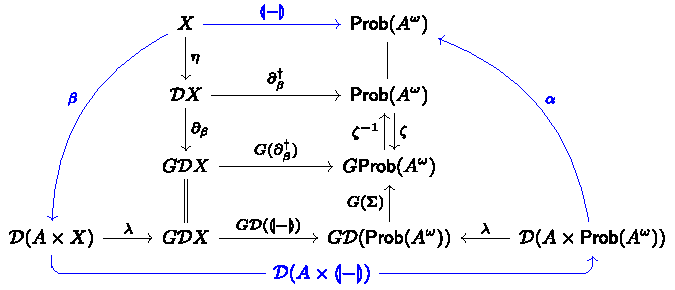
\includegraphics[width=324pt]{S5.Ex6.m1.g1.pdf}\end{center}
    The top square commutes by definition of %
% SOURCE HTML #S5.SS0.SSS0.Px2.SPx1.p3.m4
\hypertarget{html:S5.SS0.SSS0.Px2.SPx1.p3.m4}{}\({\llparenthesis{-}\rrparenthesis}\), the left part commutes as %
% SOURCE HTML #S5.SS0.SSS0.Px2.SPx1.p3.m5
\hypertarget{html:S5.SS0.SSS0.Px2.SPx1.p3.m5}{}\({\partial_{\beta}\circ\eta=\lambda\circ\beta}\) by definition of %
% SOURCE HTML #S5.SS0.SSS0.Px2.SPx1.p3.m6
\hypertarget{html:S5.SS0.SSS0.Px2.SPx1.p3.m6}{}\({\partial_{\beta}}\), the middle square commutes because %
% SOURCE HTML #S5.SS0.SSS0.Px2.SPx1.p3.m7
\hypertarget{html:S5.SS0.SSS0.Px2.SPx1.p3.m7}{}\({\partial_{\beta}^{\dagger}}\) is a coalgebra homomorphism, and the part on the bottom commutes by naturality of %
% SOURCE HTML #S5.SS0.SSS0.Px2.SPx1.p3.m8
\hypertarget{html:S5.SS0.SSS0.Px2.SPx1.p3.m8}{}\({\lambda}\). The commutativity of the remaining two parts is shown below.
\par\medskip
   %
% SOURCE HTML #S5.SS0.SSS0.Px2.SPx1.p4
\hypertarget{html:S5.SS0.SSS0.Px2.SPx1.p4}{} We first prove that %
% SOURCE HTML #S5.SS0.SSS0.Px2.SPx1.p4.m1
\hypertarget{html:S5.SS0.SSS0.Px2.SPx1.p4.m1}{}\({\zeta\circ\alpha=G(\Sigma)\circ\lambda}\), giving commutativity of the part on the right. For %
% SOURCE HTML #S5.SS0.SSS0.Px2.SPx1.p4.m2
\hypertarget{html:S5.SS0.SSS0.Px2.SPx1.p4.m2}{}\({\theta\in{\mathcal{D}}(A\times\text{\sf Prob}(A^{\omega}))}\), %
% SOURCE HTML #S5.SS0.SSS0.Px2.SPx1.p4.m3
\hypertarget{html:S5.SS0.SSS0.Px2.SPx1.p4.m3}{}\({a\in A}\), and %
% SOURCE HTML #S5.SS0.SSS0.Px2.SPx1.p4.m4
\hypertarget{html:S5.SS0.SSS0.Px2.SPx1.p4.m4}{}\({w\in A^{*}}\), we have, on the one hand:
\par\medskip
 %
% SOURCE HTML #S8.EGx8
\hypertarget{html:S8.EGx8}{} %
% SOURCE HTML #S5.Ex7
\hypertarget{html:S5.Ex7}{}  %
% SOURCE HTML #S5.Ex7.m1
\hypertarget{html:S5.Ex7.m1}{}\({\displaystyle\alpha(\theta)(B_{aw})}\) %
% SOURCE HTML #S5.Ex7.m2
\hypertarget{html:S5.Ex7.m2}{}\({\displaystyle=\sum_{\rho\in\text{\sf Prob}(A^{\omega})}\theta(a,\rho)\rho(B_{w})}\)   %
% SOURCE HTML #S5.E13
\hypertarget{html:S5.E13}{}  %
% SOURCE HTML #S5.E13.m1
\hypertarget{html:S5.E13.m1}{}\({\displaystyle\zeta(\alpha(\theta))(a)}\) %
% SOURCE HTML #S5.E13.m2
\hypertarget{html:S5.E13.m2}{}\({\displaystyle=\left\{\begin{array}[]{ll}\bot&\mbox{if $s_{a}=0$}\\
s_{a}\cdot(B_{w}\mapsto\sum_{\rho\in\text{\sf Prob}(A^{\omega})}\frac{\theta(a,\rho)}{s_{a}}\rho(B_{w}))&\mbox{if $s_{a}
eq 0$}\end{array}\right.}\)  (5.13)   We have used definitions of %
% SOURCE HTML #S5.SS0.SSS0.Px2.SPx1.p4.m5
\hypertarget{html:S5.SS0.SSS0.Px2.SPx1.p4.m5}{}\({\alpha}\) from (\hyperlink{html:S5.E10}{5.10}) and %
% SOURCE HTML #S5.SS0.SSS0.Px2.SPx1.p4.m6
\hypertarget{html:S5.SS0.SSS0.Px2.SPx1.p4.m6}{}\({\zeta}\) from (\hyperlink{html:S5.E6}{5.6}), that %
% SOURCE HTML #S5.SS0.SSS0.Px2.SPx1.p4.m7
\hypertarget{html:S5.SS0.SSS0.Px2.SPx1.p4.m7}{}\({aB_{w}=B_{aw}}\) and that %
% SOURCE HTML #S5.SS0.SSS0.Px2.SPx1.p4.m8
\hypertarget{html:S5.SS0.SSS0.Px2.SPx1.p4.m8}{}\({\alpha(\theta)(B_{a})=s_{a}}\). On the other hand, we use the definitions of %
% SOURCE HTML #S5.SS0.SSS0.Px2.SPx1.p4.m9
\hypertarget{html:S5.SS0.SSS0.Px2.SPx1.p4.m9}{}\({\lambda}\) from (\hyperlink{html:S5.E8}{5.8}) and %
% SOURCE HTML #S5.SS0.SSS0.Px2.SPx1.p4.m10
\hypertarget{html:S5.SS0.SSS0.Px2.SPx1.p4.m10}{}\({\Sigma}\) from (\hyperlink{html:S5.E5}{5.5}):
\par\medskip
 %
% SOURCE HTML #S8.EGx9
\hypertarget{html:S8.EGx9}{} %
% SOURCE HTML #S5.Ex8
\hypertarget{html:S5.Ex8}{}  %
% SOURCE HTML #S5.Ex8.m1
\hypertarget{html:S5.Ex8.m1}{}\({\displaystyle\lambda_{\text{\sf Prob}(A^{\omega})}(\theta)(a)}\) %
% SOURCE HTML #S5.Ex8.m2
\hypertarget{html:S5.Ex8.m2}{}\({\displaystyle=\begin{cases}\bot&\mbox{if $s_{a}=0$}\\
s_{a}\cdot(\rho\mapsto\frac{\theta(a,\rho)}{s_{a}})&\mbox{if $s_{a}
eq 0$}\end{cases}}\)   %
% SOURCE HTML #S5.E14
\hypertarget{html:S5.E14}{}  %
% SOURCE HTML #S5.E14.m1
\hypertarget{html:S5.E14.m1}{}\({\displaystyle G(\Sigma)(\lambda_{\text{\sf Prob}(A^{\omega})}(\theta))(a)}\) %
% SOURCE HTML #S5.E14.m2
\hypertarget{html:S5.E14.m2}{}\({\displaystyle=\begin{cases}\bot&\mbox{if $s_{a}=0$}\\
s_{a}\cdot(B_{w}\mapsto\sum_{\rho\in\text{\sf Prob}(A^{\omega})}\frac{\theta(a,\rho)}{s_{a}}\rho(B_{w}))&\mbox{if $s_{a}
eq 0$}\end{cases}}\)  (5.14)   Equations (\hyperlink{html:S5.Ex7}{5}) and (\hyperlink{html:S5.Ex8}{5}) now give %
% SOURCE HTML #S5.SS0.SSS0.Px2.SPx1.p4.m11
\hypertarget{html:S5.SS0.SSS0.Px2.SPx1.p4.m11}{}\({\zeta\circ\alpha=G(\Sigma)\circ\lambda}\).
\par\medskip
  %
% SOURCE HTML #S5.SS0.SSS0.Px2.SPx1.p5
\hypertarget{html:S5.SS0.SSS0.Px2.SPx1.p5}{} We turn to the commutativity of the remaining square. First, affineness of the map %
% SOURCE HTML #S5.SS0.SSS0.Px2.SPx1.p5.m1
\hypertarget{html:S5.SS0.SSS0.Px2.SPx1.p5.m1}{}\({\partial_{\beta}^{\dagger}:{\mathcal{D}}X\to\text{\sf Prob}(A^{\omega})}\) yields %
% SOURCE HTML #S5.SS0.SSS0.Px2.SPx1.p5.m2
\hypertarget{html:S5.SS0.SSS0.Px2.SPx1.p5.m2}{}\({\partial_{\beta}^{\dagger}\circ\mu_{X}=\Sigma\circ{\mathcal{D}}(\partial_{\beta}^{\dagger})}\). We precompose with %
% SOURCE HTML #S5.SS0.SSS0.Px2.SPx1.p5.m3
\hypertarget{html:S5.SS0.SSS0.Px2.SPx1.p5.m3}{}\({{\mathcal{D}}(\eta_{X})}\), and use the monad law %
% SOURCE HTML #S5.SS0.SSS0.Px2.SPx1.p5.m4
\hypertarget{html:S5.SS0.SSS0.Px2.SPx1.p5.m4}{}\({\mu_{X}\circ{\mathcal{D}}(\eta_{X})=\mathrm{id}_{{\mathcal{D}}X}}\) along with the definition of %
% SOURCE HTML #S5.SS0.SSS0.Px2.SPx1.p5.m5
\hypertarget{html:S5.SS0.SSS0.Px2.SPx1.p5.m5}{}\({\llparenthesis{-}\rrparenthesis}\). Thus %
% SOURCE HTML #S5.SS0.SSS0.Px2.SPx1.p5.m6
\hypertarget{html:S5.SS0.SSS0.Px2.SPx1.p5.m6}{}\({\partial_{\beta}^{\dagger}=\Sigma\circ{\mathcal{D}}(\llparenthesis{-}\rrparenthesis)}\). Now apply %
% SOURCE HTML #S5.SS0.SSS0.Px2.SPx1.p5.m7
\hypertarget{html:S5.SS0.SSS0.Px2.SPx1.p5.m7}{}\({G}\) to see the desired commutativity. %
% SOURCE HTML #S5.SS0.SSS0.Px2.SPx1.p5.m8
\hypertarget{html:S5.SS0.SSS0.Px2.SPx1.p5.m8}{}\({\hfill\blacktriangleleft}\)
\par\medskip
  %
% SOURCE HTML #S5.SS0.SSS0.Px2.SPx1.p6
\hypertarget{html:S5.SS0.SSS0.Px2.SPx1.p6}{} Returning to our blueprint for completeness in \hyperlink{html:S4}{Section 4}, \hyperlink{html:S5.Thmtheorem13}{Theorem 5.13} shows that %
% SOURCE HTML #S5.SS0.SSS0.Px2.SPx1.p6.m1
\hypertarget{html:S5.SS0.SSS0.Px2.SPx1.p6.m1}{}\({\left\llbracket{-}\right\rrbracket}\) arises from the final coalgebra map of %
% SOURCE HTML #S5.SS0.SSS0.Px2.SPx1.p6.m2
\hypertarget{html:S5.SS0.SSS0.Px2.SPx1.p6.m2}{}\({(\mathsf{PTerm},\tau)}\).
\par\medskip
    
%
% SOURCE HTML #S6
\hypertarget{html:S6}{} %
% SOURCE HTML #S6.m1
\hypertarget{html:S6.m1}{}%
% SOURCE HTML #S6.m2
\hypertarget{html:S6.m2}{}\section*{6 Step 2: \({\mathsf{PTerm}/{\equiv}}\) as a \({G}\)-coalgebra}
 %
% SOURCE HTML #S6.p1
\hypertarget{html:S6.p1}{} The set %
% SOURCE HTML #S6.p1.m1
\hypertarget{html:S6.p1.m1}{}\({\mathsf{PTerm}/{\equiv}}\) of provable equivalence classes of productive process terms inherits a canonical convex algebra structure from %
% SOURCE HTML #S6.p1.m2
\hypertarget{html:S6.p1.m2}{}\({\mathsf{PTerm}}\), given by %
% SOURCE HTML #S6.p1.m3
\hypertarget{html:S6.p1.m3}{}\({[e]\oplus_{r}[f]=[e\oplus_{r}f]}\). These operations are well-defined because \hyperlink{html:S3.F1}{Fig. 1} includes the necessary axiom and they are indeed convex operations as \hyperlink{html:S3.F1}{Fig. 1} includes the convex algebra axioms. In this section, we show that %
% SOURCE HTML #S6.p1.m4
\hypertarget{html:S6.p1.m4}{}\({\mathsf{PTerm}/{\equiv}}\) also carries a canonical %
% SOURCE HTML #S6.p1.m5
\hypertarget{html:S6.p1.m5}{}\({G}\)-coalgebra structure %
% SOURCE HTML #S6.p1.m6
\hypertarget{html:S6.p1.m6}{}\({(\mathsf{PTerm}/{\equiv},\partial)}\). We then focus on two goals: The first goal is to show that the stream semantics of a productive process term %
% SOURCE HTML #S6.p1.m7
\hypertarget{html:S6.p1.m7}{}\({e}\) is equal to the stream distribution %
% SOURCE HTML #S6.p1.m8
\hypertarget{html:S6.p1.m8}{}\({\partial^{\dagger}([e])}\) obtained from the finality of %
% SOURCE HTML #S6.p1.m9
\hypertarget{html:S6.p1.m9}{}\({(\text{\sf Prob}(A^{\omega}),\zeta)}\). The second goal of this section is to show that %
% SOURCE HTML #S6.p1.m10
\hypertarget{html:S6.p1.m10}{}\({(\mathsf{PTerm}/{\equiv},\partial)}\) is locally fg and that every ffg %
% SOURCE HTML #S6.p1.m11
\hypertarget{html:S6.p1.m11}{}\({G}\)-coalgebra admits a unique coalgebra homomorphism into %
% SOURCE HTML #S6.p1.m12
\hypertarget{html:S6.p1.m12}{}\({(\mathsf{PTerm}/{\equiv},\partial)}\).
\par\medskip
  %
% SOURCE HTML #S6.SS0.SSS0.P0.SPx1
\hypertarget{html:S6.SS0.SSS0.P0.SPx1}{} \par\noindent\textbf{Defining %
% SOURCE HTML #S6.SS0.SSS0.P0.SPx1.m1
\hypertarget{html:S6.SS0.SSS0.P0.SPx1.m1}{}\({\partial}\).}\quad  %
% SOURCE HTML #S6.SS0.SSS0.P0.SPx1.p1
\hypertarget{html:S6.SS0.SSS0.P0.SPx1.p1}{} Let %
% SOURCE HTML #S6.SS0.SSS0.P0.SPx1.p1.m1
\hypertarget{html:S6.SS0.SSS0.P0.SPx1.p1.m1}{}\({\tau(e)=\sum_{i=1}^{n}r_{i}\cdot(a_{i},e_{i})}\) and write %
% SOURCE HTML #S6.SS0.SSS0.P0.SPx1.p1.m2
\hypertarget{html:S6.SS0.SSS0.P0.SPx1.p1.m2}{}\({s_{a}=\sum_{a_{i}=a}r_{i}}\). We define the map %
% SOURCE HTML #S6.SS0.SSS0.P0.SPx1.p1.m3
\hypertarget{html:S6.SS0.SSS0.P0.SPx1.p1.m3}{}\({\partial\colon\mathsf{PTerm}/{\equiv}\to G(\mathsf{PTerm}/{\equiv})}\) using the formulas
\par\medskip
 %
% SOURCE HTML #S6.E1
\hypertarget{html:S6.E1}{}   %
% SOURCE HTML #S6.E1.m1
\hypertarget{html:S6.E1.m1}{}\[\mbox{\sf mass}_{\partial}(a,[e])=\sum_{a_{i}=a}r_{i}\qquad\mbox{\sf next}_{\partial}(a,[e])=\Big{[}\bigoplus_{i=1}^{n}(r_{i}/s_{a})\cdot e_{i}\Big{]}\]  (6.1)   for any %
% SOURCE HTML #S6.SS0.SSS0.P0.SPx1.p1.m4
\hypertarget{html:S6.SS0.SSS0.P0.SPx1.p1.m4}{}\({\equiv}\)-equivalence class %
% SOURCE HTML #S6.SS0.SSS0.P0.SPx1.p1.m5
\hypertarget{html:S6.SS0.SSS0.P0.SPx1.p1.m5}{}\({[e]\in\mathsf{PTerm}/{\equiv}}\) and %
% SOURCE HTML #S6.SS0.SSS0.P0.SPx1.p1.m6
\hypertarget{html:S6.SS0.SSS0.P0.SPx1.p1.m6}{}\({a\in A}\). It can be shown by induction on derivations that (\hyperlink{html:S6.E1}{6.1}) describes a well-defined map, i.e., %
% SOURCE HTML #S6.SS0.SSS0.P0.SPx1.p1.m7
\hypertarget{html:S6.SS0.SSS0.P0.SPx1.p1.m7}{}\({e\equiv f}\) implies the right-hand sides of the equations in (\hyperlink{html:S6.E1}{6.1}) agree.
\par\medskip
  %
% SOURCE HTML #S6.SS0.SSS0.P0.SPx1.p2
\hypertarget{html:S6.SS0.SSS0.P0.SPx1.p2}{} The following characterization of %
% SOURCE HTML #S6.SS0.SSS0.P0.SPx1.p2.m1
\hypertarget{html:S6.SS0.SSS0.P0.SPx1.p2.m1}{}\({(\mathsf{PTerm}/{\equiv},\partial)}\) illustrates that this is a natural choice of %
% SOURCE HTML #S6.SS0.SSS0.P0.SPx1.p2.m2
\hypertarget{html:S6.SS0.SSS0.P0.SPx1.p2.m2}{}\({G}\)-coalgebra structure on %
% SOURCE HTML #S6.SS0.SSS0.P0.SPx1.p2.m3
\hypertarget{html:S6.SS0.SSS0.P0.SPx1.p2.m3}{}\({\mathsf{PTerm}/{\equiv}}\).
\par\medskip
  %
% SOURCE HTML #S6.Thmtheorem1
\hypertarget{html:S6.Thmtheorem1}{} \par\noindent\textbf{\textbf{Lemma 6.1}\textbf{.}}\quad  %
% SOURCE HTML #S6.Thmtheorem1.p1
\hypertarget{html:S6.Thmtheorem1.p1}{} \emph{Given %
% SOURCE HTML #S6.Thmtheorem1.p1.m1
\hypertarget{html:S6.Thmtheorem1.p1.m1}{}\({e_{1},e_{2}\in\mathsf{PTerm}}\), let}
\par\medskip
 %
% SOURCE HTML #S6.Ex1
\hypertarget{html:S6.Ex1}{}   %
% SOURCE HTML #S6.Ex1.m1
\hypertarget{html:S6.Ex1.m1}{}\[\tau(e_{1})=\sum_{i=1}^{n}r_{i}\cdot(a_{i},f_{i})\qquad\tau(e_{2})=\sum_{i=1}^{n}s_{i}\cdot(a_{i},f_{i})\]    \emph{If %
% SOURCE HTML #S6.Thmtheorem1.p1.m2
\hypertarget{html:S6.Thmtheorem1.p1.m2}{}\({e_{1}\equiv e_{2}}\), then for any %
% SOURCE HTML #S6.Thmtheorem1.p1.m3
\hypertarget{html:S6.Thmtheorem1.p1.m3}{}\({a\in A}\),}
\par\medskip
 %
% SOURCE HTML #S6.E2
\hypertarget{html:S6.E2}{}   %
% SOURCE HTML #S6.E2.m1
\hypertarget{html:S6.E2.m1}{}\[r_{a}=s_{a}\qquad\text{ and }\qquad\bigoplus_{i=1}^{n}(r_{i}/r_{a})\cdot f_{i}\equiv\bigoplus_{i=1}^{n}(s_{i}/s_{a})\cdot f_{i}\]  (6.2)   \emph{where %
% SOURCE HTML #S6.Thmtheorem1.p1.m4
\hypertarget{html:S6.Thmtheorem1.p1.m4}{}\({r_{a}=\sum_{a_{i}=a}r_{i}}\) and %
% SOURCE HTML #S6.Thmtheorem1.p1.m5
\hypertarget{html:S6.Thmtheorem1.p1.m5}{}\({s_{a}=\sum_{a_{i}=a}s_{i}}\).}
\par\medskip
   %
% SOURCE HTML #S6.SS0.SSS0.P0.SPx1.p3
\hypertarget{html:S6.SS0.SSS0.P0.SPx1.p3}{} The proof of \hyperlink{html:S6.Thmtheorem1}{Lemma 6.1} is a rather long induction on the proof of %
% SOURCE HTML #S6.SS0.SSS0.P0.SPx1.p3.m1
\hypertarget{html:S6.SS0.SSS0.P0.SPx1.p3.m1}{}\({e\equiv f}\). As an immediate consequence of this lemma, we obtain the following.
\par\medskip
  %
% SOURCE HTML #S6.Thmtheorem2
\hypertarget{html:S6.Thmtheorem2}{} \par\noindent\textbf{\textbf{Lemma 6.2}\textbf{.}}\quad  %
% SOURCE HTML #S6.Thmtheorem2.p1
\hypertarget{html:S6.Thmtheorem2.p1}{} \emph{Let %
% SOURCE HTML #S6.Thmtheorem2.p1.m1
\hypertarget{html:S6.Thmtheorem2.p1.m1}{}\({({\mathcal{D}}(\mathsf{PTerm}),\partial_{\tau})=\Delta(\mathsf{PTerm},\tau)}\) and %
% SOURCE HTML #S6.Thmtheorem2.p1.m2
\hypertarget{html:S6.Thmtheorem2.p1.m2}{}\({h_{\Sigma}=([-])^{\#}}\) be the linear extension of the quotient-by-%
% SOURCE HTML #S6.Thmtheorem2.p1.m3
\hypertarget{html:S6.Thmtheorem2.p1.m3}{}\({\equiv}\) map. Then the following diagram commutes.}
\par\medskip
 %
% SOURCE HTML #S6.E3
\hypertarget{html:S6.E3}{}   %
% SOURCE HTML #S6.E3.m1.g1
\hypertarget{html:S6.E3.m1.g1}{}\begin{center}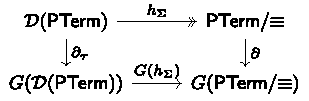
\includegraphics[width=148pt]{S6.E3.m1.g1.pdf}\end{center}
  (6.3)   \emph{In particular, %
% SOURCE HTML #S6.Thmtheorem2.p1.m4
\hypertarget{html:S6.Thmtheorem2.p1.m4}{}\({\partial}\) is a convex algebra homomorphism, and %
% SOURCE HTML #S6.Thmtheorem2.p1.m5
\hypertarget{html:S6.Thmtheorem2.p1.m5}{}\({(\mathsf{PTerm}/{\equiv},\partial)}\) is a homomorphic image of the determinized syntactic LMC.}
\par\medskip
   %
% SOURCE HTML #S6.Thmtheorem3
\hypertarget{html:S6.Thmtheorem3}{} \par\noindent\textbf{\textbf{Theorem 6.3}\textbf{.}}\quad  %
% SOURCE HTML #S6.Thmtheorem3.p1
\hypertarget{html:S6.Thmtheorem3.p1}{} \emph{For any %
% SOURCE HTML #S6.Thmtheorem3.p1.m1
\hypertarget{html:S6.Thmtheorem3.p1.m1}{}\({e\in\mathsf{PTerm}}\), %
% SOURCE HTML #S6.Thmtheorem3.p1.m2
\hypertarget{html:S6.Thmtheorem3.p1.m2}{}\({\left\llbracket{e}\right\rrbracket=\partial^{\dagger}([e])}\).}
\par\medskip
    %
% SOURCE HTML #S6.SS0.SSS0.P0.SPx2
\hypertarget{html:S6.SS0.SSS0.P0.SPx2}{} \par\noindent\textbf{Proof.}\quad  %
% SOURCE HTML #S6.SS0.SSS0.P0.SPx2.p1
\hypertarget{html:S6.SS0.SSS0.P0.SPx2.p1}{} By \hyperlink{html:S5.Thmtheorem9}{Theorem 5.9} and \hyperlink{html:S5.Thmtheorem13}{Theorem 5.13}, %
% SOURCE HTML #S6.SS0.SSS0.P0.SPx2.p1.m1
\hypertarget{html:S6.SS0.SSS0.P0.SPx2.p1.m1}{}\({\left\llbracket{e}\right\rrbracket=\partial_{\tau}^{\dagger}(1\cdot e)=\partial^{\dagger}\circ h_{\Sigma}(1\cdot e)=\partial^{\dagger}([e])}\). %
% SOURCE HTML #S6.SS0.SSS0.P0.SPx2.p1.m2
\hypertarget{html:S6.SS0.SSS0.P0.SPx2.p1.m2}{}\({\hfill\blacktriangleleft}\)
\par\medskip
  %
% SOURCE HTML #S6.Thmtheorem4
\hypertarget{html:S6.Thmtheorem4}{} \par\noindent\textbf{\textbf{Theorem 6.4}\textbf{.}}\quad  %
% SOURCE HTML #S6.Thmtheorem4.p1
\hypertarget{html:S6.Thmtheorem4.p1}{} \emph{The %
% SOURCE HTML #S6.Thmtheorem4.p1.m1
\hypertarget{html:S6.Thmtheorem4.p1.m1}{}\({G}\)-coalgebra %
% SOURCE HTML #S6.Thmtheorem4.p1.m2
\hypertarget{html:S6.Thmtheorem4.p1.m2}{}\({(\mathsf{PTerm}/{\equiv},\partial)}\) is locally fg.}
\par\medskip
    %
% SOURCE HTML #S6.SS0.SSS0.P0.SPx3
\hypertarget{html:S6.SS0.SSS0.P0.SPx3}{} \par\noindent\textbf{Proof.}\quad  %
% SOURCE HTML #S6.SS0.SSS0.P0.SPx3.p1
\hypertarget{html:S6.SS0.SSS0.P0.SPx3.p1}{} It follows from results due to Stark and Smolka [\hyperlink{html:bib.bib29}{29}] that the syntactic LMC %
% SOURCE HTML #S6.SS0.SSS0.P0.SPx3.p1.m1
\hypertarget{html:S6.SS0.SSS0.P0.SPx3.p1.m1}{}\({(\mathsf{PTerm},\tau)}\) is locally finite, in the sense that for any %
% SOURCE HTML #S6.SS0.SSS0.P0.SPx3.p1.m2
\hypertarget{html:S6.SS0.SSS0.P0.SPx3.p1.m2}{}\({e\in\mathsf{PTerm}}\), there is a finite subcoalgebra %
% SOURCE HTML #S6.SS0.SSS0.P0.SPx3.p1.m3
\hypertarget{html:S6.SS0.SSS0.P0.SPx3.p1.m3}{}\({(U,\tau_{U})}\) of %
% SOURCE HTML #S6.SS0.SSS0.P0.SPx3.p1.m4
\hypertarget{html:S6.SS0.SSS0.P0.SPx3.p1.m4}{}\({(\mathsf{PTerm},\tau)}\) containing %
% SOURCE HTML #S6.SS0.SSS0.P0.SPx3.p1.m5
\hypertarget{html:S6.SS0.SSS0.P0.SPx3.p1.m5}{}\({e}\). So, let %
% SOURCE HTML #S6.SS0.SSS0.P0.SPx3.p1.m6
\hypertarget{html:S6.SS0.SSS0.P0.SPx3.p1.m6}{}\({[e]\in\mathsf{PTerm}/{\equiv}}\) and find a finite subcoalgebra %
% SOURCE HTML #S6.SS0.SSS0.P0.SPx3.p1.m7
\hypertarget{html:S6.SS0.SSS0.P0.SPx3.p1.m7}{}\({(U,\tau_{U})}\) of %
% SOURCE HTML #S6.SS0.SSS0.P0.SPx3.p1.m8
\hypertarget{html:S6.SS0.SSS0.P0.SPx3.p1.m8}{}\({(\mathsf{PTerm},\tau)}\) containing %
% SOURCE HTML #S6.SS0.SSS0.P0.SPx3.p1.m9
\hypertarget{html:S6.SS0.SSS0.P0.SPx3.p1.m9}{}\({e}\). Then %
% SOURCE HTML #S6.SS0.SSS0.P0.SPx3.p1.m10
\hypertarget{html:S6.SS0.SSS0.P0.SPx3.p1.m10}{}\({\Delta(U,\tau_{U})}\) is a free fg subcoalgebra of %
% SOURCE HTML #S6.SS0.SSS0.P0.SPx3.p1.m11
\hypertarget{html:S6.SS0.SSS0.P0.SPx3.p1.m11}{}\({\Delta(\mathsf{PTerm},\tau)=({\mathcal{D}}(\mathsf{PTerm}),\partial_{\tau})}\) containing %
% SOURCE HTML #S6.SS0.SSS0.P0.SPx3.p1.m12
\hypertarget{html:S6.SS0.SSS0.P0.SPx3.p1.m12}{}\({1\cdot e}\). Taking the image of %
% SOURCE HTML #S6.SS0.SSS0.P0.SPx3.p1.m13
\hypertarget{html:S6.SS0.SSS0.P0.SPx3.p1.m13}{}\({\Delta(U,\tau_{U})}\) under %
% SOURCE HTML #S6.SS0.SSS0.P0.SPx3.p1.m14
\hypertarget{html:S6.SS0.SSS0.P0.SPx3.p1.m14}{}\({h_{\Sigma}}\), we obtain a finite subcoalgebra %
% SOURCE HTML #S6.SS0.SSS0.P0.SPx3.p1.m15
\hypertarget{html:S6.SS0.SSS0.P0.SPx3.p1.m15}{}\({(V,\partial_{V})=h_{\Sigma}(\Delta(U,\tau_{U}))}\) of %
% SOURCE HTML #S6.SS0.SSS0.P0.SPx3.p1.m16
\hypertarget{html:S6.SS0.SSS0.P0.SPx3.p1.m16}{}\({(\mathsf{PTerm}/{\equiv},\partial)}\) containing %
% SOURCE HTML #S6.SS0.SSS0.P0.SPx3.p1.m17
\hypertarget{html:S6.SS0.SSS0.P0.SPx3.p1.m17}{}\({[e]=h_{\Sigma}(1\cdot e)}\), as a quotient of a free fg %
% SOURCE HTML #S6.SS0.SSS0.P0.SPx3.p1.m18
\hypertarget{html:S6.SS0.SSS0.P0.SPx3.p1.m18}{}\({G}\)-coalgebra. Thus, %
% SOURCE HTML #S6.SS0.SSS0.P0.SPx3.p1.m19
\hypertarget{html:S6.SS0.SSS0.P0.SPx3.p1.m19}{}\({[e]}\) is contained in a fg subcoalgebra. %
% SOURCE HTML #S6.SS0.SSS0.P0.SPx3.p1.m20
\hypertarget{html:S6.SS0.SSS0.P0.SPx3.p1.m20}{}\({\hfill\blacktriangleleft}\)
\par\medskip
   %
% SOURCE HTML #S6.SSx1
\hypertarget{html:S6.SSx1}{} %
% SOURCE HTML #S6.SSx1.m1
\hypertarget{html:S6.SSx1.m1}{}\subsection*{Systems of equations from \({G}\)-coalgebras and their unique solutions}
 %
% SOURCE HTML #S6.SSx1.p1
\hypertarget{html:S6.SSx1.p1}{} The next goal is to show that every ffg %
% SOURCE HTML #S6.SSx1.p1.m1
\hypertarget{html:S6.SSx1.p1.m1}{}\({G}\)-coalgebra admits a unique coalgebra homomorphism into %
% SOURCE HTML #S6.SSx1.p1.m2
\hypertarget{html:S6.SSx1.p1.m2}{}\({(\mathsf{PTerm}/{\equiv},\partial)}\). As we remarked after \hyperlink{html:S5.Thmtheorem11}{Definition 5.11}, every ffg %
% SOURCE HTML #S6.SSx1.p1.m3
\hypertarget{html:S6.SSx1.p1.m3}{}\({G}\)-coalgebra is of the form %
% SOURCE HTML #S6.SSx1.p1.m4
\hypertarget{html:S6.SSx1.p1.m4}{}\({\Delta(X,\beta)}\) for some finite LMC %
% SOURCE HTML #S6.SSx1.p1.m5
\hypertarget{html:S6.SSx1.p1.m5}{}\({(X,\beta)}\). So, it suffices to show that every determinized finite LMC admits a unique coalgebra homomorphism into %
% SOURCE HTML #S6.SSx1.p1.m6
\hypertarget{html:S6.SSx1.p1.m6}{}\({\mathsf{PTerm}/{\equiv}}\). As we will see, each coalgebra homomorphism %
% SOURCE HTML #S6.SSx1.p1.m7
\hypertarget{html:S6.SSx1.p1.m7}{}\({\Delta(X,\beta)\to(\mathsf{PTerm}/{\equiv},\partial)}\) corresponds to a solution to a particular system of equations.
\par\medskip
  %
% SOURCE HTML #S6.Thmtheorem5
\hypertarget{html:S6.Thmtheorem5}{} \par\noindent\textbf{\textbf{Definition 6.5}\textbf{.}}\quad  %
% SOURCE HTML #S6.Thmtheorem5.p1
\hypertarget{html:S6.Thmtheorem5.p1}{} \emph{The \emph{guarded system of equations} corresponding to the finite LMC %
% SOURCE HTML #S6.Thmtheorem5.p1.m1
\hypertarget{html:S6.Thmtheorem5.p1.m1}{}\({(X,\beta)}\) is the set of formal equations}
\par\medskip
 %
% SOURCE HTML #S6.E4
\hypertarget{html:S6.E4}{}   %
% SOURCE HTML #S6.E4.m1
\hypertarget{html:S6.E4.m1}{}\[\mathcal{S}(X,\beta)=\Big{\{}x=\leavevmode\nobreak\ \bigoplus_{\mathclap{(a,y)\in A\times X}}\leavevmode\nobreak\ \beta(x)(a,y)\cdot ay\leavevmode\nobreak\ \Big{|}\leavevmode\nobreak\ x\in X\Big{\}}\]  (6.4)   \emph{A \emph{solution} to the guarded system of equations (\hyperlink{html:S6.E4}{6.4}) is a map}
\par\medskip
 %
% SOURCE HTML #S6.Ex2
\hypertarget{html:S6.Ex2}{}   %
% SOURCE HTML #S6.Ex2.m1
\hypertarget{html:S6.Ex2.m1}{}\[\varphi\colon X\to\mathsf{PTerm}\qquad\text{such that}\qquad(\forall x\in X)\leavevmode\nobreak\ \varphi(x)\equiv\leavevmode\nobreak\ \bigoplus_{\mathclap{(a,y)\in A\times X}}\leavevmode\nobreak\ \beta(x)(a,y)\cdot a\varphi(y)\]    \emph{Two solutions %
% SOURCE HTML #S6.Thmtheorem5.p1.m2
\hypertarget{html:S6.Thmtheorem5.p1.m2}{}\({\varphi,\psi}\) are \emph{equivalent}, written %
% SOURCE HTML #S6.Thmtheorem5.p1.m3
\hypertarget{html:S6.Thmtheorem5.p1.m3}{}\({\varphi\equiv\psi}\), if %
% SOURCE HTML #S6.Thmtheorem5.p1.m4
\hypertarget{html:S6.Thmtheorem5.p1.m4}{}\({\varphi(x)\equiv\psi(x)}\) for all %
% SOURCE HTML #S6.Thmtheorem5.p1.m5
\hypertarget{html:S6.Thmtheorem5.p1.m5}{}\({x\in X}\).}
\par\medskip
   %
% SOURCE HTML #S6.SSx1.p2
\hypertarget{html:S6.SSx1.p2}{} The following theorem was a key component of Stark and Smolka’s completeness proof for bisimilarity.
\par\medskip
  %
% SOURCE HTML #S6.Thmtheorem6
\hypertarget{html:S6.Thmtheorem6}{} \par\noindent\textbf{\textbf{Theorem 6.6}\textbf{ }(Stark-Smolka [\hyperlink{html:bib.bib29}{29}])\textbf{.}}\quad  %
% SOURCE HTML #S6.Thmtheorem6.p1
\hypertarget{html:S6.Thmtheorem6.p1}{} \emph{Every guarded finite system of equations has a unique solution up to %
% SOURCE HTML #S6.Thmtheorem6.p1.m1
\hypertarget{html:S6.Thmtheorem6.p1.m1}{}\({\equiv}\) without the use of the distributivity axiom %
% SOURCE HTML #S6.Thmtheorem6.p1.m2
\hypertarget{html:S6.Thmtheorem6.p1.m2}{}\({a(e\oplus_{r}f)=ae\oplus_{r}af}\).}
\par\medskip
   %
% SOURCE HTML #S6.SSx1.p3
\hypertarget{html:S6.SSx1.p3}{} An immediate consequence of the above theorem is the existence and uniqueness of solutions for systems of equations that arise from LMCs.
\par\medskip
  %
% SOURCE HTML #S6.Thmtheorem7
\hypertarget{html:S6.Thmtheorem7}{} \par\noindent\textbf{\textbf{Corollary 6.7}\textbf{.}}\quad  %
% SOURCE HTML #S6.Thmtheorem7.p1
\hypertarget{html:S6.Thmtheorem7.p1}{} \emph{Let %
% SOURCE HTML #S6.Thmtheorem7.p1.m1
\hypertarget{html:S6.Thmtheorem7.p1.m1}{}\({(X,\beta)}\) be a finite LMC. Then %
% SOURCE HTML #S6.Thmtheorem7.p1.m2
\hypertarget{html:S6.Thmtheorem7.p1.m2}{}\({\mathcal{S}(X,\beta)}\) has a unique solution up to %
% SOURCE HTML #S6.Thmtheorem7.p1.m3
\hypertarget{html:S6.Thmtheorem7.p1.m3}{}\({\equiv}\).}
\par\medskip
   %
% SOURCE HTML #S6.SSx1.p4
\hypertarget{html:S6.SSx1.p4}{} Using the distributivity axiom, we can transform each equation in (\hyperlink{html:S6.E4}{6.4}) into an equivalent system of equations of the form
\par\medskip
 %
% SOURCE HTML #S6.Ex3
\hypertarget{html:S6.Ex3}{}   %
% SOURCE HTML #S6.Ex3.m1
\hypertarget{html:S6.Ex3.m1}{}\[x=\bigoplus_{a\in A}\mbox{\sf mass}(a,x)\cdot a\leavevmode\nobreak\ \mbox{\sf
next}(a,x)\]    where mass and next are derived from %
% SOURCE HTML #S6.SSx1.p4.m3
\hypertarget{html:S6.SSx1.p4.m3}{}\({\partial_{\beta}}\). This tells us that a map %
% SOURCE HTML #S6.SSx1.p4.m4
\hypertarget{html:S6.SSx1.p4.m4}{}\({\varphi\colon X\to\mathsf{PTerm}}\) is a solution to %
% SOURCE HTML #S6.SSx1.p4.m5
\hypertarget{html:S6.SSx1.p4.m5}{}\({\mathcal{S}(X,\beta)}\) if and only if for all %
% SOURCE HTML #S6.SSx1.p4.m6
\hypertarget{html:S6.SSx1.p4.m6}{}\({x\in X}\),
\par\medskip
 %
% SOURCE HTML #S6.Ex4
\hypertarget{html:S6.Ex4}{}   %
% SOURCE HTML #S6.Ex4.m1
\hypertarget{html:S6.Ex4.m1}{}\[\varphi(x)\equiv\bigoplus_{a\in A}\mbox{\sf mass}(a,x)\cdot a\leavevmode\nobreak\ \varphi(\mbox{\sf next}(a,x))\]    Solving systems of equations of this form is equivalent to finding %
% SOURCE HTML #S6.SSx1.p4.m7
\hypertarget{html:S6.SSx1.p4.m7}{}\({G}\)-coalgebra homomorphisms into %
% SOURCE HTML #S6.SSx1.p4.m8
\hypertarget{html:S6.SSx1.p4.m8}{}\({(\mathsf{PTerm}/{\equiv},\partial)}\).
\par\medskip
  %
% SOURCE HTML #S6.Thmtheorem8
\hypertarget{html:S6.Thmtheorem8}{} \par\noindent\textbf{\textbf{Lemma 6.8}\textbf{.}}\quad  %
% SOURCE HTML #S6.Thmtheorem8.p1
\hypertarget{html:S6.Thmtheorem8.p1}{} \emph{Let %
% SOURCE HTML #S6.Thmtheorem8.p1.m1
\hypertarget{html:S6.Thmtheorem8.p1.m1}{}\({(X,\beta)}\) be a finite LMC, and let %
% SOURCE HTML #S6.Thmtheorem8.p1.m2
\hypertarget{html:S6.Thmtheorem8.p1.m2}{}\({\varphi\colon X\to\mathsf{PTerm}}\). Define %
% SOURCE HTML #S6.Thmtheorem8.p1.m3
\hypertarget{html:S6.Thmtheorem8.p1.m3}{}\({s_{\beta}\colon{\mathcal{D}}(X)\to\mathsf{PTerm}/{\equiv}}\) to be the linear extension of the composition %
% SOURCE HTML #S6.Thmtheorem8.p1.m4
\hypertarget{html:S6.Thmtheorem8.p1.m4}{}\({[-]\circ\varphi\colon X\to\mathsf{PTerm}/{\equiv}}\). Then %
% SOURCE HTML #S6.Thmtheorem8.p1.m5
\hypertarget{html:S6.Thmtheorem8.p1.m5}{}\({\varphi}\) is a solution to %
% SOURCE HTML #S6.Thmtheorem8.p1.m6
\hypertarget{html:S6.Thmtheorem8.p1.m6}{}\({\mathcal{S}(X,\beta)}\) if and only if %
% SOURCE HTML #S6.Thmtheorem8.p1.m7
\hypertarget{html:S6.Thmtheorem8.p1.m7}{}\({s\colon\Delta(X,\beta)\to(\mathsf{PTerm}/{\equiv},\partial)}\) is a coalgebra homomorphism.}
\par\medskip
   %
% SOURCE HTML #S6.SSx1.p5
\hypertarget{html:S6.SSx1.p5}{} We immediately obtain the following theorem.
\par\medskip
  %
% SOURCE HTML #S6.Thmtheorem9
\hypertarget{html:S6.Thmtheorem9}{} \par\noindent\textbf{\textbf{Theorem 6.9}\textbf{.}}\quad  %
% SOURCE HTML #S6.Thmtheorem9.p1
\hypertarget{html:S6.Thmtheorem9.p1}{} \emph{Let %
% SOURCE HTML #S6.Thmtheorem9.p1.m1
\hypertarget{html:S6.Thmtheorem9.p1.m1}{}\({(X,\beta)}\) be a finite LMC. There is a unique %
% SOURCE HTML #S6.Thmtheorem9.p1.m2
\hypertarget{html:S6.Thmtheorem9.p1.m2}{}\({G}\)-coalgebra homomorphism %
% SOURCE HTML #S6.Thmtheorem9.p1.m3
\hypertarget{html:S6.Thmtheorem9.p1.m3}{}\({s_{\beta}\colon\Delta(X,\beta)\to(\mathsf{PTerm}/{\equiv},\partial)}\).}
\par\medskip
   %
% SOURCE HTML #S6.SSx1.p6
\hypertarget{html:S6.SSx1.p6}{} Hence, recalling that every ffg coalgebra arises via determinisation (see \hyperlink{html:S5.Thmtheorem12}{Proposition 5.12}) yields that we have a unique homomorphism from any ffg coalgebra to %
% SOURCE HTML #S6.SSx1.p6.m1
\hypertarget{html:S6.SSx1.p6.m1}{}\({(\mathsf{PTerm}/{\equiv},\partial)}\).
\par\medskip
   
%
% SOURCE HTML #S7
\hypertarget{html:S7}{} %
% SOURCE HTML #S7.m1
\hypertarget{html:S7.m1}{}\section*{7 Step 3: Properness of \({G}\)}
 %
% SOURCE HTML #S7.p1
\hypertarget{html:S7.p1}{} In this section, we finish the outline of completeness that we stated in \hyperlink{html:S4}{Section 4} by establishing that %
% SOURCE HTML #S7.p1.m1
\hypertarget{html:S7.p1.m1}{}\({G}\) is finitary, preserves surjective affine maps, and is proper. By \hyperlink{html:S4.Thmtheorem4}{Theorems 4.4}, \hyperlink{html:S6.Thmtheorem4}{6.4}, and \hyperlink{html:S6.Thmtheorem9}{6.9}, this allows us to conclude that %
% SOURCE HTML #S7.p1.m2
\hypertarget{html:S7.p1.m2}{}\({(\mathsf{PTerm}/{\equiv},\partial)}\) is the final locally fg %
% SOURCE HTML #S7.p1.m3
\hypertarget{html:S7.p1.m3}{}\({G}\)-coalgebra.
\par\medskip
  %
% SOURCE HTML #S7.Thmtheorem1
\hypertarget{html:S7.Thmtheorem1}{} \par\noindent\textbf{\textbf{Lemma 7.1}\textbf{.}}\quad  %
% SOURCE HTML #S7.Thmtheorem1.p1
\hypertarget{html:S7.Thmtheorem1.p1}{} %
% SOURCE HTML #S7.Thmtheorem1.p1.m1
\hypertarget{html:S7.Thmtheorem1.p1.m1}{}\({G}\)\emph{ preserves pullbacks, and hence monomorphisms.}
\par\medskip
   %
% SOURCE HTML #S7.p2
\hypertarget{html:S7.p2}{} Let us mention that monomorphisms in %
% SOURCE HTML #S7.p2.m1
\hypertarget{html:S7.p2.m1}{}\({\mathsf{CA}}\) are exactly those affine maps which are injective as set functions. This follows from the fact that %
% SOURCE HTML #S7.p2.m2
\hypertarget{html:S7.p2.m2}{}\({U\colon\mathsf{CA}\to\mathsf{Set}}\) is a right adjoint and thus preserves all limits, in particular all pullbacks. Recall that in any category monos are characterized as special pullbacks as in the square below. In particular, let %
% SOURCE HTML #S7.p2.m3
\hypertarget{html:S7.p2.m3}{}\({f:X\to Y}\) be a monomorphism in %
% SOURCE HTML #S7.p2.m4
\hypertarget{html:S7.p2.m4}{}\({\mathsf{CA}}\). Then the square below is a pullback (and conversely) in %
% SOURCE HTML #S7.p2.m5
\hypertarget{html:S7.p2.m5}{}\({\mathsf{CA}}\).
\par\medskip
 %
% SOURCE HTML #S7.Ex1
\hypertarget{html:S7.Ex1}{}   %
% SOURCE HTML #S7.Ex1.m1.g1
\hypertarget{html:S7.Ex1.m1.g1}{}\begin{center}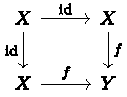
\includegraphics[width=61pt]{S7.Ex1.m1.g1.pdf}\end{center}
    Then its image under %
% SOURCE HTML #S7.p2.m6
\hypertarget{html:S7.p2.m6}{}\({U}\) is also a pullback and thus %
% SOURCE HTML #S7.p2.m7
\hypertarget{html:S7.p2.m7}{}\({U(f)}\) is a monomorphism in %
% SOURCE HTML #S7.p2.m8
\hypertarget{html:S7.p2.m8}{}\({\mathsf{Set}}\): that is, %
% SOURCE HTML #S7.p2.m9
\hypertarget{html:S7.p2.m9}{}\({f}\) is an injective function.
\par\medskip
  %
% SOURCE HTML #S7.p3
\hypertarget{html:S7.p3}{} For space reasons, we omit the proof that %
% SOURCE HTML #S7.p3.m1
\hypertarget{html:S7.p3.m1}{}\({G}\) preserves pullbacks. Using \hyperlink{html:S7.Thmtheorem1}{Lemma 7.1}, we can establish the first required property of %
% SOURCE HTML #S7.p3.m2
\hypertarget{html:S7.p3.m2}{}\({G}\).
\par\medskip
  %
% SOURCE HTML #S7.Thmtheorem2
\hypertarget{html:S7.Thmtheorem2}{} \par\noindent\textbf{\textbf{Lemma 7.2}\textbf{.}}\quad  %
% SOURCE HTML #S7.Thmtheorem2.p1
\hypertarget{html:S7.Thmtheorem2.p1}{} \emph{The functor %
% SOURCE HTML #S7.Thmtheorem2.p1.m1
\hypertarget{html:S7.Thmtheorem2.p1.m1}{}\({G:\mathsf{CA}\to\mathsf{CA}}\) on %
% SOURCE HTML #S7.Thmtheorem2.p1.m2
\hypertarget{html:S7.Thmtheorem2.p1.m2}{}\({\mathsf{CA}}\) is finitary.}
\par\medskip
   %
% SOURCE HTML #S7.SS0.SSS0.P0.SPx1
\hypertarget{html:S7.SS0.SSS0.P0.SPx1}{} \par\noindent\textbf{Proof.}\quad  %
% SOURCE HTML #S7.SS0.SSS0.P0.SPx1.p1
\hypertarget{html:S7.SS0.SSS0.P0.SPx1.p1}{} We are going to use the following results:
\par\medskip
 %
% SOURCE HTML #S7.I1
\hypertarget{html:S7.I1}{} %
% SOURCE HTML #S7.I1.ix1
\hypertarget{html:S7.I1.ix1}{}\textbf{Fact 1.}  %
% SOURCE HTML #S7.I1.ix1.p1
\hypertarget{html:S7.I1.ix1.p1}{} The forgetful functor %
% SOURCE HTML #S7.I1.ix1.p1.m1
\hypertarget{html:S7.I1.ix1.p1.m1}{}\({U\colon\mathsf{CA}\to\mathsf{Set}}\) creates directed colimits.
\par\medskip
   %
% SOURCE HTML #S7.I1.ix2
\hypertarget{html:S7.I1.ix2}{}\textbf{Fact 2.}  %
% SOURCE HTML #S7.I1.ix2.p1
\hypertarget{html:S7.I1.ix2.p1}{} Let %
% SOURCE HTML #S7.I1.ix2.p1.m1
\hypertarget{html:S7.I1.ix2.p1.m1}{}\({\mathsf{C}}\) be a category equipped with a functor %
% SOURCE HTML #S7.I1.ix2.p1.m2
\hypertarget{html:S7.I1.ix2.p1.m2}{}\({U\colon\mathsf{C}\to\mathsf{S}}\) that creates – hence, preserves and reflects – directed colimits. Let %
% SOURCE HTML #S7.I1.ix2.p1.m3
\hypertarget{html:S7.I1.ix2.p1.m3}{}\({G\colon\mathsf{C}\to\mathsf{C}}\) be a lifting of an endofunctor %
% SOURCE HTML #S7.I1.ix2.p1.m4
\hypertarget{html:S7.I1.ix2.p1.m4}{}\({H\colon\mathsf{S}\to\mathsf{S}}\), i.e., %
% SOURCE HTML #S7.I1.ix2.p1.m5
\hypertarget{html:S7.I1.ix2.p1.m5}{}\({U\circ G=H\circ U}\). Then, if %
% SOURCE HTML #S7.I1.ix2.p1.m6
\hypertarget{html:S7.I1.ix2.p1.m6}{}\({H}\) preserves directed colimits, so does %
% SOURCE HTML #S7.I1.ix2.p1.m7
\hypertarget{html:S7.I1.ix2.p1.m7}{}\({G}\).
\par\medskip
    In our situation, %
% SOURCE HTML #S7.SS0.SSS0.P0.SPx1.p1.m1
\hypertarget{html:S7.SS0.SSS0.P0.SPx1.p1.m1}{}\({G}\) is defined in \hyperlink{html:S5.E2}{Eq. 5.2}, %
% SOURCE HTML #S7.SS0.SSS0.P0.SPx1.p1.m2
\hypertarget{html:S7.SS0.SSS0.P0.SPx1.p1.m2}{}\({\mathsf{C}=\mathsf{CA}}\), and %
% SOURCE HTML #S7.SS0.SSS0.P0.SPx1.p1.m3
\hypertarget{html:S7.SS0.SSS0.P0.SPx1.p1.m3}{}\({\mathsf{S}=\mathsf{Set}}\). The proof of Fact 1 is routine, and similar to that of [\hyperlink{html:bib.bib1}{1}, Remark 3.4 (vii).(4)].
\par\medskip
  %
% SOURCE HTML #S7.SS0.SSS0.P0.SPx1.p2
\hypertarget{html:S7.SS0.SSS0.P0.SPx1.p2}{} Let us briefly establish Fact 2. Let %
% SOURCE HTML #S7.SS0.SSS0.P0.SPx1.p2.m1
\hypertarget{html:S7.SS0.SSS0.P0.SPx1.p2.m1}{}\({D\colon(I,\leq)\to\mathsf{C}}\) be a directed diagram in %
% SOURCE HTML #S7.SS0.SSS0.P0.SPx1.p2.m2
\hypertarget{html:S7.SS0.SSS0.P0.SPx1.p2.m2}{}\({\mathsf{C}}\), and let %
% SOURCE HTML #S7.SS0.SSS0.P0.SPx1.p2.m3
\hypertarget{html:S7.SS0.SSS0.P0.SPx1.p2.m3}{}\({(d_{i}\colon Di\to Y)_{i\in I}}\) be a colimiting cocone for %
% SOURCE HTML #S7.SS0.SSS0.P0.SPx1.p2.m4
\hypertarget{html:S7.SS0.SSS0.P0.SPx1.p2.m4}{}\({D}\). We want to show that %
% SOURCE HTML #S7.SS0.SSS0.P0.SPx1.p2.m5
\hypertarget{html:S7.SS0.SSS0.P0.SPx1.p2.m5}{}\({(G(d_{i})\colon GDi\to GY)_{i\in I}}\) is a colimiting cocone for %
% SOURCE HTML #S7.SS0.SSS0.P0.SPx1.p2.m6
\hypertarget{html:S7.SS0.SSS0.P0.SPx1.p2.m6}{}\({G\circ D}\). Since %
% SOURCE HTML #S7.SS0.SSS0.P0.SPx1.p2.m7
\hypertarget{html:S7.SS0.SSS0.P0.SPx1.p2.m7}{}\({U}\) reflects colimits, it suffices to show that %
% SOURCE HTML #S7.SS0.SSS0.P0.SPx1.p2.m8
\hypertarget{html:S7.SS0.SSS0.P0.SPx1.p2.m8}{}\({(UG(d_{i})\colon UGDi\to UGY)_{i\in I}}\) is a colimiting cocone for %
% SOURCE HTML #S7.SS0.SSS0.P0.SPx1.p2.m9
\hypertarget{html:S7.SS0.SSS0.P0.SPx1.p2.m9}{}\({U\circ G\circ D}\). To this end, consider the directed diagram %
% SOURCE HTML #S7.SS0.SSS0.P0.SPx1.p2.m10
\hypertarget{html:S7.SS0.SSS0.P0.SPx1.p2.m10}{}\({U\circ D\colon(I,\leq)\to\mathsf{S}}\). Since %
% SOURCE HTML #S7.SS0.SSS0.P0.SPx1.p2.m11
\hypertarget{html:S7.SS0.SSS0.P0.SPx1.p2.m11}{}\({U}\) preserves directed colimits, %
% SOURCE HTML #S7.SS0.SSS0.P0.SPx1.p2.m12
\hypertarget{html:S7.SS0.SSS0.P0.SPx1.p2.m12}{}\({(U(d_{i})\colon UDi\to UY)_{i\in I}}\) is a colimiting cocone for %
% SOURCE HTML #S7.SS0.SSS0.P0.SPx1.p2.m13
\hypertarget{html:S7.SS0.SSS0.P0.SPx1.p2.m13}{}\({U\circ D}\). Now, since %
% SOURCE HTML #S7.SS0.SSS0.P0.SPx1.p2.m14
\hypertarget{html:S7.SS0.SSS0.P0.SPx1.p2.m14}{}\({H}\) is finitary, i.e., it preserves directed colimits, %
% SOURCE HTML #S7.SS0.SSS0.P0.SPx1.p2.m15
\hypertarget{html:S7.SS0.SSS0.P0.SPx1.p2.m15}{}\({(HU(d_{i})\colon HUDi\to HUY)_{i\in I}}\) is a colimiting cocone of the directed diagram %
% SOURCE HTML #S7.SS0.SSS0.P0.SPx1.p2.m16
\hypertarget{html:S7.SS0.SSS0.P0.SPx1.p2.m16}{}\({H\circ U\circ D}\). But %
% SOURCE HTML #S7.SS0.SSS0.P0.SPx1.p2.m17
\hypertarget{html:S7.SS0.SSS0.P0.SPx1.p2.m17}{}\({H\circ U=U\circ G}\), so we can conclude that %
% SOURCE HTML #S7.SS0.SSS0.P0.SPx1.p2.m18
\hypertarget{html:S7.SS0.SSS0.P0.SPx1.p2.m18}{}\({(UG(d_{i})\colon UGDi\to UGY)_{i\in I}}\) is a colimiting cocone of the directed diagram %
% SOURCE HTML #S7.SS0.SSS0.P0.SPx1.p2.m19
\hypertarget{html:S7.SS0.SSS0.P0.SPx1.p2.m19}{}\({U\circ G\circ D}\), as desired.
\par\medskip
  %
% SOURCE HTML #S7.SS0.SSS0.P0.SPx1.p3
\hypertarget{html:S7.SS0.SSS0.P0.SPx1.p3}{} We can now proceed with the proof of the lemma. Recall from \hyperlink{html:S5.Thmtheorem6}{Remark 5.6} that %
% SOURCE HTML #S7.SS0.SSS0.P0.SPx1.p3.m1
\hypertarget{html:S7.SS0.SSS0.P0.SPx1.p3.m1}{}\({G}\) (from \hyperlink{html:S5.E2}{Eq. 5.2}) is a lifting of the endofunctor %
% SOURCE HTML #S7.SS0.SSS0.P0.SPx1.p3.m2
\hypertarget{html:S7.SS0.SSS0.P0.SPx1.p3.m2}{}\({H}\). The functor %
% SOURCE HTML #S7.SS0.SSS0.P0.SPx1.p3.m3
\hypertarget{html:S7.SS0.SSS0.P0.SPx1.p3.m3}{}\({H}\) is finitary because for any set %
% SOURCE HTML #S7.SS0.SSS0.P0.SPx1.p3.m4
\hypertarget{html:S7.SS0.SSS0.P0.SPx1.p3.m4}{}\({X}\), and any function %
% SOURCE HTML #S7.SS0.SSS0.P0.SPx1.p3.m5
\hypertarget{html:S7.SS0.SSS0.P0.SPx1.p3.m5}{}\({f\in HX}\), there is the finite set %
% SOURCE HTML #S7.SS0.SSS0.P0.SPx1.p3.m6
\hypertarget{html:S7.SS0.SSS0.P0.SPx1.p3.m6}{}\({Z=\{x\in X\mid\exists a\in A\exists r>0\text{ such that }f(a)=(r,x)\}}\) with %
% SOURCE HTML #S7.SS0.SSS0.P0.SPx1.p3.m7
\hypertarget{html:S7.SS0.SSS0.P0.SPx1.p3.m7}{}\({f\in HZ}\). By Fact 1, the forgetful functor %
% SOURCE HTML #S7.SS0.SSS0.P0.SPx1.p3.m8
\hypertarget{html:S7.SS0.SSS0.P0.SPx1.p3.m8}{}\({U\colon\mathsf{CA}\to\mathsf{Set}}\) creates directed colimits. Thus, the conditions of Fact 2 are satisfied, and we may conclude that %
% SOURCE HTML #S7.SS0.SSS0.P0.SPx1.p3.m9
\hypertarget{html:S7.SS0.SSS0.P0.SPx1.p3.m9}{}\({G}\) is finitary. %
% SOURCE HTML #S7.SS0.SSS0.P0.SPx1.p3.m10
\hypertarget{html:S7.SS0.SSS0.P0.SPx1.p3.m10}{}\({\hfill\blacktriangleleft}\)
\par\medskip
  %
% SOURCE HTML #S7.Thmtheorem3
\hypertarget{html:S7.Thmtheorem3}{} \par\noindent\textbf{\textbf{Lemma 7.3}\textbf{.}}\quad  %
% SOURCE HTML #S7.Thmtheorem3.p1
\hypertarget{html:S7.Thmtheorem3.p1}{} %
% SOURCE HTML #S7.Thmtheorem3.p1.m1
\hypertarget{html:S7.Thmtheorem3.p1.m1}{}\({G}\)\emph{ preserves surjective affine maps.}
\par\medskip
    %
% SOURCE HTML #S7.SS0.SSS0.P0.SPx2
\hypertarget{html:S7.SS0.SSS0.P0.SPx2}{} \par\noindent\textbf{Proof.}\quad  %
% SOURCE HTML #S7.SS0.SSS0.P0.SPx2.p1
\hypertarget{html:S7.SS0.SSS0.P0.SPx2.p1}{} Let %
% SOURCE HTML #S7.SS0.SSS0.P0.SPx2.p1.m1
\hypertarget{html:S7.SS0.SSS0.P0.SPx2.p1.m1}{}\({h\colon X\to Y}\) be a surjective affine map. Consider %
% SOURCE HTML #S7.SS0.SSS0.P0.SPx2.p1.m2
\hypertarget{html:S7.SS0.SSS0.P0.SPx2.p1.m2}{}\({G(h)\colon GX\to GY}\). For %
% SOURCE HTML #S7.SS0.SSS0.P0.SPx2.p1.m3
\hypertarget{html:S7.SS0.SSS0.P0.SPx2.p1.m3}{}\({a\in A}\), we have %
% SOURCE HTML #S7.SS0.SSS0.P0.SPx2.p1.m4
\hypertarget{html:S7.SS0.SSS0.P0.SPx2.p1.m4}{}\({G(h)(g)(a)(\bot)=\bot}\) and %
% SOURCE HTML #S7.SS0.SSS0.P0.SPx2.p1.m5
\hypertarget{html:S7.SS0.SSS0.P0.SPx2.p1.m5}{}\({G(h)(g)(a)(r\cdot x)=r\cdot h(x)}\).
\par\medskip
  %
% SOURCE HTML #S7.SS0.SSS0.P0.SPx2.p2
\hypertarget{html:S7.SS0.SSS0.P0.SPx2.p2}{} Take %
% SOURCE HTML #S7.SS0.SSS0.P0.SPx2.p2.m1
\hypertarget{html:S7.SS0.SSS0.P0.SPx2.p2.m1}{}\({f\in GY}\). For each %
% SOURCE HTML #S7.SS0.SSS0.P0.SPx2.p2.m2
\hypertarget{html:S7.SS0.SSS0.P0.SPx2.p2.m2}{}\({y\in Y}\), denote by %
% SOURCE HTML #S7.SS0.SSS0.P0.SPx2.p2.m3
\hypertarget{html:S7.SS0.SSS0.P0.SPx2.p2.m3}{}\({x_{y}}\) an element of %
% SOURCE HTML #S7.SS0.SSS0.P0.SPx2.p2.m4
\hypertarget{html:S7.SS0.SSS0.P0.SPx2.p2.m4}{}\({X}\) with %
% SOURCE HTML #S7.SS0.SSS0.P0.SPx2.p2.m5
\hypertarget{html:S7.SS0.SSS0.P0.SPx2.p2.m5}{}\({y=h(x_{y})}\). Such exists since %
% SOURCE HTML #S7.SS0.SSS0.P0.SPx2.p2.m6
\hypertarget{html:S7.SS0.SSS0.P0.SPx2.p2.m6}{}\({h}\) is surjective. We define %
% SOURCE HTML #S7.SS0.SSS0.P0.SPx2.p2.m7
\hypertarget{html:S7.SS0.SSS0.P0.SPx2.p2.m7}{}\({g\colon A\to X_{\bot}}\) as follows. For %
% SOURCE HTML #S7.SS0.SSS0.P0.SPx2.p2.m8
\hypertarget{html:S7.SS0.SSS0.P0.SPx2.p2.m8}{}\({a\in A}\), if %
% SOURCE HTML #S7.SS0.SSS0.P0.SPx2.p2.m9
\hypertarget{html:S7.SS0.SSS0.P0.SPx2.p2.m9}{}\({f(a)=\bot}\), set %
% SOURCE HTML #S7.SS0.SSS0.P0.SPx2.p2.m10
\hypertarget{html:S7.SS0.SSS0.P0.SPx2.p2.m10}{}\({g(a)=\bot}\) and if %
% SOURCE HTML #S7.SS0.SSS0.P0.SPx2.p2.m11
\hypertarget{html:S7.SS0.SSS0.P0.SPx2.p2.m11}{}\({f(a)=r\cdot y}\), set %
% SOURCE HTML #S7.SS0.SSS0.P0.SPx2.p2.m12
\hypertarget{html:S7.SS0.SSS0.P0.SPx2.p2.m12}{}\({g(a)=r\cdot x_{y}}\). Then %
% SOURCE HTML #S7.SS0.SSS0.P0.SPx2.p2.m13
\hypertarget{html:S7.SS0.SSS0.P0.SPx2.p2.m13}{}\({g\in GX}\) and %
% SOURCE HTML #S7.SS0.SSS0.P0.SPx2.p2.m14
\hypertarget{html:S7.SS0.SSS0.P0.SPx2.p2.m14}{}\({G(h)(g)=f}\). %
% SOURCE HTML #S7.SS0.SSS0.P0.SPx2.p2.m15
\hypertarget{html:S7.SS0.SSS0.P0.SPx2.p2.m15}{}\({\hfill\blacktriangleleft}\)
\par\medskip
  %
% SOURCE HTML #S7.SS0.SSS0.P0.SPx2.p3
\hypertarget{html:S7.SS0.SSS0.P0.SPx2.p3}{} The most interesting point in this section is the \emph{properness} of %
% SOURCE HTML #S7.SS0.SSS0.P0.SPx2.p3.m1
\hypertarget{html:S7.SS0.SSS0.P0.SPx2.p3.m1}{}\({G}\) (see \hyperlink{html:S7.Thmtheorem6}{Definition 7.6}). In order to verify that %
% SOURCE HTML #S7.SS0.SSS0.P0.SPx2.p3.m2
\hypertarget{html:S7.SS0.SSS0.P0.SPx2.p3.m2}{}\({G}\) is proper, we need a few lemmas regarding \emph{bisimilarity} and \emph{behavioural equivalence} for %
% SOURCE HTML #S7.SS0.SSS0.P0.SPx2.p3.m3
\hypertarget{html:S7.SS0.SSS0.P0.SPx2.p3.m3}{}\({G}\)-coalgebras.
\par\medskip
  %
% SOURCE HTML #S7.Thmtheorem4
\hypertarget{html:S7.Thmtheorem4}{} \par\noindent\textbf{\textbf{Lemma 7.4}\textbf{.}}\quad  %
% SOURCE HTML #S7.Thmtheorem4.p1
\hypertarget{html:S7.Thmtheorem4.p1}{} \emph{Let %
% SOURCE HTML #S7.Thmtheorem4.p1.m1
\hypertarget{html:S7.Thmtheorem4.p1.m1}{}\({(X,\gamma)}\) be a %
% SOURCE HTML #S7.Thmtheorem4.p1.m2
\hypertarget{html:S7.Thmtheorem4.p1.m2}{}\({G}\)-coalgebra on %
% SOURCE HTML #S7.Thmtheorem4.p1.m3
\hypertarget{html:S7.Thmtheorem4.p1.m3}{}\({\mathsf{CA}}\). Then bisimilarity (the largest bisimulation) on %
% SOURCE HTML #S7.Thmtheorem4.p1.m4
\hypertarget{html:S7.Thmtheorem4.p1.m4}{}\({(X,c)}\) coincides with behavioural equivalence, which in turn coincides with the final coalgebra semantics.}
\par\medskip
    %
% SOURCE HTML #S7.SS0.SSS0.P0.SPx3
\hypertarget{html:S7.SS0.SSS0.P0.SPx3}{} \par\noindent\textbf{Proof.}\quad  %
% SOURCE HTML #S7.SS0.SSS0.P0.SPx3.p1
\hypertarget{html:S7.SS0.SSS0.P0.SPx3.p1}{} Behavioural equivalence always coincides with the final coalgebra semantics if the functor admits a final coalgebra, which is the case for our functor %
% SOURCE HTML #S7.SS0.SSS0.P0.SPx3.p1.m1
\hypertarget{html:S7.SS0.SSS0.P0.SPx3.p1.m1}{}\({G}\) on %
% SOURCE HTML #S7.SS0.SSS0.P0.SPx3.p1.m2
\hypertarget{html:S7.SS0.SSS0.P0.SPx3.p1.m2}{}\({\mathsf{CA}}\).
\par\medskip
  %
% SOURCE HTML #S7.SS0.SSS0.P0.SPx3.p2
\hypertarget{html:S7.SS0.SSS0.P0.SPx3.p2}{} %
% SOURCE HTML #S7.SS0.SSS0.P0.SPx3.p2.m1
\hypertarget{html:S7.SS0.SSS0.P0.SPx3.p2.m1}{}\({\mathsf{CA}}\) is complete and cocomplete [\hyperlink{html:bib.bib2}{2}, § 9.3, Prop. 4] and the functor %
% SOURCE HTML #S7.SS0.SSS0.P0.SPx3.p2.m2
\hypertarget{html:S7.SS0.SSS0.P0.SPx3.p2.m2}{}\({G}\) preserves (weak) pullbacks by \hyperlink{html:S7.Thmtheorem1}{Lemma 7.1}. So %
% SOURCE HTML #S7.SS0.SSS0.P0.SPx3.p2.m3
\hypertarget{html:S7.SS0.SSS0.P0.SPx3.p2.m3}{}\({\mathsf{CA}}\) satisfies the requirements of [\hyperlink{html:bib.bib30}{30}, Theorem 4.1]. As a consequence: (1) every bisimulation is contained in a kernel bisimulation, and hence bisimilar states are behaviourally equivalent, and (2) every kernel bisimulation is a bisimulation, yielding that behaviourally equivalent states are bisimilar. %
% SOURCE HTML #S7.SS0.SSS0.P0.SPx3.p2.m4
\hypertarget{html:S7.SS0.SSS0.P0.SPx3.p2.m4}{}\({\hfill\blacktriangleleft}\)
\par\medskip
  %
% SOURCE HTML #S7.SS0.SSS0.P0.SPx3.p3
\hypertarget{html:S7.SS0.SSS0.P0.SPx3.p3}{} We need one more lemma that characterises bisimilarity for %
% SOURCE HTML #S7.SS0.SSS0.P0.SPx3.p3.m1
\hypertarget{html:S7.SS0.SSS0.P0.SPx3.p3.m1}{}\({G}\) in concrete terms. The proof follows directly from the definition of bisimulation.
\par\medskip
  %
% SOURCE HTML #S7.Thmtheorem5
\hypertarget{html:S7.Thmtheorem5}{} \par\noindent\textbf{\textbf{Lemma 7.5}\textbf{.}}\quad  %
% SOURCE HTML #S7.Thmtheorem5.p1
\hypertarget{html:S7.Thmtheorem5.p1}{} \emph{Let %
% SOURCE HTML #S7.Thmtheorem5.p1.m1
\hypertarget{html:S7.Thmtheorem5.p1.m1}{}\({(X,\gamma)}\) and %
% SOURCE HTML #S7.Thmtheorem5.p1.m2
\hypertarget{html:S7.Thmtheorem5.p1.m2}{}\({(Y,\vartheta)}\) be %
% SOURCE HTML #S7.Thmtheorem5.p1.m3
\hypertarget{html:S7.Thmtheorem5.p1.m3}{}\({G}\)-coalgebras. Let %
% SOURCE HTML #S7.Thmtheorem5.p1.m4
\hypertarget{html:S7.Thmtheorem5.p1.m4}{}\({R\subseteq X\times Y}\) be a subalgebra of %
% SOURCE HTML #S7.Thmtheorem5.p1.m5
\hypertarget{html:S7.Thmtheorem5.p1.m5}{}\({X\times Y}\). Then %
% SOURCE HTML #S7.Thmtheorem5.p1.m6
\hypertarget{html:S7.Thmtheorem5.p1.m6}{}\({R}\) is a bisimulation between %
% SOURCE HTML #S7.Thmtheorem5.p1.m7
\hypertarget{html:S7.Thmtheorem5.p1.m7}{}\({(X,\gamma)}\) and %
% SOURCE HTML #S7.Thmtheorem5.p1.m8
\hypertarget{html:S7.Thmtheorem5.p1.m8}{}\({(Y,\vartheta)}\) if and only if the following holds: whenever %
% SOURCE HTML #S7.Thmtheorem5.p1.m9
\hypertarget{html:S7.Thmtheorem5.p1.m9}{}\({a\in A}\) and %
% SOURCE HTML #S7.Thmtheorem5.p1.m10
\hypertarget{html:S7.Thmtheorem5.p1.m10}{}\({(x,y)\in R}\), %
% SOURCE HTML #S7.Thmtheorem5.p1.m11
\hypertarget{html:S7.Thmtheorem5.p1.m11}{}\({\mbox{\sf mass}_{\gamma}(a,x)=\mbox{\sf mass}_{\vartheta}(a,y)}\), and if %
% SOURCE HTML #S7.Thmtheorem5.p1.m12
\hypertarget{html:S7.Thmtheorem5.p1.m12}{}\({\mbox{\sf mass}_{\gamma}(a,x)=\mbox{\sf mass}_{\vartheta}(a,y)\neq 0}\), then %
% SOURCE HTML #S7.Thmtheorem5.p1.m13
\hypertarget{html:S7.Thmtheorem5.p1.m13}{}\({R}\) contains %
% SOURCE HTML #S7.Thmtheorem5.p1.m14
\hypertarget{html:S7.Thmtheorem5.p1.m14}{}\({(\mbox{\sf next}_{\gamma}(a,x),\mbox{\sf next}_{\vartheta}(a,y))}\).}
\par\medskip
   %
% SOURCE HTML #S7.SS0.SSS0.P0.SPx3.p4
\hypertarget{html:S7.SS0.SSS0.P0.SPx3.p4}{} Without further ado, let us now proceed with the proof that %
% SOURCE HTML #S7.SS0.SSS0.P0.SPx3.p4.m1
\hypertarget{html:S7.SS0.SSS0.P0.SPx3.p4.m1}{}\({G}\) is a proper functor, in the following sense.
\par\medskip
  %
% SOURCE HTML #S7.Thmtheorem6
\hypertarget{html:S7.Thmtheorem6}{} \par\noindent\textbf{\textbf{Definition 7.6}\textbf{.}}\quad  %
% SOURCE HTML #S7.Thmtheorem6.p1
\hypertarget{html:S7.Thmtheorem6.p1}{} \emph{Let %
% SOURCE HTML #S7.Thmtheorem6.p1.m1
\hypertarget{html:S7.Thmtheorem6.p1.m1}{}\({T}\) be a finitary monad on %
% SOURCE HTML #S7.Thmtheorem6.p1.m2
\hypertarget{html:S7.Thmtheorem6.p1.m2}{}\({\mathsf{Set}}\) and write %
% SOURCE HTML #S7.Thmtheorem6.p1.m3
\hypertarget{html:S7.Thmtheorem6.p1.m3}{}\({\mathsf{Set}^{T}}\) for the Eilenberg-Moore category of %
% SOURCE HTML #S7.Thmtheorem6.p1.m4
\hypertarget{html:S7.Thmtheorem6.p1.m4}{}\({T}\). A \emph{zig-zag} in %
% SOURCE HTML #S7.Thmtheorem6.p1.m5
\hypertarget{html:S7.Thmtheorem6.p1.m5}{}\({\mbox{\sf Coalg}_{\mathsf{Set}^{T}}(F)}\) is a diagram of the shape}
\par\medskip
 %
% SOURCE HTML #S7.E1
\hypertarget{html:S7.E1}{}\begin{center}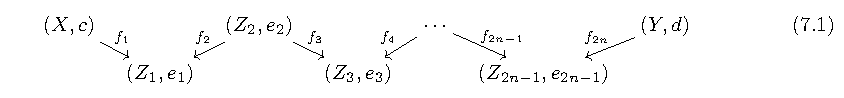
\includegraphics[width=.8\linewidth]{original-diagram-S7.E1-page18.pdf}\end{center}
 \emph{Write %
% SOURCE HTML #S7.Thmtheorem6.p1.m6
\hypertarget{html:S7.Thmtheorem6.p1.m6}{}\({\eta}\) for the unit of %
% SOURCE HTML #S7.Thmtheorem6.p1.m7
\hypertarget{html:S7.Thmtheorem6.p1.m7}{}\({T}\). The zig-zag above \emph{relates %
% SOURCE HTML #S7.Thmtheorem6.p1.m8
\hypertarget{html:S7.Thmtheorem6.p1.m8}{}\({x\in X}\) with %
% SOURCE HTML #S7.Thmtheorem6.p1.m9
\hypertarget{html:S7.Thmtheorem6.p1.m9}{}\({y\in Y}\)}, written %
% SOURCE HTML #S7.Thmtheorem6.p1.m10
\hypertarget{html:S7.Thmtheorem6.p1.m10}{}\({x\sim y}\), if there exist elements %
% SOURCE HTML #S7.Thmtheorem6.p1.m11
\hypertarget{html:S7.Thmtheorem6.p1.m11}{}\({z_{2k}\in Z_{2k}}\), %
% SOURCE HTML #S7.Thmtheorem6.p1.m12
\hypertarget{html:S7.Thmtheorem6.p1.m12}{}\({k=1,\ldots,n-1}\), with (setting %
% SOURCE HTML #S7.Thmtheorem6.p1.m13
\hypertarget{html:S7.Thmtheorem6.p1.m13}{}\({z_{0}=x}\) and %
% SOURCE HTML #S7.Thmtheorem6.p1.m14
\hypertarget{html:S7.Thmtheorem6.p1.m14}{}\({z_{2n}=y}\))}
\par\medskip
 %
% SOURCE HTML #S7.Ex2
\hypertarget{html:S7.Ex2}{}   %
% SOURCE HTML #S7.Ex2.m1
\hypertarget{html:S7.Ex2.m1}{}\[f_{2k}(z_{2k})=f_{2k-1}(z_{2k-2}),\quad k=1,\ldots,n\]    \emph{The endofunctor %
% SOURCE HTML #S7.Thmtheorem6.p1.m15
\hypertarget{html:S7.Thmtheorem6.p1.m15}{}\({F}\) is said to be \emph{proper} if the following statement holds: for any pair of ffg %
% SOURCE HTML #S7.Thmtheorem6.p1.m16
\hypertarget{html:S7.Thmtheorem6.p1.m16}{}\({F}\)-coalgebras %
% SOURCE HTML #S7.Thmtheorem6.p1.m17
\hypertarget{html:S7.Thmtheorem6.p1.m17}{}\({(T(X),c^{X})}\) and %
% SOURCE HTML #S7.Thmtheorem6.p1.m18
\hypertarget{html:S7.Thmtheorem6.p1.m18}{}\({(T(Y),c^{Y})}\) and any two elements %
% SOURCE HTML #S7.Thmtheorem6.p1.m19
\hypertarget{html:S7.Thmtheorem6.p1.m19}{}\({x\in X}\) and %
% SOURCE HTML #S7.Thmtheorem6.p1.m20
\hypertarget{html:S7.Thmtheorem6.p1.m20}{}\({y\in Y}\) with %
% SOURCE HTML #S7.Thmtheorem6.p1.m21
\hypertarget{html:S7.Thmtheorem6.p1.m21}{}\({\eta_{X}(x)\sim\eta_{Y}(y)}\), there exists a zig-zag in %
% SOURCE HTML #S7.Thmtheorem6.p1.m22
\hypertarget{html:S7.Thmtheorem6.p1.m22}{}\({\mbox{\sf Coalg}_{\mathsf{Set}^{T}}(F)}\) entirely consisting of ffg %
% SOURCE HTML #S7.Thmtheorem6.p1.m23
\hypertarget{html:S7.Thmtheorem6.p1.m23}{}\({F}\)-coalgebras that relates %
% SOURCE HTML #S7.Thmtheorem6.p1.m24
\hypertarget{html:S7.Thmtheorem6.p1.m24}{}\({\eta_{X}(x)}\) with %
% SOURCE HTML #S7.Thmtheorem6.p1.m25
\hypertarget{html:S7.Thmtheorem6.p1.m25}{}\({\eta_{Y}(y)}\). We may call such a zig-zag an ffg zig-zag.}
\par\medskip
   %
% SOURCE HTML #S7.Thmtheorem7
\hypertarget{html:S7.Thmtheorem7}{} \par\noindent\textbf{\textbf{Theorem 7.7}\textbf{.}}\quad  %
% SOURCE HTML #S7.Thmtheorem7.p1
\hypertarget{html:S7.Thmtheorem7.p1}{} \emph{The functor %
% SOURCE HTML #S7.Thmtheorem7.p1.m1
\hypertarget{html:S7.Thmtheorem7.p1.m1}{}\({G:\mathsf{CA}\to\mathsf{CA}}\) is proper.}
\par\medskip
    %
% SOURCE HTML #S7.SS0.SSS0.P0.SPx4
\hypertarget{html:S7.SS0.SSS0.P0.SPx4}{} \par\noindent\textbf{Proof.}\quad  %
% SOURCE HTML #S7.SS0.SSS0.P0.SPx4.p1
\hypertarget{html:S7.SS0.SSS0.P0.SPx4.p1}{} Consider two ffg %
% SOURCE HTML #S7.SS0.SSS0.P0.SPx4.p1.m1
\hypertarget{html:S7.SS0.SSS0.P0.SPx4.p1.m1}{}\({G}\)-coalgebras %
% SOURCE HTML #S7.SS0.SSS0.P0.SPx4.p1.m2
\hypertarget{html:S7.SS0.SSS0.P0.SPx4.p1.m2}{}\({({\mathcal{D}}(X),\partial_{\beta})}\) and %
% SOURCE HTML #S7.SS0.SSS0.P0.SPx4.p1.m3
\hypertarget{html:S7.SS0.SSS0.P0.SPx4.p1.m3}{}\({({\mathcal{D}}(Y),\partial_{\vartheta})}\), with behaviourally equivalent states %
% SOURCE HTML #S7.SS0.SSS0.P0.SPx4.p1.m4
\hypertarget{html:S7.SS0.SSS0.P0.SPx4.p1.m4}{}\({\varphi\in{\mathcal{D}}(X)}\) and %
% SOURCE HTML #S7.SS0.SSS0.P0.SPx4.p1.m5
\hypertarget{html:S7.SS0.SSS0.P0.SPx4.p1.m5}{}\({\psi\in{\mathcal{D}}(Y)}\). We need to relate %
% SOURCE HTML #S7.SS0.SSS0.P0.SPx4.p1.m6
\hypertarget{html:S7.SS0.SSS0.P0.SPx4.p1.m6}{}\({\varphi}\) and %
% SOURCE HTML #S7.SS0.SSS0.P0.SPx4.p1.m7
\hypertarget{html:S7.SS0.SSS0.P0.SPx4.p1.m7}{}\({\psi}\) with a suitable, ffg, zig-zag. We are going to use bisimilarity %
% SOURCE HTML #S7.SS0.SSS0.P0.SPx4.p1.m8
\hypertarget{html:S7.SS0.SSS0.P0.SPx4.p1.m8}{}\({B}\) on the coproduct coalgebra%
% SOURCE HTML #footnote2
\hypertarget{html:footnote2}{}\footnote{Left adjoints preserve colimits, so indeed the coproduct of free convex algebras is given by the formula %
% SOURCE HTML #footnote2.m1
\hypertarget{html:footnote2.m1}{}\({{\mathcal{D}}(X)+{\mathcal{D}}(Y)\cong{\mathcal{D}}(X+Y)}\), where the “%
% SOURCE HTML #footnote2.m2
\hypertarget{html:footnote2.m2}{}\({+}\)” on the left hand side is the coproduct in %
% SOURCE HTML #footnote2.m3
\hypertarget{html:footnote2.m3}{}\({\mathsf{CA}}\).} %
% SOURCE HTML #S7.SS0.SSS0.P0.SPx4.p1.m9
\hypertarget{html:S7.SS0.SSS0.P0.SPx4.p1.m9}{}\({({\mathcal{D}}(X),\partial_{\beta})+({\mathcal{D}}(Y),\partial_{\vartheta})\cong({\mathcal{D}}(X+Y),\partial_{\beta}+\partial_{\vartheta})}\).
\par\medskip
 %
% SOURCE HTML #S7.Ex3
\hypertarget{html:S7.Ex3}{}   %
% SOURCE HTML #S7.Ex3.m1.g1
\hypertarget{html:S7.Ex3.m1.g1}{}\begin{center}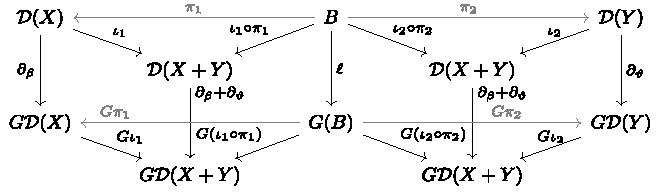
\includegraphics[width=317pt]{S7.Ex3.m1.g1.pdf}\end{center}
    where %
% SOURCE HTML #S7.SS0.SSS0.P0.SPx4.p1.m10
\hypertarget{html:S7.SS0.SSS0.P0.SPx4.p1.m10}{}\({\iota_{1},\iota_{2}}\) denote the coproduct injections. It remains to show that %
% SOURCE HTML #S7.SS0.SSS0.P0.SPx4.p1.m11
\hypertarget{html:S7.SS0.SSS0.P0.SPx4.p1.m11}{}\({B}\) is finitely generated as a subalgebra of the product %
% SOURCE HTML #S7.SS0.SSS0.P0.SPx4.p1.m12
\hypertarget{html:S7.SS0.SSS0.P0.SPx4.p1.m12}{}\({\mathsf{CA}}\), %
% SOURCE HTML #S7.SS0.SSS0.P0.SPx4.p1.m13
\hypertarget{html:S7.SS0.SSS0.P0.SPx4.p1.m13}{}\({{\mathcal{D}}(X+Y)\times{\mathcal{D}}(X+Y)}\). This follows from results below, using an analytic-algebraic characterization of finitely generated congruences (kernels of convex algebra homomorphisms) of finitely generated convex algebras.
\par\medskip
  %
% SOURCE HTML #S7.SS0.SSS0.P0.SPx4.p2
\hypertarget{html:S7.SS0.SSS0.P0.SPx4.p2}{} In more detail, note that we can identify any ffg algebra %
% SOURCE HTML #S7.SS0.SSS0.P0.SPx4.p2.m1
\hypertarget{html:S7.SS0.SSS0.P0.SPx4.p2.m1}{}\({{\mathcal{D}}(X)}\) with the simplex in the vector space %
% SOURCE HTML #S7.SS0.SSS0.P0.SPx4.p2.m2
\hypertarget{html:S7.SS0.SSS0.P0.SPx4.p2.m2}{}\({\mathbb{R}^{X}}\). This can be done by seeing each Dirac delta %
% SOURCE HTML #S7.SS0.SSS0.P0.SPx4.p2.m3
\hypertarget{html:S7.SS0.SSS0.P0.SPx4.p2.m3}{}\({1\cdot x}\) as a unit vector in %
% SOURCE HTML #S7.SS0.SSS0.P0.SPx4.p2.m4
\hypertarget{html:S7.SS0.SSS0.P0.SPx4.p2.m4}{}\({\mathbb{R}^{X}}\). Every congruence relation %
% SOURCE HTML #S7.SS0.SSS0.P0.SPx4.p2.m5
\hypertarget{html:S7.SS0.SSS0.P0.SPx4.p2.m5}{}\({R\subseteq{\mathcal{D}}(X)\times{\mathcal{D}}(X)}\) of convex algebras is a subalgebra of %
% SOURCE HTML #S7.SS0.SSS0.P0.SPx4.p2.m6
\hypertarget{html:S7.SS0.SSS0.P0.SPx4.p2.m6}{}\({{\mathcal{D}}(X)\times{\mathcal{D}}(X)}\), and so by extension can be identified with a (convex) subset of %
% SOURCE HTML #S7.SS0.SSS0.P0.SPx4.p2.m7
\hypertarget{html:S7.SS0.SSS0.P0.SPx4.p2.m7}{}\({\mathbb{R}^{X}\times\mathbb{R}^{X}\cong\mathbb{R}^{2X}}\). In particular, our %
% SOURCE HTML #S7.SS0.SSS0.P0.SPx4.p2.m8
\hypertarget{html:S7.SS0.SSS0.P0.SPx4.p2.m8}{}\({B}\) can be identified with a convex subset of %
% SOURCE HTML #S7.SS0.SSS0.P0.SPx4.p2.m9
\hypertarget{html:S7.SS0.SSS0.P0.SPx4.p2.m9}{}\({\mathbb{R}^{2(X+Y)}}\). As turns out, %
% SOURCE HTML #S7.SS0.SSS0.P0.SPx4.p2.m10
\hypertarget{html:S7.SS0.SSS0.P0.SPx4.p2.m10}{}\({B}\) is finitely generated as a subalgebra if and only if %
% SOURCE HTML #S7.SS0.SSS0.P0.SPx4.p2.m11
\hypertarget{html:S7.SS0.SSS0.P0.SPx4.p2.m11}{}\({B}\) is topologically closed in %
% SOURCE HTML #S7.SS0.SSS0.P0.SPx4.p2.m12
\hypertarget{html:S7.SS0.SSS0.P0.SPx4.p2.m12}{}\({\mathbb{R}^{2(X+Y)}}\). The following theorem is a direct consequence of Sokolova-Woracek [\hyperlink{html:bib.bib27}{27}, Proposition 5.9].
\par\medskip
  %
% SOURCE HTML #S7.Thmtheorem8
\hypertarget{html:S7.Thmtheorem8}{} \par\noindent\textbf{\textbf{Theorem 7.8}\textbf{.}}\quad  %
% SOURCE HTML #S7.Thmtheorem8.p1
\hypertarget{html:S7.Thmtheorem8.p1}{} \emph{Let %
% SOURCE HTML #S7.Thmtheorem8.p1.m1
\hypertarget{html:S7.Thmtheorem8.p1.m1}{}\({R\subseteq\mathbb{R}^{2X}}\) be a congruence on the ffg convex algebra %
% SOURCE HTML #S7.Thmtheorem8.p1.m2
\hypertarget{html:S7.Thmtheorem8.p1.m2}{}\({{\mathcal{D}}(X)\subseteq\mathbb{R}^{X}}\). Then %
% SOURCE HTML #S7.Thmtheorem8.p1.m3
\hypertarget{html:S7.Thmtheorem8.p1.m3}{}\({R}\) is finitely generated as a subalgebra if and only if it is topologically closed (closed under limits of Cauchy sequences).}
\par\medskip
   %
% SOURCE HTML #S7.Thmtheorem9
\hypertarget{html:S7.Thmtheorem9}{} \par\noindent\textbf{\textbf{Lemma 7.9}\textbf{.}}\quad  %
% SOURCE HTML #S7.Thmtheorem9.p1
\hypertarget{html:S7.Thmtheorem9.p1}{} \emph{Let %
% SOURCE HTML #S7.Thmtheorem9.p1.m1
\hypertarget{html:S7.Thmtheorem9.p1.m1}{}\({({\mathcal{D}}(X),\partial_{\beta})}\) be a %
% SOURCE HTML #S7.Thmtheorem9.p1.m2
\hypertarget{html:S7.Thmtheorem9.p1.m2}{}\({G}\)-coalgebra. Then for any %
% SOURCE HTML #S7.Thmtheorem9.p1.m3
\hypertarget{html:S7.Thmtheorem9.p1.m3}{}\({a\in A}\), the maps %
% SOURCE HTML #S7.Thmtheorem9.p1.m4
\hypertarget{html:S7.Thmtheorem9.p1.m4}{}\({\partial_{\beta}(-)(a)}\) and %
% SOURCE HTML #S7.Thmtheorem9.p1.m5
\hypertarget{html:S7.Thmtheorem9.p1.m5}{}\({\mbox{\sf mass}_{\beta}(a,-)}\) are restrictions of %
% SOURCE HTML #S7.Thmtheorem9.p1.m6
\hypertarget{html:S7.Thmtheorem9.p1.m6}{}\({\mathbb{R}}\)-linear maps %
% SOURCE HTML #S7.Thmtheorem9.p1.m7
\hypertarget{html:S7.Thmtheorem9.p1.m7}{}\({\mathbb{R}^{X}\to\mathbb{R}^{X+1}}\) and %
% SOURCE HTML #S7.Thmtheorem9.p1.m8
\hypertarget{html:S7.Thmtheorem9.p1.m8}{}\({\mathbb{R}^{X}\to\mathbb{R}}\) respectively.}
\par\medskip
    %
% SOURCE HTML #S7.SS0.SSS0.P0.SPx5
\hypertarget{html:S7.SS0.SSS0.P0.SPx5}{} \par\noindent\textbf{Proof.}\quad  %
% SOURCE HTML #S7.SS0.SSS0.P0.SPx5.p1
\hypertarget{html:S7.SS0.SSS0.P0.SPx5.p1}{} Recall that we think of the Dirac distributions %
% SOURCE HTML #S7.SS0.SSS0.P0.SPx5.p1.m1
\hypertarget{html:S7.SS0.SSS0.P0.SPx5.p1.m1}{}\({1\cdot x}\) as the basis vectors of %
% SOURCE HTML #S7.SS0.SSS0.P0.SPx5.p1.m2
\hypertarget{html:S7.SS0.SSS0.P0.SPx5.p1.m2}{}\({\mathbb{R}^{X}}\). We additionally have the unit vector %
% SOURCE HTML #S7.SS0.SSS0.P0.SPx5.p1.m3
\hypertarget{html:S7.SS0.SSS0.P0.SPx5.p1.m3}{}\({1\cdot\bot}\) in %
% SOURCE HTML #S7.SS0.SSS0.P0.SPx5.p1.m4
\hypertarget{html:S7.SS0.SSS0.P0.SPx5.p1.m4}{}\({\mathbb{R}^{X+1}}\). For %
% SOURCE HTML #S7.SS0.SSS0.P0.SPx5.p1.m5
\hypertarget{html:S7.SS0.SSS0.P0.SPx5.p1.m5}{}\({x\in X}\), write
\par\medskip
 %
% SOURCE HTML #S7.Ex4
\hypertarget{html:S7.Ex4}{}   %
% SOURCE HTML #S7.Ex4.m1
\hypertarget{html:S7.Ex4.m1}{}\[\partial_{\beta}(x)(a)=\sum_{y\in X}r_{xy}\cdot y\]    and %
% SOURCE HTML #S7.SS0.SSS0.P0.SPx5.p1.m6
\hypertarget{html:S7.SS0.SSS0.P0.SPx5.p1.m6}{}\({r_{x\bot}=1-\sum_{y\in X}r_{xy}}\). Define the matrix %
% SOURCE HTML #S7.SS0.SSS0.P0.SPx5.p1.m7
\hypertarget{html:S7.SS0.SSS0.P0.SPx5.p1.m7}{}\({M}\) by
\par\medskip
 %
% SOURCE HTML #S7.Ex5
\hypertarget{html:S7.Ex5}{}   %
% SOURCE HTML #S7.Ex5.m1
\hypertarget{html:S7.Ex5.m1}{}\[M=\begin{bmatrix}r_{x\xi}\leavevmode\nobreak\ \big{|}\leavevmode\nobreak\ x\in
X\text{ and }\xi\in X\cup\{\bot\}\end{bmatrix}\]    indexed by %
% SOURCE HTML #S7.SS0.SSS0.P0.SPx5.p1.m8
\hypertarget{html:S7.SS0.SSS0.P0.SPx5.p1.m8}{}\({X\times(X\cup\{\bot\})}\). A quick calculation verifies that indeed, for %
% SOURCE HTML #S7.SS0.SSS0.P0.SPx5.p1.m9
\hypertarget{html:S7.SS0.SSS0.P0.SPx5.p1.m9}{}\({\theta\in{\mathcal{D}}(X)}\), %
% SOURCE HTML #S7.SS0.SSS0.P0.SPx5.p1.m10
\hypertarget{html:S7.SS0.SSS0.P0.SPx5.p1.m10}{}\({\partial_{\beta}(\theta)(a)=M\theta}\) by linear extension. Of course, here we are thinking of %
% SOURCE HTML #S7.SS0.SSS0.P0.SPx5.p1.m11
\hypertarget{html:S7.SS0.SSS0.P0.SPx5.p1.m11}{}\({\theta=\sum_{x\in X}q_{x}\cdot x}\) as the column vector %
% SOURCE HTML #S7.SS0.SSS0.P0.SPx5.p1.m12
\hypertarget{html:S7.SS0.SSS0.P0.SPx5.p1.m12}{}\({[q_{x}\mid x\in X]}\).
\par\medskip
  %
% SOURCE HTML #S7.SS0.SSS0.P0.SPx5.p2
\hypertarget{html:S7.SS0.SSS0.P0.SPx5.p2}{} Similarly, define the row matrix %
% SOURCE HTML #S7.SS0.SSS0.P0.SPx5.p2.m1
\hypertarget{html:S7.SS0.SSS0.P0.SPx5.p2.m1}{}\({N=[1\mid x\in X]}\) of %
% SOURCE HTML #S7.SS0.SSS0.P0.SPx5.p2.m2
\hypertarget{html:S7.SS0.SSS0.P0.SPx5.p2.m2}{}\({1}\)’s. Then for %
% SOURCE HTML #S7.SS0.SSS0.P0.SPx5.p2.m3
\hypertarget{html:S7.SS0.SSS0.P0.SPx5.p2.m3}{}\({\theta=\sum_{x\in X}q_{x}\cdot x}\),
\par\medskip
 %
% SOURCE HTML #S7.Ex6
\hypertarget{html:S7.Ex6}{}   %
% SOURCE HTML #S7.Ex6.m1
\hypertarget{html:S7.Ex6.m1}{}\[N\theta=\begin{bmatrix}1&\cdots&1\end{bmatrix}[q_{x}\mid x\in X]=\sum_{x\in X}q_{x}\]    We therefore have %
% SOURCE HTML #S7.SS0.SSS0.P0.SPx5.p2.m4
\hypertarget{html:S7.SS0.SSS0.P0.SPx5.p2.m4}{}\({\mbox{\sf mass}_{\beta}(a,\theta)=NM\theta}\). Thus, both %
% SOURCE HTML #S7.SS0.SSS0.P0.SPx5.p2.m5
\hypertarget{html:S7.SS0.SSS0.P0.SPx5.p2.m5}{}\({\partial_{\beta}(-)(a)}\) and %
% SOURCE HTML #S7.SS0.SSS0.P0.SPx5.p2.m6
\hypertarget{html:S7.SS0.SSS0.P0.SPx5.p2.m6}{}\({\mbox{\sf mass}_{\beta}(a,-)}\) are restrictions of linear functions. %
% SOURCE HTML #S7.SS0.SSS0.P0.SPx5.p2.m7
\hypertarget{html:S7.SS0.SSS0.P0.SPx5.p2.m7}{}\({\hfill\blacktriangleleft}\)
\par\medskip
  %
% SOURCE HTML #S7.Thmtheorem10
\hypertarget{html:S7.Thmtheorem10}{} \par\noindent\textbf{\textbf{Corollary 7.10}\textbf{.}}\quad  %
% SOURCE HTML #S7.Thmtheorem10.p1
\hypertarget{html:S7.Thmtheorem10.p1}{} \emph{Let %
% SOURCE HTML #S7.Thmtheorem10.p1.m1
\hypertarget{html:S7.Thmtheorem10.p1.m1}{}\({({\mathcal{D}}(X),\partial_{\beta})}\) be a %
% SOURCE HTML #S7.Thmtheorem10.p1.m2
\hypertarget{html:S7.Thmtheorem10.p1.m2}{}\({G}\)-coalgebra. Then for any %
% SOURCE HTML #S7.Thmtheorem10.p1.m3
\hypertarget{html:S7.Thmtheorem10.p1.m3}{}\({a\in A}\), the maps %
% SOURCE HTML #S7.Thmtheorem10.p1.m4
\hypertarget{html:S7.Thmtheorem10.p1.m4}{}\({\partial_{\beta}(-)(a)}\) and %
% SOURCE HTML #S7.Thmtheorem10.p1.m5
\hypertarget{html:S7.Thmtheorem10.p1.m5}{}\({\mbox{\sf mass}_{\beta}(a,-)}\) are continuous.}
\par\medskip
    %
% SOURCE HTML #S7.SS0.SSS0.P0.SPx6
\hypertarget{html:S7.SS0.SSS0.P0.SPx6}{} \par\noindent\textbf{Proof.}\quad  %
% SOURCE HTML #S7.SS0.SSS0.P0.SPx6.p1
\hypertarget{html:S7.SS0.SSS0.P0.SPx6.p1}{} Follows directly from \hyperlink{html:S7.Thmtheorem9}{Lemma 7.9} and that %
% SOURCE HTML #S7.SS0.SSS0.P0.SPx6.p1.m1
\hypertarget{html:S7.SS0.SSS0.P0.SPx6.p1.m1}{}\({\mathbb{R}^{X}}\), %
% SOURCE HTML #S7.SS0.SSS0.P0.SPx6.p1.m2
\hypertarget{html:S7.SS0.SSS0.P0.SPx6.p1.m2}{}\({\mathbb{R}^{X+1}}\), and %
% SOURCE HTML #S7.SS0.SSS0.P0.SPx6.p1.m3
\hypertarget{html:S7.SS0.SSS0.P0.SPx6.p1.m3}{}\({\mathbb{R}}\) are finite dimensional. %
% SOURCE HTML #S7.SS0.SSS0.P0.SPx6.p1.m4
\hypertarget{html:S7.SS0.SSS0.P0.SPx6.p1.m4}{}\({\hfill\blacktriangleleft}\)
\par\medskip
  %
% SOURCE HTML #S7.Thmtheorem11
\hypertarget{html:S7.Thmtheorem11}{} \par\noindent\textbf{\textbf{Theorem 7.11}\textbf{.}}\quad  %
% SOURCE HTML #S7.Thmtheorem11.p1
\hypertarget{html:S7.Thmtheorem11.p1}{} \emph{Let %
% SOURCE HTML #S7.Thmtheorem11.p1.m1
\hypertarget{html:S7.Thmtheorem11.p1.m1}{}\({({\mathcal{D}}(X),\partial_{\beta})}\) and %
% SOURCE HTML #S7.Thmtheorem11.p1.m2
\hypertarget{html:S7.Thmtheorem11.p1.m2}{}\({({\mathcal{D}}(Y),\partial_{\vartheta})}\) be free finitely generated %
% SOURCE HTML #S7.Thmtheorem11.p1.m3
\hypertarget{html:S7.Thmtheorem11.p1.m3}{}\({G}\)-coalgebras. Let %
% SOURCE HTML #S7.Thmtheorem11.p1.m4
\hypertarget{html:S7.Thmtheorem11.p1.m4}{}\({(B,\ell)}\) be the largest bisimulation between %
% SOURCE HTML #S7.Thmtheorem11.p1.m5
\hypertarget{html:S7.Thmtheorem11.p1.m5}{}\({{\mathcal{D}}(X)}\) and %
% SOURCE HTML #S7.Thmtheorem11.p1.m6
\hypertarget{html:S7.Thmtheorem11.p1.m6}{}\({{\mathcal{D}}(Y)}\), and regard %
% SOURCE HTML #S7.Thmtheorem11.p1.m7
\hypertarget{html:S7.Thmtheorem11.p1.m7}{}\({B}\) as a subset of %
% SOURCE HTML #S7.Thmtheorem11.p1.m8
\hypertarget{html:S7.Thmtheorem11.p1.m8}{}\({{\mathcal{D}}(X+Y)\times{\mathcal{D}}(X+Y)\subseteq\mathbb{R}^{2(X+Y)}}\). Then %
% SOURCE HTML #S7.Thmtheorem11.p1.m9
\hypertarget{html:S7.Thmtheorem11.p1.m9}{}\({B}\) is a closed set and thus is finitely generated as a subalgebra.}
\par\medskip
    %
% SOURCE HTML #S7.SS0.SSS0.P0.SPx7
\hypertarget{html:S7.SS0.SSS0.P0.SPx7}{} \par\noindent\textbf{Proof.}\quad  %
% SOURCE HTML #S7.SS0.SSS0.P0.SPx7.p1
\hypertarget{html:S7.SS0.SSS0.P0.SPx7.p1}{} We show that the topological closure %
% SOURCE HTML #S7.SS0.SSS0.P0.SPx7.p1.m1
\hypertarget{html:S7.SS0.SSS0.P0.SPx7.p1.m1}{}\({\overline{B}}\) of %
% SOURCE HTML #S7.SS0.SSS0.P0.SPx7.p1.m2
\hypertarget{html:S7.SS0.SSS0.P0.SPx7.p1.m2}{}\({B\subseteq\mathbb{R}^{2(X+Y)}}\) is a bisimulation between %
% SOURCE HTML #S7.SS0.SSS0.P0.SPx7.p1.m3
\hypertarget{html:S7.SS0.SSS0.P0.SPx7.p1.m3}{}\({({\mathcal{D}}(X),\partial_{\beta})}\) and %
% SOURCE HTML #S7.SS0.SSS0.P0.SPx7.p1.m4
\hypertarget{html:S7.SS0.SSS0.P0.SPx7.p1.m4}{}\({({\mathcal{D}}(Y),\partial_{\vartheta})}\). Since %
% SOURCE HTML #S7.SS0.SSS0.P0.SPx7.p1.m5
\hypertarget{html:S7.SS0.SSS0.P0.SPx7.p1.m5}{}\({B}\) is the largest bisimulation, %
% SOURCE HTML #S7.SS0.SSS0.P0.SPx7.p1.m6
\hypertarget{html:S7.SS0.SSS0.P0.SPx7.p1.m6}{}\({B\subseteq\overline{B}\subseteq B}\).
\par\medskip
  %
% SOURCE HTML #S7.SS0.SSS0.P0.SPx7.p2
\hypertarget{html:S7.SS0.SSS0.P0.SPx7.p2}{} We appeal to \hyperlink{html:S7.Thmtheorem5}{Lemma 7.5}: Let %
% SOURCE HTML #S7.SS0.SSS0.P0.SPx7.p2.m1
\hypertarget{html:S7.SS0.SSS0.P0.SPx7.p2.m1}{}\({(\theta,\psi)\in\overline{B}}\). Then there is a Cauchy sequence %
% SOURCE HTML #S7.SS0.SSS0.P0.SPx7.p2.m2
\hypertarget{html:S7.SS0.SSS0.P0.SPx7.p2.m2}{}\({(\theta_{i},\psi_{i})_{i\in\mathbb{N}}}\) such that %
% SOURCE HTML #S7.SS0.SSS0.P0.SPx7.p2.m3
\hypertarget{html:S7.SS0.SSS0.P0.SPx7.p2.m3}{}\({(\theta_{i},\psi_{i})\to(\theta,\psi)}\) as %
% SOURCE HTML #S7.SS0.SSS0.P0.SPx7.p2.m4
\hypertarget{html:S7.SS0.SSS0.P0.SPx7.p2.m4}{}\({i\to\infty}\). This, in particular, means that %
% SOURCE HTML #S7.SS0.SSS0.P0.SPx7.p2.m5
\hypertarget{html:S7.SS0.SSS0.P0.SPx7.p2.m5}{}\({\theta_{i}\to\theta}\) and %
% SOURCE HTML #S7.SS0.SSS0.P0.SPx7.p2.m6
\hypertarget{html:S7.SS0.SSS0.P0.SPx7.p2.m6}{}\({\psi_{i}\to\psi}\) in the product topology. Now, for %
% SOURCE HTML #S7.SS0.SSS0.P0.SPx7.p2.m7
\hypertarget{html:S7.SS0.SSS0.P0.SPx7.p2.m7}{}\({a\in A}\),
\par\medskip
 %
% SOURCE HTML #S8.EGx10
\hypertarget{html:S8.EGx10}{} %
% SOURCE HTML #S7.Ex7
\hypertarget{html:S7.Ex7}{}  %
% SOURCE HTML #S7.Ex7.m1
\hypertarget{html:S7.Ex7.m1}{}\({\displaystyle\mbox{\sf mass}_{\beta}(a,\theta)}\) %
% SOURCE HTML #S7.Ex7.m2
\hypertarget{html:S7.Ex7.m2}{}\({\displaystyle=\mbox{\sf mass}_{\beta}(a,\lim\theta_{i})}\)   %
% SOURCE HTML #S7.Ex8
\hypertarget{html:S7.Ex8}{}   %
% SOURCE HTML #S7.Ex8.m1
\hypertarget{html:S7.Ex8.m1}{}\({\displaystyle=\lim\mbox{\sf mass}_{\beta}(a,\theta_{i})}\)  (\hyperlink{html:S7.Thmtheorem10}{Corollary 7.10})  %
% SOURCE HTML #S7.Ex9
\hypertarget{html:S7.Ex9}{}   %
% SOURCE HTML #S7.Ex9.m1
\hypertarget{html:S7.Ex9.m1}{}\({\displaystyle=\lim\mbox{\sf mass}_{\vartheta}(a,\psi_{i})}\)  (\hyperlink{html:S7.Thmtheorem5}{Lemma 7.5})  %
% SOURCE HTML #S7.Ex10
\hypertarget{html:S7.Ex10}{}   %
% SOURCE HTML #S7.Ex10.m1
\hypertarget{html:S7.Ex10.m1}{}\({\displaystyle=\mbox{\sf mass}_{\vartheta}(a,\lim\psi_{i})}\)  (\hyperlink{html:S7.Thmtheorem10}{Corollary 7.10})  %
% SOURCE HTML #S7.Ex11
\hypertarget{html:S7.Ex11}{}   %
% SOURCE HTML #S7.Ex11.m1
\hypertarget{html:S7.Ex11.m1}{}\({\displaystyle=\mbox{\sf mass}_{\vartheta}(a,\psi)}\)    This verifies the first condition. To verify the second, suppose that %
% SOURCE HTML #S7.SS0.SSS0.P0.SPx7.p2.m8
\hypertarget{html:S7.SS0.SSS0.P0.SPx7.p2.m8}{}\({\mbox{\sf mass}_{\beta}(a,\theta)=\mbox{\sf mass}_{\vartheta}(a,\psi)\neq 0}\). Then there is an %
% SOURCE HTML #S7.SS0.SSS0.P0.SPx7.p2.m9
\hypertarget{html:S7.SS0.SSS0.P0.SPx7.p2.m9}{}\({N>0}\) such that for all %
% SOURCE HTML #S7.SS0.SSS0.P0.SPx7.p2.m10
\hypertarget{html:S7.SS0.SSS0.P0.SPx7.p2.m10}{}\({i>N}\), %
% SOURCE HTML #S7.SS0.SSS0.P0.SPx7.p2.m11
\hypertarget{html:S7.SS0.SSS0.P0.SPx7.p2.m11}{}\({\mbox{\sf mass}_{\beta}(a,\theta_{i})=\mbox{\sf mass}_{\vartheta}(a,\psi_{i})>0}\). This allows for the following computation:
\par\medskip
 %
% SOURCE HTML #S7.Ex12
\hypertarget{html:S7.Ex12}{}   %
% SOURCE HTML #S7.Ex12.m1
\hypertarget{html:S7.Ex12.m1}{}\[\mbox{\sf next}_{\beta}(a,\theta)=\frac{\partial_{\beta}(\theta)(a)}{\mbox{\sf
mass}_{\beta}(a,\theta)}\overset{(*)}{=}\lim\frac{\partial_{\beta}(\theta_{i})(a)}{\mbox{\sf mass}_{\beta}(a,\theta_{i})}=\lim\mbox{\sf next}_{\beta}(a,\theta_{i})\]    and similarly for %
% SOURCE HTML #S7.SS0.SSS0.P0.SPx7.p2.m12
\hypertarget{html:S7.SS0.SSS0.P0.SPx7.p2.m12}{}\({\psi}\). Above, the step tagged (*) is due to the fact that a product of continuous functions is continuous on the intersection of their domain, which in this case contains all of the %
% SOURCE HTML #S7.SS0.SSS0.P0.SPx7.p2.m13
\hypertarget{html:S7.SS0.SSS0.P0.SPx7.p2.m13}{}\({\theta_{i}}\) as well as %
% SOURCE HTML #S7.SS0.SSS0.P0.SPx7.p2.m14
\hypertarget{html:S7.SS0.SSS0.P0.SPx7.p2.m14}{}\({\theta}\). Simply put, we use a known rule for computing limits of sequences of fractions: The limit of the pointwise-fractions of two sequences is the quotient of the two limits, given that the denominator sequence has non-zero limit. This tells us that
\par\medskip
 %
% SOURCE HTML #S7.Ex13
\hypertarget{html:S7.Ex13}{}   %
% SOURCE HTML #S7.Ex13.m1
\hypertarget{html:S7.Ex13.m1}{}\[(\mbox{\sf next}_{\beta}(a,\theta),\mbox{\sf next}_{\vartheta}(a,\psi))=\lim(\mbox{\sf next}_{\beta}(a,\theta_{i}),\mbox{\sf next}_{\vartheta}(a,\psi_{i}))\in\overline{B}\]    By \hyperlink{html:S7.Thmtheorem5}{Lemma 7.5}, %
% SOURCE HTML #S7.SS0.SSS0.P0.SPx7.p2.m15
\hypertarget{html:S7.SS0.SSS0.P0.SPx7.p2.m15}{}\({\overline{B}}\) is a bisimulation, as desired. %
% SOURCE HTML #S7.SS0.SSS0.P0.SPx7.p2.m16
\hypertarget{html:S7.SS0.SSS0.P0.SPx7.p2.m16}{}\({\hfill\blacktriangleleft}\)
\par\medskip
  %
% SOURCE HTML #S7.SS0.SSS0.P0.SPx7.p3
\hypertarget{html:S7.SS0.SSS0.P0.SPx7.p3}{} At long last, we complete the proof of \hyperlink{html:S7.Thmtheorem7}{Theorem 7.7} with an appeal to \hyperlink{html:S7.Thmtheorem11}{Theorem 7.11}. %
% SOURCE HTML #S7.SS0.SSS0.P0.SPx7.p3.m1
\hypertarget{html:S7.SS0.SSS0.P0.SPx7.p3.m1}{}\({\hfill\blacktriangleleft}\)
\par\medskip
   %
% SOURCE HTML #S7.SS0.SSS0.Px1
\hypertarget{html:S7.SS0.SSS0.Px1}{} \par\noindent\textbf{Recap of the proof of completeness, \hyperlink{html:S3.Thmtheorem6}{Theorem 3.6}}\quad  %
% SOURCE HTML #S7.SS0.SSS0.Px1.p1
\hypertarget{html:S7.SS0.SSS0.Px1.p1}{} We have taken the approach outlined in \hyperlink{html:S4}{Section 4} to showing that the axioms in \hyperlink{html:S3.F1}{Fig. 1} are complete with respect to the stream semantics of probabilistic process terms (\hyperlink{html:S2.Thmtheorem3}{Proposition 2.3}). In Step 1, we observed that the semantics map %
% SOURCE HTML #S7.SS0.SSS0.Px1.p1.m1
\hypertarget{html:S7.SS0.SSS0.Px1.p1.m1}{}\({\left\llbracket{-}\right\rrbracket}\) coincides with determinized stream semantics %
% SOURCE HTML #S7.SS0.SSS0.Px1.p1.m2
\hypertarget{html:S7.SS0.SSS0.Px1.p1.m2}{}\({\llparenthesis{-}\rrparenthesis}\) (\hyperlink{html:S5.Thmtheorem13}{Theorem 5.13}), and that in particular this meant that the final %
% SOURCE HTML #S7.SS0.SSS0.Px1.p1.m3
\hypertarget{html:S7.SS0.SSS0.Px1.p1.m3}{}\({G}\)-coalgebra homomorphism %
% SOURCE HTML #S7.SS0.SSS0.Px1.p1.m4
\hypertarget{html:S7.SS0.SSS0.Px1.p1.m4}{}\({\partial^{\dagger}\colon(\mathsf{PTerm}/{\equiv},\partial)\to(\text{\sf Prob}(A^{\omega}),\zeta)}\) satisfies %
% SOURCE HTML #S7.SS0.SSS0.Px1.p1.m5
\hypertarget{html:S7.SS0.SSS0.Px1.p1.m5}{}\({\left\llbracket{e}\right\rrbracket=\partial^{\dagger}([e])}\) for each %
% SOURCE HTML #S7.SS0.SSS0.Px1.p1.m6
\hypertarget{html:S7.SS0.SSS0.Px1.p1.m6}{}\({e\in\mathsf{PTerm}}\) (\hyperlink{html:S6.Thmtheorem3}{Theorem 6.3}). Thus, it suffices to show that %
% SOURCE HTML #S7.SS0.SSS0.Px1.p1.m7
\hypertarget{html:S7.SS0.SSS0.Px1.p1.m7}{}\({\partial^{\dagger}}\) is injective. To this end, we observed in \hyperlink{html:S4}{Section 4} that it suffices to construct a left inverse %
% SOURCE HTML #S7.SS0.SSS0.Px1.p1.m8
\hypertarget{html:S7.SS0.SSS0.Px1.p1.m8}{}\({k}\) to %
% SOURCE HTML #S7.SS0.SSS0.Px1.p1.m9
\hypertarget{html:S7.SS0.SSS0.Px1.p1.m9}{}\({q}\) in the diagram below.
\par\medskip
 %
% SOURCE HTML #S7.E2
\hypertarget{html:S7.E2}{}   %
% SOURCE HTML #S7.E2.m1.g1
\hypertarget{html:S7.E2.m1.g1}{}\begin{center}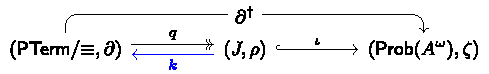
\includegraphics[width=235pt]{S7.E2.m1.g1.pdf}\end{center}
  (7.2)   The left inverse %
% SOURCE HTML #S7.SS0.SSS0.Px1.p1.m10
\hypertarget{html:S7.SS0.SSS0.Px1.p1.m10}{}\({k}\) in (\hyperlink{html:S7.E2}{7.2}) exists if %
% SOURCE HTML #S7.SS0.SSS0.Px1.p1.m11
\hypertarget{html:S7.SS0.SSS0.Px1.p1.m11}{}\({(\mathsf{PTerm}/{\equiv},\partial^{\dagger})}\) is the final locally fg %
% SOURCE HTML #S7.SS0.SSS0.Px1.p1.m12
\hypertarget{html:S7.SS0.SSS0.Px1.p1.m12}{}\({G}\)-coalgebra. In Step 2, we saw that %
% SOURCE HTML #S7.SS0.SSS0.Px1.p1.m13
\hypertarget{html:S7.SS0.SSS0.Px1.p1.m13}{}\({(\mathsf{PTerm}/{\equiv},\partial^{\dagger})}\) satisfies a slightly weaker universal property, that every ffg %
% SOURCE HTML #S7.SS0.SSS0.Px1.p1.m14
\hypertarget{html:S7.SS0.SSS0.Px1.p1.m14}{}\({G}\)-coalgebra admits a unique coalgebra homomorphism into it (\hyperlink{html:S6.Thmtheorem9}{Theorem 6.9}). In Step 3, we verified the hypotheses of \hyperlink{html:S4.Thmtheorem4}{Theorem 4.4}, in particular \hyperlink{html:S7.Thmtheorem7}{Theorem 7.7}, which tells us that in fact, %
% SOURCE HTML #S7.SS0.SSS0.Px1.p1.m15
\hypertarget{html:S7.SS0.SSS0.Px1.p1.m15}{}\({(\mathsf{PTerm}/{\equiv},\partial^{\dagger})}\) is the final locally fg coalgebra, as desired. This finishes the proof of completeness, \hyperlink{html:S3.Thmtheorem6}{Theorem 3.6}.
\par\medskip
   
%

% SOURCE HTML #S8
\hypertarget{html:S8}{} \section*{8 Discussion and Related Work}
 %
% SOURCE HTML #S8.p1
\hypertarget{html:S8.p1}{} We present the first sound and complete axiomatization of \emph{infinite} trace semantics for generative probabilistic transition systems, settling a recent conjecture of Schmid, Noquez, and Moss [\hyperlink{html:bib.bib21}{21}]. Our completeness theorem on infinite traces is a new direction in a series of coalgebraic completeness theorems on finite trace semantics for probabilistic process calculi [\hyperlink{html:bib.bib25}{25}, \hyperlink{html:bib.bib18}{18}], thus expanding the scope of this line of work. Our approach is categorical, and we build on recent results on proper functors over convex sets. In our proof, we use an analytic-algebraic result about convex congruences to show properness of %
% SOURCE HTML #S8.p1.m1
\hypertarget{html:S8.p1.m1}{}\({G}\). The particular functor which we prove to be proper has not been studied before, and the properness proof technique of [\hyperlink{html:bib.bib28}{28}] does not apply to it, but remarkably we could use a result concerning the geometry of convex congruences due to Sokolova and Woracek [\hyperlink{html:bib.bib27}{27}].
\par\medskip
  %
% SOURCE HTML #S8.p2
\hypertarget{html:S8.p2}{} We provide a characterization of infinite traces as the final coalgebra semantics of a functor over convex algebras. Infinite traces have been studied in the context of semantics of (variants of GPTS) before: via a largest homomorphism in the (order enriched) Kleisli category of the Giry monad [\hyperlink{html:bib.bib32}{32}] due to Urabe and Hasuo, via a greatest fixpoint in a category of generalised relations [\hyperlink{html:bib.bib4}{4}] due to Cîrstea, as a final coalgebra on a free positive convex algebra (a convex algebra with a distinguished element, i.e., in the Kleisli category of the subdistribution monad) due to Kerstan and König [\hyperlink{html:bib.bib9}{9}], and as a subcoalgebra of the final Moore automaton on a positive convex algebra (in the Eilenberg-Moore category of the subdistribution monad) due to Goy and Rot [\hyperlink{html:bib.bib5}{5}, \hyperlink{html:bib.bib6}{6}]. We offer a fourth characterization as a final coalgebra semantics for a new functor on convex algebras (i.e., in the Eilenberg-Moore category of the finite probability distribution monad) in \hyperlink{html:S5}{Section 5}. It is also the final coalgebra of a set functor.
\par\medskip
  %
% SOURCE HTML #S8.p3
\hypertarget{html:S8.p3}{} In the future, we want to explore whether the argument we provided for properness generalizes to other endofunctors on %
% SOURCE HTML #S8.p3.m1
\hypertarget{html:S8.p3.m1}{}\({\mathsf{CA}}\) and to endofunctors on the category of positive convex algebras used in [\hyperlink{html:bib.bib25}{25}, \hyperlink{html:bib.bib18}{18}]. We would like to expand our completeness theorem to incorporate hypotheses, especially in the context [\hyperlink{html:bib.bib21}{21}] where actions are interpreted concretely as contractions on a space: If the space and the contractions are fixed, the actions might satisfy additional relations. More speculatively, it might be interesting to also go in the opposite direction: Given a set of hypotheses, can one construct a canonical space and a contraction interpretation of the actions that satisfies the hypotheses? We would also like to consider different syntax for specifying LMCs and stream measures, such as the so-called formal language of recursion [\hyperlink{html:bib.bib7}{7}], which connects nicely to iterative algebra. Orthogonally, we would like to explore axiomatizations of behavioural distances, in the style of quantitative equational theories [\hyperlink{html:bib.bib12}{12}]. Last but not least, we would like to explore unifying the results of Silva and Sokolova [\hyperlink{html:bib.bib25}{25}] with those of this paper.
\par\medskip
  
%
% SOURCE HTML #bib
\hypertarget{html:bib}{} \par\noindent\textbf{References}\quad  
\begin{list}{}{\leftmargin=2em}
 %
% SOURCE HTML #bib.bib1
\hypertarget{html:bib.bib1}{}
\item[]  [1]  J. Adámek and J. Rosicky.  \emph{Locally Presentable and Accessible Categories}.  London Mathematical Society Lecture Note Series. Cambridge University Press, 1994.  
 %
% SOURCE HTML #bib.bib2
\hypertarget{html:bib.bib2}{}
\item[]  [2]  M. Barr and Ch. Wells.  \emph{Toposes, Triples and Theories}.  Springer, Berlin, 1985.  Revised and corrected version available from URL: \nolinkurl{www.cwru.edu/artsci/math/wells/pub/ttt.html.}  
 %
% SOURCE HTML #bib.bib3
\hypertarget{html:bib.bib3}{}
\item[]  [3]  F. Bartels, A. Sokolova, and E.P. de Vink.  A hierarchy of probabilistic system types.  \emph{Theoretical Computer Science}, 327:3–22, 2004.  \href{https://doi.org/10.1016/J.TCS.2004.07.019}{\nolinkurl{doi:10.1016/J.TCS.2004.07.019}}.  
 %
% SOURCE HTML #bib.bib4
\hypertarget{html:bib.bib4}{}
\item[]  [4]  Corina Cîrstea.  From branching to linear time, coalgebraically.  \emph{Fundam. Informaticae}, 150(3-4):379–406, 2017.  \href{https://doi.org/10.3233/FI-2017-1474}{\nolinkurl{doi:10.3233/FI-2017-1474}}.  
 %
% SOURCE HTML #bib.bib5
\hypertarget{html:bib.bib5}{}
\item[]  [5]  Alexandre Goy.  Trace semantics via determinization for probabilistic transition systems.  \emph{CoRR}, abs/1802.09084, 2018.  \href{https://arxiv.org/abs/1802.09084}{\texttt{arXiv:1802.09084}}.  
 %
% SOURCE HTML #bib.bib6
\hypertarget{html:bib.bib6}{}
\item[]  [6]  Alexandre Goy and Jurriaan Rot.  (In)finite trace equivalence of probabilistic transition systems.  In Corina Cîrstea, editor, \emph{Coalgebraic Methods in Computer Science - 14th IFIP WG 1.3 International Workshop, CMCS 2018}, volume 11202 of \emph{Lecture Notes in Computer Science}, pages 100–121. Springer, 2018.  \href{https://doi.org/10.1007/978-3-030-00389-0_7}{\nolinkurl{doi:10.1007/978-3-030-00389-0_7}}.  
 %
% SOURCE HTML #bib.bib7
\hypertarget{html:bib.bib7}{}
\item[]  [7]  Antonius J. C. Hurkens, Monica McArthur, Yiannis N. Moschovakis, Lawrence S. Moss, and Glen T. Whitney.  The logic of recursive equations.  \emph{J. Symb. Log.}, 63(2):451–478, 1998.  \href{https://doi.org/10.2307/2586843}{\nolinkurl{doi:10.2307/2586843}}.  
 %
% SOURCE HTML #bib.bib8
\hypertarget{html:bib.bib8}{}
\item[]  [8]  Bart Jacobs.  A bialgebraic review of deterministic automata, regular expressions and languages.  In Kokichi Futatsugi, Jean-Pierre Jouannaud, and José Meseguer, editors, \emph{Algebra, Meaning, and Computation, Essays Dedicated to Joseph A. Goguen on the Occasion of His 65th Birthday}, volume 4060 of \emph{Lecture Notes in Computer Science}, pages 375–404. Springer, 2006.  \href{https://doi.org/10.1007/11780274_20}{\nolinkurl{doi:10.1007/11780274_20}}.  
 %
% SOURCE HTML #bib.bib9
\hypertarget{html:bib.bib9}{}
\item[]  [9]  Henning Kerstan and Barbara König.  Coalgebraic Trace Semantics for Continuous Probabilistic Transition Systems.  \emph{Logical Methods in Computer Science}, Volume 9, Issue 4, December 2013.  \href{https://doi.org/10.2168/LMCS-9(4:16)2013}{\nolinkurl{doi:10.2168/LMCS-9(4:16)2013}}.  
 %
% SOURCE HTML #bib.bib10
\hypertarget{html:bib.bib10}{}
\item[]  [10]  S. C. Kleene.  Representation of events in nerve nets and finite automata.  In Claude Shannon and John McCarthy, editors, \emph{Automata Studies}, pages 3–41. Princeton University Press, Princeton, NJ, 1956.  
 %
% SOURCE HTML #bib.bib11
\hypertarget{html:bib.bib11}{}
\item[]  [11]  Kim Guldstrand Larsen and Arne Skou.  Bisimulation through probabilistic testing.  \emph{Inf. Comput.}, 94(1):1–28, 1991.  \href{https://doi.org/10.1016/0890-5401(91)90030-6}{\nolinkurl{doi:10.1016/0890-5401(91)90030-6}}.  
 %
% SOURCE HTML #bib.bib12
\hypertarget{html:bib.bib12}{}
\item[]  [12]  Radu Mardare, Prakash Panangaden, and Gordon Plotkin.  Quantitative algebraic reasoning.  In \emph{2016 31st Annual ACM/IEEE Symposium on Logic in Computer Science (LICS)}, pages 1–10, 2016.  
 %
% SOURCE HTML #bib.bib13
\hypertarget{html:bib.bib13}{}
\item[]  [13]  Stefan Milius.  A sound and complete calculus for finite stream circuits.  In \emph{Proceedings of the 25th Annual IEEE Symposium on Logic in Computer Science, LICS 2010}, pages 421–430. IEEE Computer Society, 2010.  \href{https://doi.org/10.1109/LICS.2010.11}{\nolinkurl{doi:10.1109/LICS.2010.11}}.  
 %
% SOURCE HTML #bib.bib14
\hypertarget{html:bib.bib14}{}
\item[]  [14]  Stefan Milius.  Proper functors and fixed points for finite behaviour.  \emph{Log. Methods Comput. Sci.}, 14(3), 2018.  \href{https://doi.org/10.23638/LMCS-14(3:22)2018}{\nolinkurl{doi:10.23638/LMCS-14(3:22)2018}}.  
 %
% SOURCE HTML #bib.bib15
\hypertarget{html:bib.bib15}{}
\item[]  [15]  Robin Milner.  A complete inference system for a class of regular behaviours.  \emph{J. Comput. Syst. Sci.}, 28(3):439–466, 1984.  \href{https://doi.org/10.1016/0022-0000(84)90023-0}{\nolinkurl{doi:10.1016/0022-0000(84)90023-0}}.  
 %
% SOURCE HTML #bib.bib16
\hypertarget{html:bib.bib16}{}
\item[]  [16]  Michael O. Rabin.  Probabilistic automata.  \emph{Inf. Control.}, 6(3):230–245, 1963.  \href{https://doi.org/10.1016/S0019-9958(63)90290-0}{\nolinkurl{doi:10.1016/S0019-9958(63)90290-0}}.  
 %
% SOURCE HTML #bib.bib17
\hypertarget{html:bib.bib17}{}
\item[]  [17]  Alexander Moshe Rabinovich.  A complete axiomatisation for trace congruence of finite state behaviors.  In Stephen D. Brookes, Michael G. Main, Austin Melton, Michael W. Mislove, and David A. Schmidt, editors, \emph{Mathematical Foundations of Programming Semantics, 9th International Conference, New Orleans, LA, USA, April 7-10, 1993, Proceedings}, volume 802 of \emph{Lecture Notes in Computer Science}, pages 530–543. Springer, 1993.  \href{https://doi.org/10.1007/3-540-58027-1_25}{\nolinkurl{doi:10.1007/3-540-58027-1_25}}.  
 %
% SOURCE HTML #bib.bib18
\hypertarget{html:bib.bib18}{}
\item[]  [18]  Wojciech Rozowski and Alexandra Silva.  A completeness theorem for probabilistic regular expressions.  In Pawel Sobocinski, Ugo Dal Lago, and Javier Esparza, editors, \emph{Proceedings of the 39th Annual ACM/IEEE Symposium on Logic in Computer Science, LICS 2024, Tallinn, Estonia, July 8-11, 2024}, pages 66:1–66:14. ACM, 2024.  \href{https://doi.org/10.1145/3661814.3662084}{\nolinkurl{doi:10.1145/3661814.3662084}}.  
 %
% SOURCE HTML #bib.bib19
\hypertarget{html:bib.bib19}{}
\item[]  [19]  Walter Rudin.  \emph{Real and Complex Analysis}.  McGraw-Hill, 1966.  
 %
% SOURCE HTML #bib.bib20
\hypertarget{html:bib.bib20}{}
\item[]  [20]  Jan J. M. M. Rutten.  Universal coalgebra: a theory of systems.  \emph{Theor. Comput. Sci.}, 249(1):3–80, 2000.  \href{https://doi.org/10.1016/S0304-3975(00)00056-6}{\nolinkurl{doi:10.1016/S0304-3975(00)00056-6}}.  
 %
% SOURCE HTML #bib.bib21
\hypertarget{html:bib.bib21}{}
\item[]  [21]  Todd Schmid, Victoria Noquez, and Lawrence S. Moss.  Fractals from regular behaviours.  In Paolo Baldan and Valeria de Paiva, editors, \emph{10th Conference on Algebra and Coalgebra in Computer Science, CALCO 2023, June 19-21, 2023, Indiana University Bloomington, IN, USA}, volume 270 of \emph{LIPIcs}, pages 14:1–14:18. Schloss Dagstuhl – Leibniz-Zentrum für Informatik, 2023.  Also available at https://arxiv.org/pdf/2306.03894.  \href{https://doi.org/10.4230/LIPICS.CALCO.2023.14}{\nolinkurl{doi:10.4230/LIPICS.CALCO.2023.14}}.  
 %
% SOURCE HTML #bib.bib22
\hypertarget{html:bib.bib22}{}
\item[]  [22]  Todd Schmid, Jurriaan Rot, and Alexandra Silva.  On star expressions and coalgebraic completeness theorems.  In Ana Sokolova, editor, \emph{Proceedings 37th Conference on Mathematical Foundations of Programming Semantics, MFPS 2021, Hybrid: Salzburg, Austria and Online, 30th August - 2nd September, 2021}, volume 351 of \emph{EPTCS}, pages 242–259, 2021.  \href{https://doi.org/10.4204/EPTCS.351.15}{\nolinkurl{doi:10.4204/EPTCS.351.15}}.  
 %
% SOURCE HTML #bib.bib23
\hypertarget{html:bib.bib23}{}
\item[]  [23]  Alexandra Silva, Filippo Bonchi, Marcello M. Bonsangue, and Jan J. M. M. Rutten.  Generalizing determinization from automata to coalgebras.  \emph{Log. Methods Comput. Sci.}, 9(1), 2013.  \href{https://doi.org/10.2168/LMCS-9(1:9)2013}{\nolinkurl{doi:10.2168/LMCS-9(1:9)2013}}.  
 %
% SOURCE HTML #bib.bib24
\hypertarget{html:bib.bib24}{}
\item[]  [24]  Alexandra Silva, Marcello M. Bonsangue, and Jan J. M. M. Rutten.  Non-deterministic kleene coalgebras.  \emph{Log. Methods Comput. Sci.}, 6(3), 2010.  URL: \href{http://arxiv.org/abs/1007.3769}{http://arxiv.org/abs/1007.3769}.  
 %
% SOURCE HTML #bib.bib25
\hypertarget{html:bib.bib25}{}
\item[]  [25]  Alexandra Silva and Ana Sokolova.  Sound and complete axiomatization of trace semantics for probabilistic systems.  In Michael W. Mislove and Joël Ouaknine, editors, \emph{Twenty-seventh Conference on the Mathematical Foundations of Programming Semantics, MFPS 2011, Pittsburgh, PA, USA, May 25-28, 2011}, volume 276 of \emph{Electronic Notes in Theoretical Computer Science}, pages 291–311. Elsevier, 2011.  \href{https://doi.org/10.1016/j.entcs.2011.09.027}{\nolinkurl{doi:10.1016/j.entcs.2011.09.027}}.  
 %
% SOURCE HTML #bib.bib26
\hypertarget{html:bib.bib26}{}
\item[]  [26]  A. Sokolova and E.P. de Vink.  Probabilistic automata: system types, parallel composition and comparison.  In C. Baier, B.R. Haverkort, H. Hermanns, J.-P. Katoen, and M. Siegle, editors, \emph{Validation of Stochastic Systems: A Guide to Current Research}, pages 1–43. LNCS 2925, 2004.  \href{https://doi.org/10.1007/978-3-540-24611-4_1}{\nolinkurl{doi:10.1007/978-3-540-24611-4_1}}.  
 %
% SOURCE HTML #bib.bib27
\hypertarget{html:bib.bib27}{}
\item[]  [27]  Ana Sokolova and Harald Woracek.  Congruences of convex algebras.  \emph{Journal of Pure and Applied Algebra}, 219(8):3110–3148, 2015.  \href{https://doi.org/10.1016/j.jpaa.2014.10.005}{\nolinkurl{doi:10.1016/j.jpaa.2014.10.005}}.  
 %
% SOURCE HTML #bib.bib28
\hypertarget{html:bib.bib28}{}
\item[]  [28]  Ana Sokolova and Harald Woracek.  Proper semirings and proper convex functors.  In \emph{FoSSaCS 2018}, pages 331–347. LNCS 10803, 2018.  
 %
% SOURCE HTML #bib.bib29
\hypertarget{html:bib.bib29}{}
\item[]  [29]  Eugene W. Stark and Scott A. Smolka.  A complete axiom system for finite-state probabilistic processes.  In Gordon D. Plotkin, Colin Stirling, and Mads Tofte, editors, \emph{Proof, Language, and Interaction, Essays in Honour of Robin Milner}, pages 571–596. The MIT Press, 2000.  
 %
% SOURCE HTML #bib.bib30
\hypertarget{html:bib.bib30}{}
\item[]  [30]  Sam Staton.  Relating coalgebraic notions of bisimulation.  In \emph{CALCO 2009}, volume 5728, pages 191–205. LNCS 5728, 2009.  \href{https://doi.org/10.1007/978-3-642-03741-2_14}{\nolinkurl{doi:10.1007/978-3-642-03741-2_14}}.  
 %
% SOURCE HTML #bib.bib31
\hypertarget{html:bib.bib31}{}
\item[]  [31]  T. Świrszcz.  Monadic functors and convexity.  \emph{Bull. Acad. Polon. Sci. Sér. Sci. Math. Astronom. Phys.}, 22:39–42, 1974.  
 %
% SOURCE HTML #bib.bib32
\hypertarget{html:bib.bib32}{}
\item[]  [32]  Natsuki Urabe and Ichiro Hasuo.  Coalgebraic infinite traces and Kleisli simulations.  \emph{Log. Methods Comput. Sci.}, 14(3), 2018.  \href{https://doi.org/10.23638/LMCS-14(3:15)2018}{\nolinkurl{doi:10.23638/LMCS-14(3:15)2018}}.  
 
\end{list}
 

\end{document}
